\documentclass[]{book}
\usepackage{lmodern}
\usepackage{setspace}
\setstretch{2}
\usepackage{amssymb,amsmath}
\usepackage{ifxetex,ifluatex}
\usepackage{fixltx2e} % provides \textsubscript
\ifnum 0\ifxetex 1\fi\ifluatex 1\fi=0 % if pdftex
  \usepackage[T1]{fontenc}
  \usepackage[utf8]{inputenc}
\else % if luatex or xelatex
  \ifxetex
    \usepackage{mathspec}
  \else
    \usepackage{fontspec}
  \fi
  \defaultfontfeatures{Ligatures=TeX,Scale=MatchLowercase}
    \setmainfont[]{FreeSerif}
\fi
% use upquote if available, for straight quotes in verbatim environments
\IfFileExists{upquote.sty}{\usepackage{upquote}}{}
% use microtype if available
\IfFileExists{microtype.sty}{%
\usepackage{microtype}
\UseMicrotypeSet[protrusion]{basicmath} % disable protrusion for tt fonts
}{}
\usepackage[margin=1in]{geometry}
\usepackage{hyperref}
\hypersetup{unicode=true,
            pdftitle={Knowledge of the U.S. Social Sciences},
            pdfauthor={Brooks Ambrose},
            pdfborder={0 0 0},
            breaklinks=true}
\urlstyle{same}  % don't use monospace font for urls
\usepackage{natbib}
\bibliographystyle{apalike}
\usepackage{longtable,booktabs}
\usepackage{graphicx,grffile}
\makeatletter
\def\maxwidth{\ifdim\Gin@nat@width>\linewidth\linewidth\else\Gin@nat@width\fi}
\def\maxheight{\ifdim\Gin@nat@height>\textheight\textheight\else\Gin@nat@height\fi}
\makeatother
% Scale images if necessary, so that they will not overflow the page
% margins by default, and it is still possible to overwrite the defaults
% using explicit options in \includegraphics[width, height, ...]{}
\setkeys{Gin}{width=\maxwidth,height=\maxheight,keepaspectratio}
\setlength{\emergencystretch}{3em}  % prevent overfull lines
\providecommand{\tightlist}{%
  \setlength{\itemsep}{0pt}\setlength{\parskip}{0pt}}
\setcounter{secnumdepth}{5}
% Redefines (sub)paragraphs to behave more like sections
\ifx\paragraph\undefined\else
\let\oldparagraph\paragraph
\renewcommand{\paragraph}[1]{\oldparagraph{#1}\mbox{}}
\fi
\ifx\subparagraph\undefined\else
\let\oldsubparagraph\subparagraph
\renewcommand{\subparagraph}[1]{\oldsubparagraph{#1}\mbox{}}
\fi

%%% Use protect on footnotes to avoid problems with footnotes in titles
\let\rmarkdownfootnote\footnote%
\def\footnote{\protect\rmarkdownfootnote}

%%% Change title format to be more compact
\usepackage{titling}

% Create subtitle command for use in maketitle
\newcommand{\subtitle}[1]{
  \posttitle{
    \begin{center}\large#1\end{center}
    }
}

\setlength{\droptitle}{-2em}

  \title{Knowledge of the U.S. Social Sciences}
    \pretitle{\vspace{\droptitle}\centering\huge}
  \posttitle{\par}
    \author{Brooks Ambrose}
    \preauthor{\centering\large\emph}
  \postauthor{\par}
      \predate{\centering\large\emph}
  \postdate{\par}
    \date{2019-09-02}

\usepackage{booktabs}
\usepackage{longtable}
\usepackage{array}
\usepackage{multirow}
\usepackage[table]{xcolor}
\usepackage{wrapfig}
\usepackage{float}
\usepackage{colortbl}
\usepackage{pdflscape}
\usepackage{tabu}
\usepackage{threeparttable}
\usepackage{threeparttablex}
\usepackage[normalem]{ulem}
\usepackage{makecell}
\usepackage{dcolumn}
\usepackage{longtable}
\usepackage{tabularx}
\floatplacement{figure}{H}
\usepackage[none]{hyphenat}
\raggedbottom
\usepackage{ragged2e}
\setlength{\RaggedRightParindent}{\parindent}
\RaggedRight

\usepackage{amsthm}
\newtheorem{theorem}{Theorem}[chapter]
\newtheorem{lemma}{Lemma}[chapter]
\theoremstyle{definition}
\newtheorem{definition}{Definition}[chapter]
\newtheorem{corollary}{Corollary}[chapter]
\newtheorem{proposition}{Proposition}[chapter]
\theoremstyle{definition}
\newtheorem{example}{Example}[chapter]
\theoremstyle{definition}
\newtheorem{exercise}{Exercise}[chapter]
\theoremstyle{remark}
\newtheorem*{remark}{Remark}
\newtheorem*{solution}{Solution}
\begin{document}
\maketitle

{
\setcounter{tocdepth}{2}
\tableofcontents
}
\listoftables
\listoffigures
\hypertarget{getting-started}{%
\chapter*{Getting Started}\label{getting-started}}


Dear reader,

Welcome! This study is available as a website,
\url{https://brooksambrose.github.io/portfolio}, and as a PDF document
downloadable from the website. Both are great ways to read the study.
The PDF makes for a quicker read, while the website offers additional
interactivity in figures and tables that will help you dive more deeply
into the exhibits.

\begin{figure}

{\centering 
\includegraphics[width=0.3\linewidth]{img/toolbar} 

}

\caption{Explore your options!}\label{fig:toolbar}
\end{figure}

At the top of the web page please notice a toolbar where you can:

\begin{itemize}
\tightlist
\item
  Show and hide the table of contents
\item
  Search the document
\item
  Adjust font and display settings
\item
  View the underlying code at GitHub.com
\item
  Download the PDF version
\end{itemize}

I hope you enjoy the study, and please feel free to report bugs,
comment, and collaborate at the issue tracker of the GitHub repository.

Best,\\
Brooks

\hypertarget{abstracts}{%
\section{Abstracts}\label{abstracts}}

\hypertarget{what-to-read-how-the-archive-pits-profession-against-education}{%
\subsection{What to Read? How the Archive pits Profession against
Education}\label{what-to-read-how-the-archive-pits-profession-against-education}}




























As scholarly fields of cultural production grow their
discourses tend to undergo a phase transition where hot global
tele-communication breaks down into cool parochial epicentrism. I
describe three structures--archives, profession, and education--whose
relationships explain the social and cultural forces leading to the
opening up and closing off of scholarly discourses. Given an archival
context, where expansive media collections give unlimited scope to
potential conversation topics, education tends to heat to a boil and
profession tends to cool to a condensation of discourses. When such
discursive tendencies (genres) are embedded in universities
(disciplines) the attendant competition over resources pits
professionals against educators and makes it possible to arrest cultural
dynamism into relatively static historical configurations. Such a social
domestication of cultural wildness allows knowledge to be harnessed for
economic purposes, namely workforce development (teaching) and product
design (research), and sometimes for political ends. These heteronomous
interests in predictable output from universities depresses their
cultural generativity. Such macroscopic historical tendencies are
difficult for the local agents of their development to recognize; their
myopic experience in university arenas is that of status conflicts
around investments in academic genres and fiscal conflicts around
investments in disciplinary personnel. Using the focal question scholars
new and old must answer--``What to read?''--I posit the genre-like
qualities of scholarly discourses and suggest the cognitive,
institutional, and social, that is disciplinary, consequences of
adhering to or abrogating genre conventions.




\textbf{Keywords}: profession, education, discipline, genre, labeling, status
exclusion

\hypertarget{social-science-disciplines-today}{%
\subsection{Social Science Disciplines
Today}\label{social-science-disciplines-today}}

















Social science is arranged into disciplines in a manner
similar to the genre systems of commercial fields of cultural production
(FCP) like music, yet evolving at a slower pace. Genres appear static
and given in the form of the labeling schemes of archivists and
librarians. Such schemes aim to describe academic genres objectively,
yet in so doing referencers and indexers reify them historically. Such
genre classifications are at times useful, frustrating, or didactic for
the academic ``disciples'' or knowledge workers of higher education.
This study maps the cognitive system of genre classifications in one
particular labeling scheme, that of the JSTOR historical archive, as
applied to one aspect of academic FCPs, journals. The patterns of
interdisciplinary cross labeling, of allowing journals to bear multiple
labels, are represented as a network and then visualized to reveal how
global axes among science, social science, and humanities condition the
local relationships of disciplines like sociology and anthropology.




\textbf{Keywords}: discipline, genre classification, network visualization,
community detection

\hypertarget{genre-and-the-literature}{%
\subsection{Genre and the Literature}\label{genre-and-the-literature}}





















In English the term \emph{genre} is a loanword from the
French term for \emph{kind}. As an analytical term in the social
sciences genre is a loanword from the humanities. The use of the term
varies greatly within and between disciplines. This study attempts a
metadisciplinary literature review of genre as a term found in a corpus
of JSTOR articles. I cast a very wide net by including any document in
English that includes the term genre in the title or abstract. The
resulting thousands of documents are ``read'' with the assistance of a
statistical topic model to classify documents into topics, that is,
strata of common vocabulary. I then perform content analysis on a
stratified sample of classified texts to compare their different uses of
the term genre. In an examination of the benefits and hazards of such a
distant reading approach, I outline a battery of diagnostics to examine
the validity of the topic model from both quantitative and qualitative
perspectives. Through a combination of machine distant reading and human
close reading, I arrive at a schema of five theories of the term genre.
In an argument for pandisciplinarity, I conclude with an analysis of the
logical possibility of new metaconcepts of genre that satisfy the
strictures of multiple disciplines.




\textbf{Keywords}: genre, disciplines, computational text analysis, topic
modeling, content analysis, digital humanities, distant reading

\hypertarget{vocabularies-of-anthropology-and-sociology-1888-1922}{%
\subsection{Vocabularies of Anthropology and Sociology,
1888-1922}\label{vocabularies-of-anthropology-and-sociology-1888-1922}}




Knowledge development of journals in sociology and
anthropology is measured as the change in topic prevalence over time.




\textbf{Keywords}: sociology of knowledge, topic modeling, history of social
science

\hypertarget{the-social-science-citation-landscape-1900-1940}{%
\subsection{The Social Science Citation Landscape,
1900-1940}\label{the-social-science-citation-landscape-1900-1940}}













Knowledge mapping of academic journals promotes the
conservation of intellectual history and stimulates discovery of
underexplored intellectual opportunities. Treated as a large network
community detection problem, I demonstrate how to apply the clique
percolation method to map two kinds of recorded knowledge: citations and
full text. The features of generated maps are explained, and
interpretive methods including visualization are presented. We use
American social science scholarship in the first third of the 20th
century prior to U.S. entry into World War II as a case, and describe
how the intellectual landscape of four separate social science
disciplines developed.




\textbf{Keywords}: citations, k-clique communities, community detection,
landscape

\hypertarget{int}{%
\chapter{What to Read? How the Archive pits Profession against
Education}\label{int}}

\hypertarget{abstract}{%
\subsubsection*{Abstract}\label{abstract}}


As scholarly fields of cultural production grow their
discourses tend to undergo a phase transition where hot global
tele-communication breaks down into cool parochial epicentrism. I
describe three structures--archives, profession, and education--whose
relationships explain the social and cultural forces leading to the
opening up and closing off of scholarly discourses. Given an archival
context, where expansive media collections give unlimited scope to
potential conversation topics, education tends to heat to a boil and
profession tends to cool to a condensation of discourses. When such
discursive tendencies (genres) are embedded in universities
(disciplines) the attendant competition over resources pits
professionals against educators and makes it possible to arrest cultural
dynamism into relatively static historical configurations. Such a social
domestication of cultural wildness allows knowledge to be harnessed for
economic purposes, namely workforce development (teaching) and product
design (research), and sometimes for political ends. These heteronomous
interests in predictable output from universities depresses their
cultural generativity. Such macroscopic historical tendencies are
difficult for the local agents of their development to recognize; their
myopic experience in university arenas is that of status conflicts
around investments in academic genres and fiscal conflicts around
investments in disciplinary personnel. Using the focal question scholars
new and old must answer--``What to read?''--I posit the genre-like
qualities of scholarly discourses and suggest the cognitive,
institutional, and social, that is disciplinary, consequences of
adhering to or abrogating genre conventions.

\hypertarget{keywords}{%
\subsubsection*{Keywords}\label{keywords}}


profession, education, discipline, genre, labeling, status
exclusion

\begin{center}\rule{0.5\linewidth}{\linethickness}\end{center}

The question of what to read is simple to be sure, but in fields of
scholarly consumption and production it is nonetheless fundamental.
Scholarship is a creative profession where a stock of cultural knowledge
forms a greater part of the infrastructure of production than in other
fields. This is not to say that other occupations, especially manual
ones, lack creativity. It is to say that in such fields knowledge has a
limited infrastructure. Whereas the know-how of the brick layer is black
boxed in her tools and technology and in the human capital she develops
by experience and tacit social learning, for the scholar as bricoleur
there exists in addition the distinctively overdeveloped feature of
cultural archiving as a universal memory. Except perhaps in outstanding
feats of primary research, contributions to scholarship are legitimate
to the extent that they have used the archive correctly. This problem of
using the archive, by which I mean all libraries and other organizations
that help scholars find published work, is easily expressed by the
question, ``what to read?'' Paradoxically, the over-development of the
archive induces a functional imperative: to the extent that more and
more of scholarship is memorable, mechanisms must develop to forget
large swaths of intellectual history. A person who studied a random draw
from the archive, even a monumental one, would no doubt qualify as an
educated person. Professionally, however, they would have answered the
question in a tragically wrong way. From the perspective of other
scholars, there are right and wrong choices about what to read. Because
it is so easy to access scholarly memory, the operative question really
becomes ``what not to read?''

Most occupations are not saddled with a heavy burden of memory,
remembering in the fashion of a Markov chain only the most recent
chapter in their history. Rather than in archives, memory is codified in
tools and technology. Though Internet search and self-publishing
services, especially video and image based ones, are creating
archive-like infrastructure for even manual occupations, the functions
are different. Contemporary Internet repositories provide knowledge as
factors of production to anyone who queries them, but many do not
purport to be archives in the sense that a historical record of cultural
products is preserved for posterity. They are much more concerned with
access to contemporaneous than to historical material, and indeed the
particular configuration of the contemporary that sells the most
advertisements ahead of search results. True historical archives of the
Internet, such as the Internet Archive or Common Crawl, are not used by
the public. Indeed why would they be; they expose the dizzying
complexity of the history of the Internet, which, even in only its
contemporaneous facet is already overwhelming. The Internet searcher
tends to be satisficing, and the search companies have refined their
ranking of results to meet their users' search budgets efficiently.

Searching and finding are different procedures; to search is to turn
over every rock, whereas to find is to turn over only the correct rock.
The searcher encounters many tricks before alighting on a treat, and
must make an effort to reject the false positives. The finder exploits
indexing technology that allows her to bypass the wrong material
altogether. Without a normative compulsion to make history accessible,
Internet search engines, which are actually find engines, avoid the
scholarly paradox of memory, which is that in the university system
great pains are made to remember everything just so that the correct
material may be forgotten. Scholars do not yet have find engines that
protect them from encountering irrelevant material, and it is a
professional competency to be able to quickly separate wheat from chaff.

\hypertarget{status-exclusion}{%
\section{Status exclusion}\label{status-exclusion}}

Though cultural abundance may be cultivated on the universal egalitarian
grounds that knowledge be made accessible to all, the complexity of the
archive creates an opportunity for the establishment of social
hierarchy. Because the archive's size so wildly outstrips individual and
organizational capacities to know its contents, methods of selection
become paramount. Indeed the power to control what counts as a
legitimate selection becomes a basis for authority and the conferral of
status. Status reflects a person's generalized ability or inability to
accrue resources to herself over the claims of others. Social
institutions define the conditions of status attainment, and different
institutions validate statuses according to different norms, truths, and
values. Knowledge as a valued resource mediates social relationships and
stabilizes status hierarchies differently in professions than in
education. The stability of status hierarchies depends on a qualified
segregation of these institutions, as the norms of one can be corrosive
to the norms of the other.

In the cynical view of professions, scholarship is the encryption of
memory by secret sets. If each field of professional scholarship is a
club, their passwords are particular lists of items from the archive.
Comers arriving with off list items or without enough of the correct
items may be held at the door, or if they are given entry, will be
marked with a scarlet letter. To say that the password items are the
only ones relevant to knowledge in the field is incredible; the depth of
the archive always impresses even the most experienced divers. The
importance of the list is not only in its knowledge potential but also
in its exclusionary function. Knowledge of the list is a qualification,
ignorance a disqualification for club membership.

Why check qualifications at all? The archive, in rendering knowledge
accessible and transparent, obviates a conventional function of
professions which is to restrict their ranks by controlling access to
secret knowledge. If the knowledge is not secret, a field must find
other mechanisms of exclusion to establish itself as a profession. To
make matters worse, the university contexts in which scholars work tend
to confront them with a public and to impose on them a duty of education
or service. Professionals who are embedded in markets trade the products
of their capacities, goods and services, for money. Their clients have
no serious interest in acquiring the professional's capacity to produce,
and this inscrutable cognitive base \citep[152]{DiMaggio1983Iron}
constitutes the client's experience of the professional's expertise.

Scholarship is based in the university and not in the market, and here
the value orientation to knowledge is very different. Professionals
default to entering into client, rather than peer, relationships. The
scholar's ``clients''--students, the public, and other scholars--may be
as interested in the production as they are in the product. From an
intellectual property perspective, ``ideas are strongly nonrival (they
are not used up) and only weakly excludable (they are difficult to
protect from use by others)'' \citep[278]{Thompson1995Conceptions}.
Because educational commitments promote the free flow of ideas,
knowledge qua knowledge cannot be the basis of professional exclusion
within an institution designed to diffuse it.

Knowledge qua password is arbitrary with respect to content in that club
knowledge is not of better quality than other resources made accessible
by the archive. Whereas in unarchived fields knowing is enough to gain
club membership, archived fields require a substitute exclusion
mechanism to safeguard hierarchy. This explains the prominence of
priority in the attribution of discovery over the mere fact of
possessing knowledge, yet priority defines hierarchy internal to
professions and would be overkill in defining the external relations of
the profession. Simply, members of a scholarly field need not have
invented knowledge to use it to assert their membership status against
nonmembers. But the question of knowledge quality, why club knowledge is
not substitutable for other available knowledge, is a constant erosive
force against the club's foundation. For the more status insecure in the
profession, pride in ignorance of foreign content becomes a weak value
to paper over the contradiction, whereas the status secure, who have
enjoyed better employment contracts and more time to explore the
archive, understand that forbidden fruit are in fact interesting and no
real threat to them.

This constant need to build redoubts against deteriorating club walls
exists only because scholarship has, in the United States at least, been
embedded in educational networks whose value orientation to knowledge
opposes that of professions. One modification of professional
esotericism is that the passwords are a group secret, which means that
anyone who knows they exist can find them out, master them, and gain
club membership (if not club rewards). This satisfies the openness
required by universalist educational values. To satisfy the closure
required by the professions, password mastery must have nontrivial
costs. In making the password mandatory clubs construct excludability in
an arbitrary set of ideas whose components are not naturally excludable.
This encryption cost, like the blockchain, makes the detection of fakes
easy while creating trust between incumbents and the newcomers who
pledge to honor the prior commitments of the field.

This password structure faces destabilizing threats. The entropic force
of the archive has already been mentioned, which by itself stresses
scholarly boundaries because anyone can acquire expertise independently
of professions and then use that to make claims on club goods. Clubs are
able to deflect these claims only when the the symbolic value of the
password is not deflated. The other destabilizer is educational values,
which mandate that rewards accrue to mastery of process (learning)
rather than mastery of products (knowing). Educational values are
equitable and universalistic and therefore delegitimize all nonrandom
exclusion mechanisms like the password system. But when compromised by
professional values education merely requires scholars to reduce the
costs of password mastery by forcing investments in pedagogy. If they
were ever able to dominate professions education would force open club
boundaries and destroy field cohesion. Defenders of professions would
label this a situation of hackery, while detractors would contend that
it would still be productive to resource people with idiosyncratic
knowledge bases, i.e.~those who eschewed the password system. When
education and profession are in balance, the password system integrates
the conflict between them, forcing some egalitarian openness to
replenish the ranks of professions.

This functioning of the password system in not how it is experienced by
people. Phenomenologically knowledge sets are not viewed as arbitrary
but are rather shrouded in a reputational aura. This aura is manifest as
a taste for scholarship. To be professional is to trade in status, to
know what are the tasteful combinations of resources. To be a successful
professional is to never have wasted time tasting forbidden fruit. It is
the laity who bear the brunt of the exclusion mechanism, while clergy
who have long ago armed the traps spectate. A lay seeker approaches the
academic archive and at great cost of attention plumbs its depths for
enlightenment. The archive's complexity dooms her to check out a
curriculum so hopelessly tacky that it will only certify her lay status.
In her humiliation she feels a deep injustice that her knowledge is not
recognized. A different seeker with guile enough to learn the password
first plumbs only the relevant parts of the archive, and upon mastery
enters the social compact with incumbent professionals. The two seekers
stand next to each other but on either side of a gate. That they are
equally educated is clear, but their paths at this point will diverge,
one toward the interior of a profession and the other into the
wilderness.

In this fable the archivists themselves are tragic figures, stretched as
they are between people who profess (declare publicly) and people who
educate (lead out). Librarians much prefer to help laity who in their
tastelessness welcome guides who will lead them through the grandeur of
the archive. The archivists gifted scholars with access to an immortal
memory, and looking the horse in the mouth scholars made rules to
protect themselves from the responsibilities of using most of it.
Paradoxically, in taking the burden of memory off of the shoulders of
scholars, thereby freeing them of the pain of legacy suffered by other
artists \citep{Lang1988Recognition}, librarians created a maze of
knowledge in which clergy could trap laity.

\hypertarget{generic-isomorphism}{%
\section{Generic isomorphism}\label{generic-isomorphism}}

How does an established scholar know what are the lucrative curricula
that can be developed from the archive? Notwithstanding its
knowledge-agnostic role in reifying social hierarchy, the password list
is one answer to the question of what to read, and the rules for putting
the list together are not entirely arbitrary. There are tacit
conventions that both legitimate the password list within the profession
and make it possible to recognize whether newly encountered work is
relevant to the field. The password list answers the question of what to
read only in a very narrow sense that guards the exterior of a scholarly
field, the relationship between clergy and laity. Given password
mastery, how then do professional scholars know what (not) to read as
they extend the field while avoiding an internal erosion bubbling up
from their own scholarly creativity? How do dislocated scholars
coordinate their activity so as to produce self-similar work in the
interests of the profession? There are several formal and informal
structures that facilitate and compel scholars to make the same choices
about what to read.

An obvious one is the supposed normative isomorphism of graduate program
syllabi, which act like maps to navigate the maze of the archive. These
syllabi may or may not also teach the password of a field, a fact that
may be difficult for students to discern. Universities tend to grant
great autonomy to professors in writing syllabi, who in the course of
their professional travails may not be given opportunities to read what
they want. In being forced to carve out time with subordinates, faculty
are caught between personal indulgence and a more or less strongly felt
fiduciary responsibility to set students on the correct path. Students,
having at most a weak basis for discerning whether a syllabus serves
their interests or not, would have little recourse but to trust faculty
even if that were not already built into the role relationship. If we
have less than perfect faith in the strength of educational ethics among
faculty, then we should expect that among graduate syllabi are many
lists of what not to read. Students who trust too much in the formal
curriculum may be lead astray, and even without trust, they may still be
left ignorant of where to invest their labor.

In each graduate program there then must be a hidden curriculum, a map
of the archive of higher quality than the formal syllabi. The argument
of this study addresses the question of where such a curriculum comes
from. The provisional answer is that in the informal spaces of graduate
programs knowledge of scholarly genre is learned from extracurricular
engagement with professional conferences. It is in conference programs
that the tacit rules of academic genre are learnable. These genres form
the first parsing of the archive for neophytes. Indeed at the most
generic level graduate students, if they are confident enough to locate
themselves quickly, develop a taste for what not to read. Genre as the
foundation for a taste for scholarship serves to restrict a student's
wandering to a delineable sector of the maze. If they can develop this
proto-taste early enough in their careers, they will be armed with the
stereotypes necessary to stop reading the wrong and start reading the
right material. While this is not enough certainly to make clergy of
laity, it is the first step.

Genre is the tacit essence of the password list, the interpretive code
that is the taste for scholarship. Genre rules may be difficult to
describe explicitly, and it is easier to argue about whether particular
cultural items (ever available in the archive) are genre conforming or
not. Genres bear labels that are too easy to reference, and when it
comes time to describe their content it is those particular items whose
classification status is unassailable that will serve to represent genre
content, paradigms in the pre-Kuhnian sense of a primitive standard
against which others may be compared.

The indulgences of syllabi are pejorative only in the sense that they
represents genre nonconformity. Indeed scholarly indulgence may be
educationally beneficial to students even while it is, as an opportunity
cost, professionally wasteful. The opposite of generic here is not
specific but rather idiosyncratic; a species has a known genre
classification, whereas idiosyncrasy is unclassifiable, or at least
unclassified. Indulgent idiosyncrasy, for instance the reading of a
great book of a bygone era, may be very interesting especially when
genre conforming content is boring precisely because it is generic. Yet
for all its charm idiosyncrasy, if it cannot be accurately classified by
professionals, does not advance professional interests. Students who
wish to be educated may enjoy it, but those who wish to be
professionalized ought to avoid it. So there is indeed a correct way to
approach the archive, correct in the sense that certain draws establish
eligibility to access scholarly professions. The reward relevant to
neophytes is access to the first job, which if it can be secured grants
access to facilities and some scope for indulgences.

This is not to say that students must directly encounter conference
programs to learn genres. Genres may be communicated as stereotypes
within local departmental codes and discourses. Such local cultures may
either proudly or unwittingly contradict national genre standards, yet
they will face perennial alignment challenges when departments interview
candidates for jobs. Candidates have tailored themselves for a national
market and will likely resemble the national genre code (that of our
professional conference). Even if a candidate prepares a version of
herself to convey the right ``fit'' in a particular locale, her actual
scholarship will likely have been prepared for the generic rather than
the specific audience. Thus while it may seem that the job holder would
take priority over the job seeker, both contest and contestant have
conditioned their expectations to maximize their appeal to as broad a
field as possible.

The maximization strategy is simple: conform to the national genre
system. The power of genre is this regulation of expectations across the
supply and demand sides of the market. If either the local departmental
culture or the candidate abrogates the national genre system with an
indulgent idiosyncrasy, an exchange that would have been mere
performance will devolve into a status challenge. The ornery party will
have deflated the discursive potential that genres enable and will have
raised the hackles of its interlocutors by requiring additional effort
to recognize the unlabeled work before them. This cognitive tax created
by the defiance of genre will need to be paid with a loan taken using
one's reputation as collateral.

The abrogation gambit is as risky for the contest as for the contestant,
but to call it a gambit assumes a high level of sophistication. At one
level genres are the most accessible form of knowledge in a cultural
field. Everyone may know that classical is a genre of music without
knowing much of anything about classical music. Knowing the label is the
primitive form of genre knowledge; knowing how to categorize a
particular unlabeled cultural object the next most primitive, and so on
through gradations of knowledge that at the most advanced level reflect
a performer's ability to strategically mobilize genre conventions to
control an audience's experience.

Nonetheless, the reputation sanction for genre abrogation will be
assessed regardless of whether the performer colors wittingly or
unwittingly outside of the lines.

Several fields of scholarship apply the term genre to describe or
explain variations in content in other fields of cultural production,
most commonly in literature and music. Though genres are commonly
accepted to be classification systems in particular cultural domains,
their ontology and hence validity tends to be assumed rather than
demonstrated. Given fields of cultural production and consumption (or
poiesis and esthesis depending on one's discipline) that are prolific
and innovative, one would expect genres to be soluble. In fact they are
highly durable. The disciplinary structure of higher education offers an
example of one of the more durable cultural classification systems.

\hypertarget{influence}{%
\section{Influence}\label{influence}}

\citet{Parsons1963Concept} used the term influence to describe
generalized knowledge-based authority. Influence is a symbolic medium of
communication like money, which represents a value without being the
value. Symbols are more easily transacted than the real resources they
represent, and they allow trades to be constructed as social commitments
before real resources are mobilized. The password list is a symbol of a
supplicant's capacity to uphold genre conventions and safeguard the
status of a field, a promise which they aim to transact for access to
real resources, namely employment, in a scholarly profession. Like
money, influence is subject to inflation (requiring a candidate to know
even more than the password list) and deflation (being unimpressed no
matter how much a candidate knows). Importantly influence is not
reputation; it is a feature of the status of the field rather than the
status of an individual. All knowledge holders transacting with a club
will be similarly affected by inflation or deflation of the field's
influence.

There are many more varietes of influence operative in scholarship
beside the password system. One of the features of symbolic media is the
displacement in time between acquisition and possession. A coffee paid
for is socially acquired while one waits for a barista to finish pouring
it. In scholarship knowledge tends to be what is transacted, and as with
consumer goods, knowledge can be socially acquired prior to its
posession. The reputed meaning of texts is an example of acquisition
(understanding) without possession (reading). Though above I went to
great lengths to argue that the archive is an amazing institutional
memory, library technology may paradoxically make it easy to forget
scholarship \citep{Cevolini2016Forgetting}. A scholar who is confident
that knowledge is safely protected in archives and who believes that it
can always be accurately retrieved is relieved of the urgency of
digesting it now. Punting on understanding \emph{from} texts opens space
for exogenous understandings \emph{of} texts. Contemporaneous cultures
and societies constraining the reader prejudge the meanings of texts.

While scholars genuflect to a quest for truth, the practical incentive
to minimize time spent reading leads to several methods of collusion in
the reduction of texts. As has been discussed, any text that can be
commonly declared irrelevant need not be bothered with it all. Second, a
text need not be read to be understood, as their meanings may have a
common sense. Texts have reputations and reputed meanings. These
reputations like those of people stand in for the real thing in
scholarly discourse. These mediated versions of the truth act as
promissory notes in scholarly transactions; where the reputed meaning is
accurately conveyed the issuing party is given credit for knowing the
underlying truth, without burdening the transaction with a test of the
truth, a discussion of a text's content.

Like all symbolic currencies, the pace of commerce quickens where the
symbol of the good is exchanged prior to the good itself needing to be
mobilized. A utility of reputed rather than real meanings is to save
scholars from the existential crisis besieging them: the pace of the
publication of scholarship has long outpaced anyone's capacity to read
it. Reputed meanings allow for the accumulation of a greater body of
understanding than would be possible if texts were studied directly.
When taken to an extreme this becomes a collective collusion against or
stereotype where a fairly thin reputation may stand in for a particular
text without anyone ever demanding to see the goods. The deflation of a
reputed meaning is to demand that a person wielding it perform an extra
feat to demonstrate that they have command of a text's contents. Like
any status challenge the target will pay the debt of their knowledge or
ignorance with a credit or debit to their own reputation.

Taking another step down the collusion path, professions may violate
educational norms by trading in reputed meanings rather than direct
readings of texts. This is an encryption of their meaning that works
exactly as the password. Only members of a subfield may understand the
reputed meaning of a text, who in clerical fashion would deign to
humiliate a lay person who studied a text outside of the cloister and
claimed to know something about it. Parsons would call the factual
reading of a text its intrinsic persuasiveness
\citeyearpar[48]{Parsons1963Concept}, a value that is put into
forebearance when it is symbolically exchanged. If a reputed meaning is
elaborated for the sole purpose of esoteric exclusiveness, and the
reputation diverges enough from the truth, the colluders may expect to
receive status challenges ask requests to demonstrate knowledge that if
they fail will deflate their own reputations. Such a scenario is very
likely where professional arenas, which demand high volume trading of
texts, intersect with educational arenas, which require closer attention
to fewer texts. Textbooks, which contain nothing but reputed meaning,
represent a good example of a professional rather than an educational
approach to teaching.

\begin{center}\rule{0.5\linewidth}{\linethickness}\end{center}

\begin{quote}
NB: \emph{The remainder is unorganized but lays out general concepts
relevant to cultural closure and social stratification}
\end{quote}

\begin{center}\rule{0.5\linewidth}{\linethickness}\end{center}

\hypertarget{ubiquity-and-esotericism-in-culture}{%
\section{Ubiquity and Esotericism in
Culture}\label{ubiquity-and-esotericism-in-culture}}

Genre is a form of meta-expertise called \emph{ubiquitous
discrimination} \citep[45]{Collins2007Rethinking}, which reflects a
layperson's ability to make judgments (genre classifications) about what
might otherwise be considered esoteric content. Ubiquitous knowledge is
assumed to be available to all members of a society, even if not
everyone necessarily acquires it. The availability of knowledge is a
critical articulation point between cultural systems and social systems.

Bodies of knowledge and practice, cultures, exist because of yet apart
from particular people. While some cultures are ubiquitous and
inculcated in all members of the societies in which they are
substantiated, others are esoteric and marked by significant barriers to
learning them. Such esoteric cultures are as inaccessible as they are
unnecessary. A child who does not learn what to eat and how to eat it in
her local culture will have great difficulty doing anything else in her
society. Food culture is of the ubiquitous type and is not difficult to
learn. On the other hand, a child who does not master scripture will be
ashamed at temple, but shame is bearable in a way that hunger is not.
Scripture is of the esoteric type; knowledge of it enables special
abilities and grants access to restricted aspects of a society, but
ignorance of it does not threaten one's lay livelihood. Even in
religiously totalitarian societies, what religious knowledge is
necessary will be ubiquitous. What religious knowledge is esoteric can
be safely left to the clergy. It is not too narrowly circular to say
that the knowledge that informs daily life is the easiest to acquire,
and that the mere act of living also reproduces that knowledge within
contexts that are themselves ubiquitous. Whether relationships of
ubiquity are familial, economic, or state relations varies by society,
but no society lacks ubiquitous culture and the means of reproducing it.

Esoteric cultures, then, are removed from ubiquitous ones though they
depend on them. They require specialized social relationships for their
reproduction in populations. These special relationships may be called
fields of cultural production (FCP). FCPs are both reproductive of
extant knowledge and productive of novel knowledge relevant usually only
to the field itself. To the extent that esoteric cultures are
complicated or otherwise have high entropy, the failure to reproduce
their cultural content is always an existential threat. While it is a
guarantee that cultural content is constantly actually lost to
reproduction failures, cultures that nonetheless persist historically
must always have a socially structured FCP that, in inculcating new
members and reinforcing the knowledge of extant members, resists the
entropic decay that would otherwise lead to extinction.

The scope of a culture has a knowledge and a social dimension. Units of
knowledge are both discrete and combinatoric. Discretely, the size of a
culture can be measured by a count of co-occurring ideas and skills. The
utility of knowledge, for instance as instantiated in an FCP, often
depends on the combination and interaction of such discrete elements.
The mass of knowledge in a culture is related to the count of units and
to the ease with which those units can be learned, thought, or deployed
in meaningful activity. Some cultures are easier than others, and it is
the effort-adjusted size that is the real mass of the ideational content
of a culture.

Not all sociologically relevant information is cultural. In the triadic
relationship among culture, social structure, and personality,
psychological concepts like schema that are sometimes treated as
constitutive of social structure \citep{Sewell1992Theory} do not belong
in the category of culture. Schemas allow personalities to organize
their responses to a world that includes many things beside culture. In
order for cultures and social structures to function stably in time,
they depend on the successful operation of schemas, but they do not
necessarily provision them. An only partial exception is the limiting
and very specialized cases of pedagogical institutions. A culture can
only exist if people can reproduce it, but the people must solve the
psychological problems of cognition on their own. Whereas culture is
fungible in its different mediated forms, there is no reason to believe
that a ``single schema'' occurs across a population of people. There are
no one-size-fits-all solutions to human motivation, and schemas will to
a large extent be idiosyncratic, adapted as they must be to the
particular circumstances in which people as träger find themselves.

What cultures can do to hedge their bets against the instability of
personalities is to introduce kinds of knowledge adapted to cognitive
problems. Schutz identifies systems of relevance from the side of
personalities, and here we understand the same from the side of
cultures.

People know culture and it does not appear apart from them. Put
differently, culture is information and people are the media that
concretely manifest it. The size of a culture is the count of the unique
ideas and idea combinations appearing in a deduplicated media catalog,
excluding possible but unrealized combinations. The potential of a
culture is the size of the realized and unrealized combinations, where
the number of elements in a set is limited by a given historical
cognitive and technological memory capacity. The potential of a real
culture is always greater than its size, as combination novelty always
easily exceeds the available media.

The social mass of the culture is the enumeration of the media in which
cultural content actually appears historically. The cultural mass is
copied piecemeal among a population of knowers. The mass may be enlarged
by information technology by making it easier to access and transmit
culture, but the artifacts and technology themselves do not count in the
mass of the culture. Real, historical human nervous systems, including
language expression,

Dead cultures cannot live again because the dead part, the social part,
is highly ephemeral. Even if a culture leaves material and symbolic
artifacts, the ``dead'' parts are precisely those human relationships
that would socialize new members in particular ways that cannot be
deduced by people who never belonged to begin with, namely the
archaeologists of the future. Such archaeologists belong to the FCP of
their own time, and approach the historical artifacts of a dead culture
as any other FCP approaches regular patterns in the world, as subject to
their own particular cultural logics.

Reproduction does not necessarily imply long term consistency of
cultural content, indeed a high level of knowledge loss may be a sign of
historical stability in an esoteric culture if it results from a highly
productive FCP. An oversupply of cultural content increases the chances
that some, any culture can be conveyed into the future in a chain of
descent.

Esoteric knowledge is essentially cryptic, ubiquitous knowledge
essentially evident. Crypticism means that laity cannot acquire
knowledge on their own, that is, without socially structured access to
an FCP. Esotericism is the social consequence of crypticism. Cultures
vary by knowledge features, as knowledge is a social axis of power along
which status hierarchy necessarily develops. Knowledge asymmetry
structures social relationships, usually leading to status inequality.

High entropy cultures must socialize new and maintain existing members
like any culture, but their complications also tend to be generative of
novelty.

The ubiquitous cultures will be learned because there is nothing in a
society to do without knowing them, while esoteric ones are guaranteed
to be forgotten by most, swapped easily for the always ready ubiquitous
alternatives. Ubiquitous cultures have high ambient findability
\citep{Morville2009Ambient}, they can be transparently acquired for
instance through mimicry \citep{DiMaggio1983Iron}.

FCPs are social structures that can be thought of as the articulation
points between people and a special type of culture that is associated
with higher education.

To be sure, if esoteric cultures are marked by asymmetries of knowledge
between laity and clergy, to continue with the religious example, one
must admit that such asymmetries exist in ubiquitous culture as well, as
in the supposed ignorance of a child against the learning of an adult.
The ignorance of children combined with their megalomania is a useful
example of how social structures operate. Social structures are always
culturally conservative; a child's ignorance is a generative force, as
they may attempt to solve problems in novel ways, and their efforts will
frequently be corrected by the experts. Whether the correction takes
marks the chagrin of the parent. Children quickly become specialists in
their own FCPs, but this is never because they aren't also aware of the
ubiquity. They may know it, it may bore them, and they efface it for
fun. But they know what is ubiquitous; their proximity to ignorance of
it may animate their creative abrogation of culture. The essentially
conservative function of pedagogy will stamp out that creative flame in
time. Indeed children are a great source of entropy for ubiquitous
culture, hence the large investment in education generally.

This evolutionary argument can be more simply stated as, complicated
cultures cannot exist for very long without stewardship.

\hypertarget{discipline}{%
\section{Discipline}\label{discipline}}

To return to disciplines, answering such questions would put the
researcher in an adisciplinary predicament, for it would mean eschewing
the scope restrictions cherished by disciples. The challenges of a
meta-disciplinary analysis are manifold and uncertain. One is as likely
to grow her audience as to lose it altogether. She risks the
dilettantism of a jack-of-all-trades. What's worse, she exposes herself
to a dizzying scale of content to consider. If disciplines are indeed
functional, then the meta-analysis that effaces disciplines risks being
dysfunctional. The upside, however, is appealing. If the universe of
meanings given to the term genre does contain complementary uses, a
meta-analysis will allow one to consider the consequences of the now
arbitrary segregation of a superior metaconcept across disciplinary
boundaries. Both sides of the divide could be strengthened by a cultural
exchange of their respective terms. The redundancy of parallel discovery
can be avoided.

Pathologies of disciplinarity can be diagnosed and treated. Disciplines
are social substructures embedded in a larger society and culture.
Disciplinarity is a kind of controlled ignorance exchanged for access to
secret knowledge. The wayward uses of a term like genre are always
lurking at the edges of the firelight defined by a particular
disciplinary camp. Discipline as rigor instructs disciples to resist
flirtations with the available complexity of the term. The essential
tension is very rarely between what is known and unknown; rather it is
more commonly between what is known ``here'' versus what we are
conditioned to be willfully ignorant of ``there''.

This definition of discipline is isomorphic with that of genre, in that
disciplines are another form of categorical decision making, just at a
higher level. Disciplines are supergenres that reflect the nesting of
categories. In music Lena and Petersen
\citeyearpar[698]{Lena2008Classification} have followed Ennis
\citeyearpar{Ennis1992seventh} in referring to supergenres like
rock-n-roll or rhythm and blues ``streams'', which are genres linked in
time by any of a number of contiguities, e.g.~sound, scene, artist, or
market. What may distinguish disciplines in a more serious way is the
institutional underpinning of the category. If genres are formed by the
categorical thinking of disciples, disciplines are formed by the
categorical thinking of patrons, the powerful actors like university
administrators, state legislators, and grant makers who manage the
economic foundation of scholarly careers, as well as the elite disciples
who interface with these stakeholders. Where genre labels are inscribed
onto cultural products, texts, discipline labels are inscribed onto
cultural infrastructure like funding lines, buildings, and personnel
themselves.

To impose a sociological gloss on the term, these varied uses of genre
would make reviewing the literature on the topic difficult, were it not
for the discipline structure of the academy. The uses of the term genre
are themselves systematically organized by discipline, and a disciple
who is adequately trained will know the correct ways to use the term in
her local context. To use genre as a disciplinary convention means to
first identify your location in the disciplinary field, and then to
accept the limitations on scope by excluding those treatments of the
term that are extradisciplinary, that is, irrelevant. Disciplinary
structure reduces the true cultural complexity of the meaning of genre
to a restricted form, which in turn allows humble knowledge workers to
engage upon a set of shared assumptions. Such simplicity begets new
complexity as disciples spin out the consequences of their local use of
genre.

In the sociology of culture, genre is a form of classification enacted
by people in various social contexts. In the context of industrial
capitalism, genre is an economic principle helping to organize supply
and demand within markets for cultural products. There actors see genres
among the borders between economic, social, and cultural uses, as a
market category helping them acquire or produce content, as a card in
proximate games of prestige, or as something to taste, to consume and
enjoy directly. Less often genre is knowledge, a component of culture
separate from taste, that is a factor in the formation of ideas and
skills, whether these lead in turn to economic production or not.

Genre's meaning is context specific and variable across sociological
subfields, though it is amplified in empiricist fashion by economy and
society approaches that reduce genre to the act of classification
itself. I say empiricist because of the empirical ease with which the
classification or labeling actions are observed. Especially with
Internet distribution systems, it becomes trivial for corporations to
observe when a consumer labels her preferences while browsing a content
catalog; it is much harder to observe the ideas that consuming a
particular piece of content sparks in the mind.

In cultural studies genre is used much differently and much more in
accordance with its etymology. To the humanist, genre is an ontological
phenomenon, which is to say, genres are differentiated from each other
by combinations of discrete features of signs and signifieds. Humanists
are trained to establish these ontologies through methodological
readings of texts and through cultivation of theories of genre types.
These methods are at the same time empirical and interpretive, because
in consuming objective texts the researcher actually observes the ideas
that form in her own consciousness, and they may hope that others have a
resonant experience. Genres have more substance to them for humanists
than they do for sociologists. For sociologists of culture, genres are
how people use genre labels, while for humanists, genres are knowledge.

As I have said, the meaning of genre for a sociologist of culture is
economistic, at the same time a market category and a taste
configuration for consumers. The term differs for a sociologist of
knowledge, and perhaps for a cultural sociologist. It is ontology as it
is for the humanist, however it is not the ontology as represented to
the researcher in the consumption of texts. It is the hopelessly
unobservable distribution of ontologies appearing in a population of
consumers attending to similar texts. The sociologist of knowledge
accuses the sociologist of culture of reducing internalist concepts,
thought and experience, to externalist ones, taste and preference. The
sociologist of culture rejoins, show me proof, and on and on the
interlocutors spin around the axis defining the boundary between their
subfields.

But this description of subdisciplinary differences really is just an
example of a structural theory of genre that is within scope for the
sociologist of knowledge and beyond it for the sociologist of culture,
due to their epistemological differences. If genres are ontological,
then they deeply structure a person's experience of reality. Ontologies
form basic perceptual categories, and people with different ontologies
of an object experience different things even if oriented to the same
objective phenomenon. A ontological theory of genre would, for example,
attempt to explain differences in taste as differences in
phenomenological perception, whereas a taste theory of genre treats
consumption behavior as revealing preferences whose downstream
consequences are then explored.

Yet for all the differing treatments of genre mentioned above, do these
views really contradict, or are they in fact complementary? Does genre
as distribution serve the economic sociologist's goals, or does a lack
of ontological substance lead her astray? Does genre as knowledge remain
hopelessly unverifiable, or are theoretical constructs necessary to
achieve a correct interpretation of facts? Is everyone at the club
listening to the same song hearing the same thing?

\hypertarget{history}{%
\section{History}\label{history}}

A final strategy for choosing what to read is a genealogical approach
\citep{Foucault2002order}

\hypertarget{dis}{%
\chapter{Social Science Disciplines Today}\label{dis}}

\hypertarget{abstract-1}{%
\subsubsection*{Abstract}\label{abstract-1}}


Social science is arranged into disciplines in a manner
similar to the genre systems of commercial fields of cultural production
(FCP) like music, yet evolving at a slower pace. Genres appear static
and given in the form of the labeling schemes of archivists and
librarians. Such schemes aim to describe academic genres objectively,
yet in so doing referencers and indexers reify them historically. Such
genre classifications are at times useful, frustrating, or didactic for
the academic ``disciples'' or knowledge workers of higher education.
This study maps the cognitive system of genre classifications in one
particular labeling scheme, that of the JSTOR historical archive, as
applied to one aspect of academic FCPs, journals. The patterns of
interdisciplinary cross labeling, of allowing journals to bear multiple
labels, are represented as a network and then visualized to reveal how
global axes among science, social science, and humanities condition the
local relationships of disciplines like sociology and anthropology.

\hypertarget{keywords-1}{%
\subsubsection*{Keywords}\label{keywords-1}}


discipline, genre classification, network visualization,
community detection

\begin{center}\rule{0.5\linewidth}{\linethickness}\end{center}

The classification of cultural products according to genre systems has
been treated both as a top-down institutional process conditioning the
development of entire markets
\citep{Lena2008Classification, Brook1994Symphonie} and as ``nothing
but'' an emergent, bottom-up process of individual acts of labeling and
interpretive judgement \citep{Lamont2010How, Hitters2010Tune}. A middle
range approach requires understanding how actors distributed across the
roles that constitute structure, the top down perspective, make local
judgements that either do or do not have global consequences. The idea
of genre as a cognitive institution that is diffused across a wide
variety of actors gives the appearance of a cultural integrator,
something given in the environment of all actors and not controlled by
any of them. Players on fields of cultural production regardless of
their role or status are, like price takers in a market, cultural name
takers. Once genre labels are established they are immutable and given
as terms in the language. The content to which they refer, however, is
historically variable and debatable.

The explanation of how genre labels and the content to which they refer
develops over time requires a mapping of the structure of genre labels
at particular moments. In this study I estimate a mapping of the
cognitive associations among genre categories of scholarship according
to one interested role position in the scholarly field of cultural
production, the archivist. Archives play a constitutional role for
scholarly fields, forming a necessary infrastructure for scholars' work,
but scholars are not the only interests served by archives. Students and
educators as well as the public, also draw on knowledge resources
contained in the archive. To make this knowledge accessible archivists
use genre classifications to organize content. The classifications meet
the practical needs of serving both the producers and consumers of the
content. The granularity of the classification system that would be
useful to producers is, however, much finer than what is useful for
consumers (note that the same item may either be factor of production or
a product). The bias of the archive skews toward the courser grained
consumer classification system in part because the needs of producers
are highly idiosyncratic, shifting, and difficult to predict.

Producers tend to dismiss the consumers' ways of thinking about their
field, but there is one situation in which producers are reduced to
consumers; in scholarly professions the coarse version of classification
is a communicative infrastructure for foreign correspondence. These
coarse categories are what we call disciplines. Disciplines are nothing
but a genre like classification system; they are merely integrative of
global transactions among scholars at a distance and between scholarship
as a whole and its macroscopic interlocutors, namely education, grant
making, and university administration. Thus when scholars view content
situated outside of their local epicenters of research, they necessarily
shift from fine to coarse grained judgements. This switch on the tracks
may be jolting, as it connotes what they feel to be a demotion of their
usual status.

\begin{figure}

{\centering 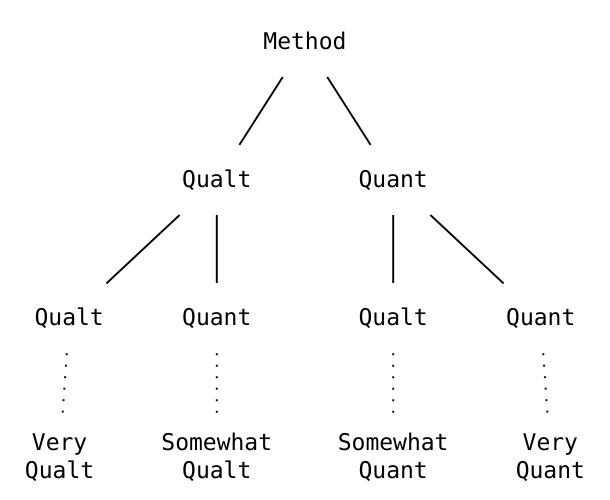
\includegraphics[width=6.35in]{img/fractal} 

}

\caption{Fractal Evaluation and Commensurated Scale. Adapted from Abbott (2011:11).}\label{fig:fractalp}
\end{figure}

Facing inwardly, they deploy value standards rather than
classifications. In their own field, scholars grant themselves moral and
aesthetic authority to judge the quality of content. In communicating
outside of their field, where they have no jurisdiction, assessment of
cultural items becomes value neutral, a mere matter of taste. Such
internal values may even be simple dualisms compared to the more
complicated disciplinary categories, but rather than creating simple
genre-like schemes they create scales of gradient evaluation.
\citet{Abbott2001Chaos} shows that these scales, for instance from
idiographic to nomathetic, are established by the accumulation of simple
judgments by separate individuals in the direct and often pairwise
comparisons of discrete works or authors. This pattern of evaluation is
chaotic and produces a fractal organization of content with only
approximate correspondence among judges. Though Abbott
\citeyearpar[14]{Abbott2001Chaos} suggests that these fractals are
irreducible to simple one or two-dimensional scales, it is likely that
the chaotic outcomes are collapsed into a reified commensuration
standard when facilities and rewards are distributed
\citep{Espeland1998Commensuration}.

Disciplines are much more like genres than the constellation of fields
and subfields that scholars may be accustomed to thinking with in the
course of their work. Genres function to the extent that they are
globally recognizable, that is, ubiquitous. Ubiquity means that all
members of a field regardless of status are able to learn enough about
the genre to make accurate classifications of cultural objects. This
does not mean that everyone will always necessarily be aware of all
genre labels, or that their classifications will always be accurate, but
it does mean that they will be able to learn the rules when it becomes
necessary. Subfield categories are not ubiquitous in this way; subfield
labels only become genre-like by restricting the reference group to a
more esoteric level. Whereas all members of a university, for instance,
may easily become aware of the discipline of sociology, written as it
may be on a building, only disciples of sociology are likely to become
aware of the subfield of conversation analysis. And while disciples may
learn the label, it takes some real experience with the content of the
discipline, if not necessarily the subfield, to understand that
conversation analysis is more qualitative than population research and
more quantitative than ethnography.

In this way the classification schemes are nested in a functional
hierarchy that shifts according to which role relationships are
activated in the field. The more fine grained distinctions among genres
are derivable from the collapsed fractal patterns. The highest level of
granularity one is able to discuss may be a status signal of where they
belong within a disciplinary stratification system. Furthermore the
interactional capacities of disciples are nested. Denizens of more
interior spaces in a subdiscipline, the spaces of fractal evaluation,
are always able to operate successfully in more granular interactions,
but the reverse is not true.

Everyone starts at the more ubiquitous level. It is only through
education or professional socialization that newcomers can learn

\begin{table}[!htbp] \centering 
  \caption{Classificatory Schema by Role Relationship} 
  \label{tab:role-schema} 
\begin{tabular}{@{\extracolsep{5pt}} llll} 
\\[-1.8ex]\hline 
\hline \\[-1.8ex] 
Accessibility & Schema & Ego & Alter \\ 
\hline \\[-1.8ex] 
esoteric & fractal evaluation & scholar & scholar \\ 
. & genre class & scholar & student \\ 
.. &  &  & publisher \\ 
... &  &  & archivist \\ 
.... &  &  & department \\ 
ubiquitous & discipline class & scholar & administrator \\ 
 &  &  & public \\ 
\hline \\[-1.8ex] 
\end{tabular} 
\end{table}

\hypertarget{kd-dq1}{%
\section{JSTOR Journals}\label{kd-dq1}}

I rely on the JSTOR digital archive which gives access to optical scans
of historical journals. JSTOR provides a title list of their journal
coverage \citep{JSTOR2018Title}. The coverage of journals in the archive
is very complete for those journals chosen for the database. As of this
writing JSTOR contained 4,224 different journal titles and 2,738
journals from 1,147 different publishers. The different journal counts
are due to some journals changing titles at least once.\footnote{To
  avoid over counting, title histories are collapsed into their most
  recent record, meaning all subsequent counts are out of 2,738. Even
  though one might expect disciplinary identity to change over time,
  JSTOR discipline labels do not vary within title histories. One
  journal--Scientific American Mind--lacked any discipline labels and is
  excluded from tabulations.} The JSTOR coding contains 79 subject
labels. These labels refer to eight superdisciplines under which may be
found 71 disciplines.

Most journals are given more than one discipline label, and the
superdisciplines are not marked as such in the database creating some
redundancy. For instance, a journal labeled as ``Sociology'' will also
be labeled as ``Social Sciences''. Most academics will be familiar with
whether a label is for a superdiscipline or a subdiscipline, yet for
outsiders or for skeptical insiders, the only clue is in the frequency
with which a label is applied. Counting labels, however, does not
unambiguously place a journal in one discipline or another because
journals may bear multiple labels, even multiple superdiscipline labels.

\hypertarget{network-mode-projection}{%
\section{Network Mode Projection}\label{network-mode-projection}}

To assess the size of the disciplines and to disentangle their
hierarchies it will be helpful to have a mutually exclusive labeling
scheme that draws on the JSTOR curators' judgement while simplifying it.
I rely on network methods to accomplish this labeling in a data driven
and reproducible way. In a network representation of journal discipline
labels, two journals may be said to be be related if they carry the same
label. In network terms this can be represented as a bipartite or
bimodal network. In a bimodal network there are two types (modes) of
nodes, a journal and a label, and ties can only be registered between,
not within, these modes. So journals are not tied directly to other
journals and labels are not tied directly to other labels.

Given any bimodal network, one may translate or project it into either
of two unimodal forms. In a single mode or unimodal projection of a
bimodal network there is only one type of node, in my case either a
journal or a label, but not both. The omitted type is instead
represented as a set of ties among the included type. Though the bimodal
network is a more elegant representation, it is technically necessary to
project it into one of its two bimodal forms to leverage network methods
that are designed with unimodal data in mind.

Using the list of subjects associated with each journal in the JSTOR
title list, I construct the bimodal \emph{journal-label} network with
journals in the first mode bearing ties to discipline labels in the
second mode. I then project the bimodal network into two unimodal
networks, one where journals are connected by ties equal to the number
of discipline labels they have in common, and another where labels are
tied by the number of articles carrying both labels. Call each of these
unimodal networks, the (\emph{journal-label-journal}) journal network
and (\emph{label-journal-label}) label network, a facet of the original
bimodal network.

Figure \ref{fig:mod-proj} illustrates the effects of network mode
projection on a random sample of 300 edges from the full JSTOR title
list network. The first panel illustrates the bimodal network where
journals are yellow dots and labels are blue dots. As an artifact of
sampling, most journals here are shown tied to only one label. In fact
this is never the case in the full network; as each journal has at least
one discipline and one superdiscipline label the minimum number of
labels is two, which is the median case accounting for 53.9 percent of
journals. The most labels any journal bears is 10, but these are
outliers with most journals bearing only a few labels.

\begin{figure}

{\centering 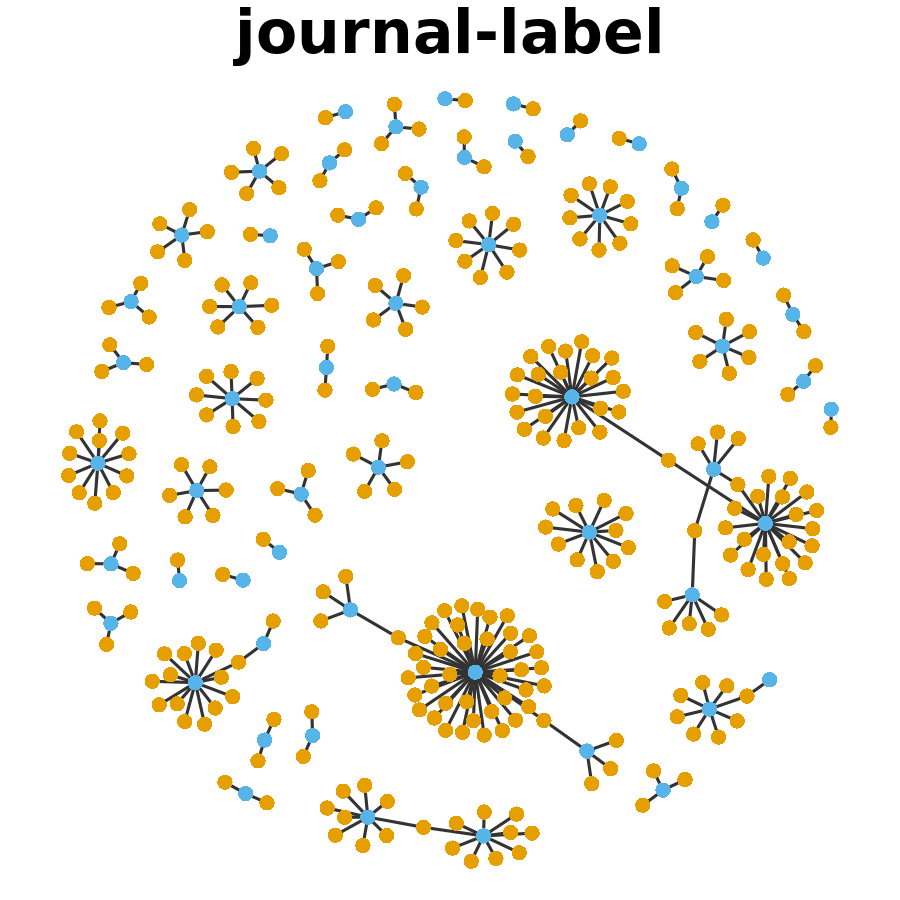
\includegraphics[width=0.3\linewidth]{ambrose_dissertation_files/figure-latex/mod-proj-1} 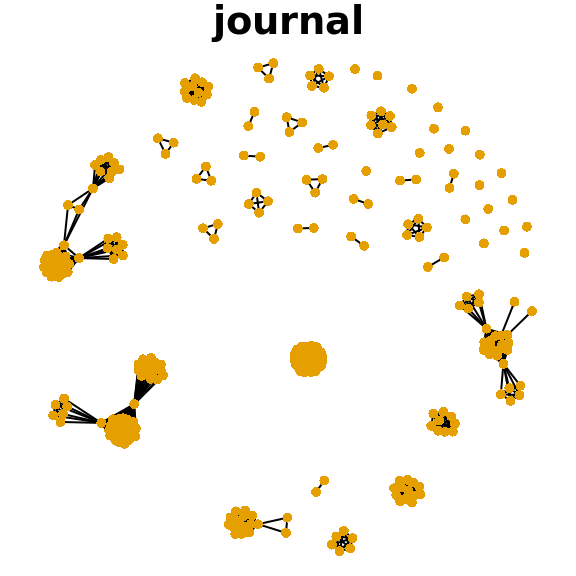
\includegraphics[width=0.3\linewidth]{ambrose_dissertation_files/figure-latex/mod-proj-2} 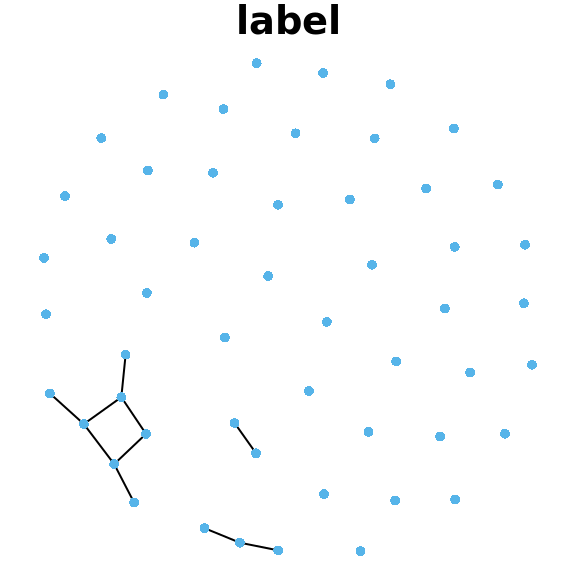
\includegraphics[width=0.3\linewidth]{ambrose_dissertation_files/figure-latex/mod-proj-3} 

}

\caption{Mode Conversion on a 300 Edge Random Sample of the JSTOR Title List Label Network}\label{fig:mod-proj}
\end{figure}

It is worth noting a few features of the unimodal projections or facets
illustrated in the second and third panels. First, unimodal projections
will always be made of overlapping cliques. Take the journal facet; each
journal bearing a particular label will be tied to each other journal
with the same label. Together they will form a clique, a subnetwork of
maximum density where all possible ties exist. Such cliques grow nearly
exponentially, as each additional journal with the same label joins the
clique and adds a number of ties equal to the former size of the clique.
In practice this means that very common labels like ``Social Sciences''
can easily dominate the unimodal projection of the network. Here the
weighting of edges becomes important; if two labels overlap because some
nodes bear both labels, then within the intersection of the two cliques
the ties may be treated as ``weighing more'' by adding the contribution
of each label separately. The exception is if the cliques overlap by
only one node, in which case they have a node but no ties in common.
Nevertheless using methods that take edge weights into account is a good
way to ameliorate the exponential influence of popular labels.

Second, though the unimodal facets of a bimodal network represent the
same data, each may have different characteristics especially in the
common case of a large population imbalance between modes. In the full
network there are 35 times as many journals as labels and each journal
sends multiple ties. This degree imbalance between the two modes may
mean that one facet is more dense than its inverse. Density is the
proportion of actual ties out of all possible ties. In Figure
\ref{fig:mod-proj} an imbalance may be observed where the journal facet
has many dense free floating or overlapping cliques and where the label
network appears to be mostly made of isolated labels save for the few
larger components. In the sampled network the journal facet is 10 times
more dense than the label facet. In the case of our full network, the
potential imbalance in degree distribution between facets happens to be
offset by the population imbalance itself. The densities in the full
journal and label facets are comparable, 26.2 and 27.3 percent
respectively, meaning that analysis will not merely hinge on which facet
is analyzed.

Third, unimodal projection has the effect of pruning what are sometimes
referred to as pendants, which are simply nodes with only a single tie.
Each of the isolates in the label facet represents a larger or smaller
number of journals, which may be observed in the different sizes of the
free floating cliques of the journal facet, yet no matter their size
they supply no information about interdisciplinarity. Because the
journal facet captures both size (of cliques) and relatedness (clique
overlap) it is a better representation of the information of the
original bimodal network. Its drawback is that it is larger and more
unwieldy to analyze. The label facet offers a simpler picture of
interdisciplinarity.

\hypertarget{network-community-detection}{%
\section{Network Community
Detection}\label{network-community-detection}}

Each facet described above will help answer a different question about
disciplinarity in the JSTOR archive as indicated by JSTOR's labeling
policy. I aim to resolve the uncertainty about which labels count as
superdisciplines and to reveal patterns of sorting not apparent in the
labels themselves. The rationale for doing this is to observe not the
choices of JSTOR coders, but the tacit judgement they likely used in
applying labels. I expect that the 79 fine grained labels belie a
simpler classification scheme of academic genres.

I will use two techniques, community detection and graph visualization,
to answer these questions. Communities are really subnetworks of high
density, or clusters. I operationalize disciplinarity as the presence of
clusters within the journal facet network. Community detection on the
journal facet will answer how many superdisciplines there are and the
size of each in terms of the number of journals belonging to it.
Visualization of the label facet will show how hard or soft are the
boundaries between disciplines and where the strongest interdisciplinary
relationships lay.

First, I use community detection to partition the JSTOR journals into
mutually exclusive disciplines. Community detection is a set of network
methods designed to expose clusters by grouping nodes together such that
they send more ties to members of their own group than they send to
members of different groups. There is a cottage industry around
developing algorithms and statistical models to learn an unobserved
community structure of a network \citep[see][ for an excellent
review]{Fortunato2016Community}. The choice of the right community
detection method is controversial especially for very large networks in
which cross-validation is difficult. Fortunately the network at hand is
small enough to validate directly which lowers the risks of choosing the
wrong method .

To wit I adopt the well-known Louvain method of community detection
based on hierarchical modularity maximization. \citep{Blondel2008Fast}
Modularity is a quality metric quantifying the trade off between
within-group and between-group ties. The modularity of any given
partition of a network into clusters is equal to the proportion of ties
that fall within clusters minus the expected proportion of within-group
ties if ties were distributed randomly. A division that is as good as
chance would have a modularity value of zero, a division better than
chance a value between zero and one, and a division worse than chance a
value between negative one and zero. \citep[8]{Newman2004Finding} Higher
modularity scores indicate a better sorting of the network into densely
tied clusters.

The Louvain method is a bottom-up agglomerative algorithm. The procedure
starts by assigning each node to its own community. Then, for each node,
it assigns the node to the neighbor's group that would most improve
global modularity. It repeats this until no move improves modularity.
This forms the first layer in the hierarchy. It then collapses groups
into nodes and repeats the algorithm on the condensed network, stopping
at the first level where there is no modularity improving move to make.
The first layer represents the most local, the last layer the most
global resolution of community structure.

Modularity-based methods are tried and true, and their drawbacks are
well-known. The Louvain method is not deterministic, as the outcome may
(but usually does not) depend on the ordering of the nodes in the
reassignment queue. However Louvain has several features that recommend
it. It is computationally fast on small to medium graphs and it is
freely available in network analysis software. It also gives a
hierarchical solution that provides the analyst with options to inspect
community structure at a range of local and global resolutions, akin to
a cartography of counties versus one of continents. Given the small size
of our network, a local resolution will not be overwhelming, so Louvain
is preferable to other methods that only offer the coarser global view.

Table \ref{tab:jclu-tab-sup} summarizes the results of applying the
Louvain method to the journal facet and taking the most localized layer
of the community structure. Learned labels are applied to the clusters
by assigning each the name of its most frequent label. Community
detection sharpens the boundaries between fields by placing each journal
unambiguously in one superdiscipline or another. This mutual exclusivity
is apparent by the sum of the given labels exceeding 100 percent.

\begin{table}[!htbp] \centering 
  \caption{JSTOR Journal Counts} 
  \label{tab:jclu-tab-sup} 
\begin{tabular}{@{\extracolsep{5pt}} lrrrr} 
\\[-1.8ex]\hline 
\hline \\[-1.8ex] 
Superdiscipline & Learned & Pct & Given & GPct \\ 
\hline \\[-1.8ex] 
Social Sciences & 790 & 28.9 & 916 & 33.5 \\ 
Humanities & 664 & 24.3 & 719 & 26.3 \\ 
Area Studies & 357 & 13 & 499 & 18.2 \\ 
Science \& Mathematics & 307 & 11.2 & 360 & 13.1 \\ 
Business \& Economics & 266 & 9.7 & 285 & 10.4 \\ 
Arts & 240 & 8.8 & 293 & 10.7 \\ 
Law & 84 & 3.1 & 132 & 4.8 \\ 
Medicine \& Allied Health & 30 & 1.1 & 52 & 1.9 \\ 
Total & 2738 & 100.1 & 3256 & 118.9 \\ 
\hline \\[-1.8ex] 
\end{tabular} 
\end{table}

The first finding is that of the 79 labels these eight form the top of a
hierarchy of superdisciplines. Area Studies stands apart and is not
subsumed under either Social Sciences or Humanities. Social Sciences
journals predominate due to JSTOR's initial focus in that area, even
without counting economics among them, and Science \& Mathematics counts
for a larger than one might think. Economics stands apart from the
Social Sciences, and indeed Business \& Economics marks the transition
from the larger academic journal space to the smaller professional space
of Arts, Law, and Medicine \& Allied Health.

The given labels do overlap and one can recover a picture of
interdisciplinary by clustering and visualizing the label facet. This
facet presents a simplified view. Recall that each facet represents the
same data, the difference being whether a journal or a label is
represented as a node or an edge, and that there is a population
imbalance in favor of journals over labels. The larger the population
the easier it is to partition into a greater number of subpopulations.
Conversely, because there are far fewer labels than journals, one would
expect the clustering to be less granular for the label network than for
the journal network. In fact there is only one less cluster--Law--which
is subsumed under Social Sciences.

\hypertarget{network-visualization}{%
\section{Network Visualization}\label{network-visualization}}

Figure \ref{fig:jclu-lnet} visualizations the relationships among
disciplines, where again the strength of ties is equal to the number of
journals bearing both labels. Here the label with highest number of ties
within its cluster becomes the category name of the cluster. That label
is then omitted as a node and is instead visualized as a color coding of
its cluster, reflecting the special status of the superdiscipline
labels.

Unlike traditional graph visualizations that are designed to be pleasing
to the eye, this one is drawn according to a statistical model called a
latent position or latent space model. It starts with a simple idea that
the weight of the edges (the number of journals carrying both labels) is
a count that follows a Poisson distribution. This distribution may be
modeled by log-linear regression where the logarithm of the mean of the
distribution is a linear function of an intercept term and covariates.
What is interesting about the model is that the covariate of interest is
treated as the distance between the nodes in an unobserved or latent
space. The distance is treated as negative such that as nodes get closer
together (as the negative distance increases) the count of the edge
weight between them increases (technically the logarithm of the mean of
the count increases).

It is an elegant idea, but estimating the model is complicated. The
distances are metaphorical, and to realize them requires positing a
euclidean space in which each node has coordinates. From the coordinates
the distances can be easily calculated, but knowing which are the right
coordinates requires a complicated estimation routine based on
optimizing goodness of fit between guesses of the coordinates and the
actual count data. The estimator begins with coordinates taken from the
conventional Fruchterman Reingold layout algorithm and uses Markov Chain
Monte Carlo simulation to converge toward the positions that optimally
fit the latent space assumption \citep[See][ for details of the model,
estimation, and software]{Krivitsky2008Fitting}. Even if the estimator
does not arrive at a perfect solution it improves upon a conventional
layout in the direction of meaningful, and not just pretty, aesthetics
thereby helping the viewer to avoid artifacts and perceive real
information about the network.

Another great feature of the latent space model is that it allows
additional terms to be fit alongside the latent distances. It is
possible to control for or net out the effect of nuisance terms like any
other regression. As discussed above there is a concern about the undue
effect of popular labels. I have already tried to remove the
superdiscipline labels from the label network, preferring to represent
them as color coded categories rather than nodes. Popular labels may
still remain, however, and due to the exponential growth of ties during
downmode conversion even a handful of them will have a disproportionate
influence on the global layout of the graph.

This degree distortion can be controlled for by what is called a
sociality term, which can be thought of as a measure of a node's
popularity. A sociality term is a score for every node that if positive
means a node is more attractive and if negative means a node is actually
repulsive of ties. When viewing the positions of a latent space model
also fit with a sociality term, the space will measure relatedness
without the effects of popularity.

Figure \ref{fig:jclu-lnet} plots the results of a latent space model on
the label facet omitting superdiscipline nodes. Figure \ref{fig:layouts}
plots the same in an animation comparing the latent space and
traditional Fruchterman Reingold layouts. I will interpret the substance
of the latent space layout below, but first I will comment briefly on
some of the differences between it and the traditional layout.

\begin{figure}

{\centering 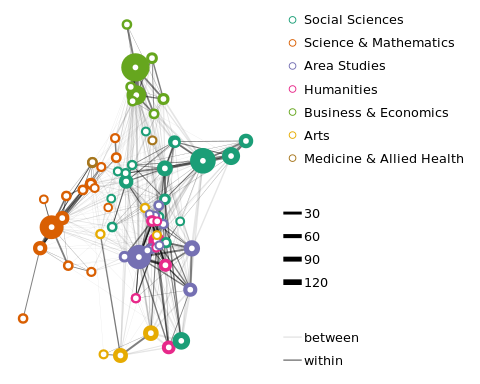
\includegraphics[width=0.9\linewidth]{ambrose_dissertation_files/figure-latex/jclu-lnet-1} 

}

\caption{Discipline Network in Latent Space.}\label{fig:jclu-lnet}
\end{figure}

\begin{figure}

{\centering 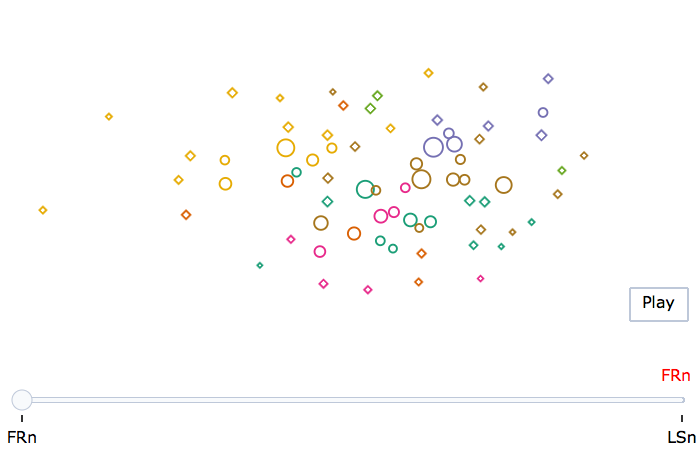
\includegraphics[width=0.9\linewidth]{img/layouts} 

}

\caption{Fruchterman Reingold and latent space layouts compared}\label{fig:layouts}
\end{figure}

In the animation nodes are hollow shapes to make their overlaps more
obvious. The size and shape of the nodes relates to their fitted
sociality: circles indicate attractive and diamonds repulsive nodes, and
the the larger the shape the more attractive and the smaller the more
repulsive. The layouts differ in two important respects. First the
global patterns are dissimilar. The latent graph has four discernible
arms. The traditional graph is a cloud that at first glance seems evenly
dispersed, however there is a prominent core periphery pattern, with
circles concentrated in the center and diamonds displaced in a ring
around them. Second, patterns of node proximity are distinct. In the
latent graph, nodes may share or almost share a center, indicating
structural equivalence. In the traditional layout concentric node
positions are algorithmically prohibited by a repulsion radius, with
apparent overlaps due only to the scaling of node size. The traditional
core periphery pattern is the consequence of the imbalance between low
and high degree nodes; by netting it out with the sociality term the
latent model makes it possible for minor disciplines to cluster around
the major ones to which they are anchored.

\hypertarget{results}{%
\section{Results}\label{results}}

Recall that the superdiscipline classifications are functions of their
underlying subgraph densities, hence we should expect them to be
clustered together in a layout that represents relatedness. For
convenience we will refer to the cardinal directions to locate ourselves
on the plot. The most prominent feature of the global patterns is the
appearance of two axes. From west to east is an axis dividing the
natural and the social sciences. From north to south is a more diffuse
axis dividing Business \& Economics from the Arts and Humanities. Though
it is tempting to interpret the south to north axis as artistic
opposition to profit, it is more plausible that they are each facing a
different side of the Social Sciences, which neatly bifurcates them.

\begin{table}[!htbp] \centering 
  \caption{Disciplines by sociality multiplier} 
  \label{tab:jclum} 
\begin{tabular}{@{\extracolsep{5pt}} lrrrr} 
\\[-1.8ex]\hline 
\hline \\[-1.8ex] 
Superdiscipline & Major Discipline & Soc. & Minor Discipline & Soc.  \\ 
\hline \\[-1.8ex] 
Area Studies & History & 9.4 & Irish Studies & 0.93 \\ 
 & Asian Studies & 4.35 & Latin American Studies & 0.86 \\ 
 & Middle East Studies & 2.96 & African Studies & 0.84 \\ 
 & American Studies & 1.5 & African American Studies & 0.45 \\ 
 & History of Science \& Technology & 1.38 & Slavic Studies & 0.22 \\ 
 & Jewish Studies & 1.07 & American Indian Studies & 0.2 \\ 
 &  &  & British Studies & 0.19 \\ 
 &  &  &  &  \\ 
Arts & Art \& Art History & 3.91 & Urban Studies & 0.6 \\ 
 & Architecture \& Architectural History & 3.49 & Music & 0.58 \\ 
 &  &  & Garden \& Landscape & 0.42 \\ 
 &  &  & Performing Arts & 0.31 \\ 
 &  &  &  &  \\ 
Business \& Economics & Business & 11.94 & Finance & 0.99 \\ 
 & Economics & 6.46 & Labor \& Employment Relations & 0.86 \\ 
 & Public Policy \& Administration & 1.68 & Development Studies & 0.76 \\ 
 & Management \& Organizational Behavior & 1.45 & Marketing \& Advertising & 0.72 \\ 
 &  &  &  &  \\ 
Humanities & Language \& Literature & 4.46 & Bibliography & 0.5 \\ 
 & Classical Studies & 2.72 & Library Science & 0.37 \\ 
 & Religion & 2.26 & Folklore & 0.36 \\ 
 & Philosophy & 1.5 & Film Studies & 0.2 \\ 
 &  &  &  &  \\ 
Medicine \& Allied Health &  &  & Health Sciences & 0.86 \\ 
 &  &  & Public Health & 0.7 \\ 
 &  &  & Health Policy & 0.34 \\ 
 &  &  &  &  \\ 
Science \& Mathematics & Biological Sciences & 9.09 & Mathematics & 0.88 \\ 
 & Botany \& Plant Sciences & 3.09 & General Science & 0.86 \\ 
 & Ecology \& Evolutionary Biology & 3.07 & Aquatic Sciences & 0.77 \\ 
 & Environmental Science & 1.7 & Paleontology &  \\ 
 & Zoology & 1.43 & Horticulture & 0.72 \\ 
 &  &  & Geology & 0.5 \\ 
 &  &  & Statistics & 0.49 \\ 
 &  &  & Technology & 0.44 \\ 
 &  &  & Engineering & 0.28 \\ 
 &  &  & Developmental \& Cell Biology & 0.19 \\ 
 &  &  & Astronomy & 0.04 \\ 
 &  &  &  &  \\ 
Social Sciences & Political Science & 10.26 & Geography & 0.82 \\ 
 & International Relations & 5.43 & Psychology & 0.64 \\ 
 & Archaeology & 5.16 & Environmental Studies & 0.63 \\ 
 & Sociology & 4.04 & Feminist \& Women's Studies & 0.58 \\ 
 & Peace \& Conflict Studies & 3.21 & Criminology \& Criminal Justice & 0.46 \\ 
 & Education & 3.15 & Social Work & 0.36 \\ 
 & Law & 2.08 & Population Studies & 0.27 \\ 
 & Anthropology & 1.45 & Communication Studies & 0.21 \\ 
 & Linguistics & 1.12 & Transportation Studies & 0.2 \\ 
\hline \\[-1.8ex] 
\end{tabular} 
\end{table}

While superdiscipline members are usually near each other, they do not
all bunch together in the same way. In the north Business \& Economics
is the most spherical cluster with its members much more strongly
connected inside than outside the group. By comparison Science \&
Mathematics is extended between two internal poles, with life sciences
pulled far to the west and statistics and mathematics interfacing with
other central disciplines. The Social Sciences are similarly extended
but with three poles: politics in the east, archaeology in the south,
and geography in the west. Area Studies, which subsumes history, tends
to closely overlap the Humanities with the exceptions of asian and
middle east studies to the east, which are situated between political
science and archaeology, American studies in the west, and the history
of science and technology, which is closer to its subject matter in the
west. Most of the Humanities is highly concentrated with the exceptions
of bibliometry and library science on one hand and classical studies,
which is close to archaeology, on the other. The arts is the most
diffuse superdiscipline; several of its fields are on the margins with
the exceptions of urban studies at the confluence of the Sciences and
Social Sciences and music as well as performing arts sharing the
interdisciplinary center with the Humanities and Area Studies. Finally,
the three disciplines in Medicine \& Allied Health are split between a
Science (public health, health sciences) and Social Science (health
policy) orientation.

There are several interesting cases of total or near structural
equivalence. Total overlap for major fields suggests extra
superdiscipline candidates, with biological sciences covering zoology
and history covering American studies. Considering only minor discipline
overlaps, the public health and health sciences labels overlap to the
point of redundancy, as do library science and bibliography. Near
overlaps between minor and major fields may indicate a theoretical
(major) applied (minor) relationship. This is expectation is confirmed
by the major law and minor criminology \& criminal justice overlap, and
contradicted by the major education and minor psychology overlap, where
the minor psychology field would be considered the more theoretical.
Interestingly, structural equivalence of fields in two different
superdisciplines occurs only once, with religion (Humanities) and Jewish
studies (Area Studies) tightly coupled.

A last topological feature of interest may strain the accuracy of the
model, but I lodge it as a problem for further consideration. Within
Area Studies there appears to be two differentiated fronts, a more
southerly line of ``white studies''--history, American studies, British
studies, Irish studies, and Slavic studies--and a more northerly line of
``brown studies''--American Indian studies, African American studies,
Latin American studies, and African studies, which also includes a spot
for feminist and women's studies from the Social Sciences. The distances
in question are very close, and model variability may reveal them to be
statistically insignificant. Even if they are significant their over
interpretation risks a narcissism of small differences.

\hypertarget{discussion}{%
\section{Discussion}\label{discussion}}

There are many stories to tell about a map that we trust to be an
accurate metaphor for closeness or relatedness in a cultural field.
Recall that statistically, the closer two nodes are the greater the
number of journals listing each as a subject category. The decision of
how the subject labels were applied was a policy decision at JSTOR using
an unknown procedure. Our interpretation of the map is affected by how
credible we think the archivists' decisions were. Without knowing about
their process, it becomes a matter of trust.

To begin with the weakest result, the purported fronts between white and
brown studies,

\hypertarget{gen}{%
\chapter{Genre and the Literature}\label{gen}}

\hypertarget{abstract-2}{%
\subsubsection*{Abstract}\label{abstract-2}}


In English the term \emph{genre} is a loanword from the
French term for \emph{kind}. As an analytical term in the social
sciences genre is a loanword from the humanities. The use of the term
varies greatly within and between disciplines. This study attempts a
metadisciplinary literature review of genre as a term found in a corpus
of JSTOR articles. I cast a very wide net by including any document in
English that includes the term genre in the title or abstract. The
resulting thousands of documents are ``read'' with the assistance of a
statistical topic model to classify documents into topics, that is,
strata of common vocabulary. I then perform content analysis on a
stratified sample of classified texts to compare their different uses of
the term genre. In an examination of the benefits and hazards of such a
distant reading approach, I outline a battery of diagnostics to examine
the validity of the topic model from both quantitative and qualitative
perspectives. Through a combination of machine distant reading and human
close reading, I arrive at a schema of five theories of the term genre.
In an argument for pandisciplinarity, I conclude with an analysis of the
logical possibility of new metaconcepts of genre that satisfy the
strictures of multiple disciplines.

\hypertarget{keywords-2}{%
\subsubsection*{Keywords}\label{keywords-2}}


genre, disciplines, computational text analysis, topic
modeling, content analysis, digital humanities, distant reading

\begin{center}\rule{0.5\linewidth}{\linethickness}\end{center}

In a motivation of some of the arguments to follow, I take a
metadisciplinary approach, which is to cast as wide a net as possible on
the term genre. In so doing I hope to test the tacit cultural assumption
that discipline-based decisions of relevance are valid, that is, that
when we exclude arguments from other disciplines we remove distractions
and focus on what is important. The alternative possibility is that we
are wasting intellectual resources, because to exclude important work
about our topic, even if it is codified in foreign terms, is to risk
ignorance and redundancy. The topic is genre and how disciplinary
boundaries form such that people using the same word nonetheless cannot
communicate effectively. They draw on different paradigms, which is to
say the term is not really the same term. What I hope to do is uncover
the knowledge contexts surrounding the terms, and map these contexts in
a way that enumerates the various communities of discourse and theories
constituting the term.

\hypertarget{genre}{%
\section{Genre}\label{genre}}

I take genre as a candidate explicans for the ability of scholars to
know what to read and what to avoid from the cultural archive. A theory
of genre will benefit from a review of the literature, yet to do so
would catch me in the conundrum of performing the phenomenon I wish to
explain. The genre structure of sociology should guide me to a
definition of genre, a statement that already presumes an ontological
difference and morphological relation between disciplines and genres,
namely that scholarly genres are not equivalent to scholarly disciplines
and that the former are located within the later. I will begin with an
unstudied attempt to tease out the relation of discipline and genre
before turning to a more rigorous, even empirical, treatment of genre as
a term in American scholarship.

Genre is a loanword from French. The origin of the French-Latin word
``genre'' and the English-German word ``kind'' both mean membership by
inheritance of innate class characteristics, archaically by presumptive
blood descent within a family, race, or nation. In common English it is
restricted to mean a broad category of art, especially literature and
music, and some but not all other cultural fields (e.g.~baseball is not
a genre of sports). As a term in scholarship, genre may be an observable
phenomenon, a conceptual component of a theory, or a conflation of the
two. In the social sciences genre is a specialty concept as in
sociology, while in the humanities it is ubiquitous especially in
cultural studies. Academics define and use the term differently between
and within disciplines.

Figure \ref{fig:ttsgnr} shows the count of mentions of the term genre in
the Google Books Ngram database for English terms
\citep{Michel2011Quantitative}. The trend exhibits the typical take-off
in publishing in the second half of the twentieth century. I apply
change point analysis, which detects significant differences in time
series data \citep{Matteson2013Nonparametric, James2019ecp}, to the
second difference of the trend, a measure of acceleration, to get clues
as to whether the trend is a single process or whether there are
inflection points. The first segment of the curve from 1899 to 1984
indicates a period of positive acceleration or quickening of the growth
trend. On average in the first period the rate of change from one year
to the next increased by a modest 13.3 occurrences a year. However,
during the period from 1985 to 2008 the rate of change, though always
steep, began to decline by an average of 238.3 occurrences a year. Like
a projectile that is simultaneously climbing and falling, 1984 acts as
launch point of precipitous yet unsustainable growth.

\begin{figure}

{\centering 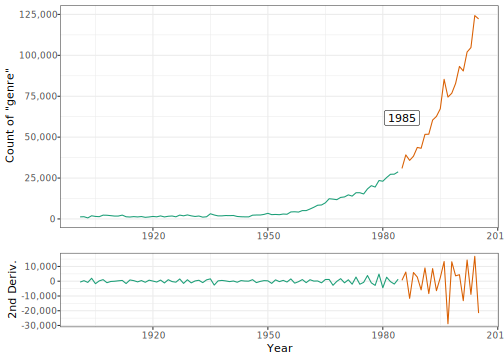
\includegraphics[width=0.9\linewidth]{ambrose_dissertation_files/figure-latex/ttsgnr-1} 

}

\caption{Absolute count of term "genre", 1901-2008.}\label{fig:ttsgnr}
\end{figure}

Figure \ref{fig:ttsgnr2} shows a similar trend but using relative
frequencies instead of absolute counts. Here ``genre'' is plotted as its
share of all terms in the corpus. This trend exhibits no inflection
point at 1984 that is statistically significant, and visually the trend
does appear the same on both sides. No other inflections points are
detectable due likely to greater year over year variability in this
series in the first half of the century, reducing confidence in any
estimate of a change point. To interpret this difference in statistical
significance between relative and absolute measures would indicate that
interest in genre continued to grow even within a secular slow-down in
the volume of texts that resembles the familiar S-shaped diffusion
curve. Alternatively, on visual inspection of the relative curve it
appears that indeed there is an inflection point, just one a decade
later in 1996. After this point the relative frequency seems to drop
rapidly, a change that would no doubt be picked up statistically after a
few more years of data and one that may in fact be located a few years
earlier than the peak suggests. Together these trends describe a career
to the term genre that has been strong for a century and that may now be
in decline.

\begin{figure}

{\centering 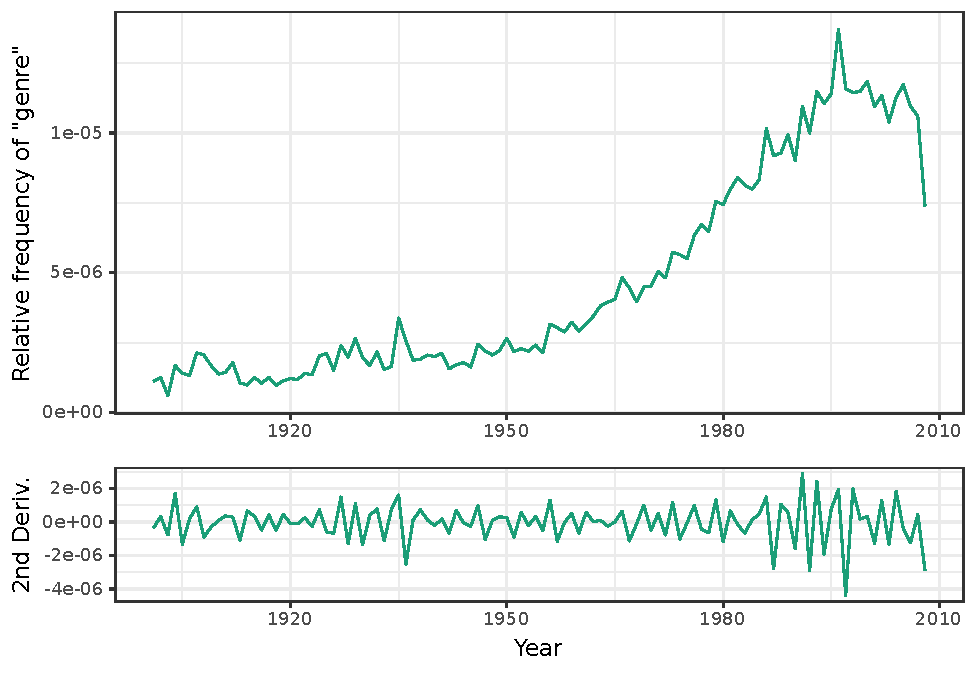
\includegraphics[width=0.9\linewidth]{ambrose_dissertation_files/figure-latex/ttsgnr2-1} 

}

\caption{Relative frequency of term "genre", 1901-2008.}\label{fig:ttsgnr2}
\end{figure}

Figure \ref{fig:genre-goog} gives an indication of what things the term
genre has been used to describe. It illustrates the frequency of terms
appearing in the Google Books Ngram corpus as the third term in the
trigrams beginning with ``genre of'' or ``genres of''
\citep{2012Google}. The size of the words is proportional to the total
frequency of the trigram in the English corpus, which spans centuries
from 1590 to 2008. The bias of the source--books--is clear in the
outsized importance of ``literature'' and ``writing'' which are followed
closely by ``music''. The next ten largest nouns are poetry, discourse,
fiction, art, autobiography, painting, film, romance, folklore, and
history. Ranked within that series would be several adjectives as well:
popular, science (fiction), historical, and literary. Each of these
terms refers to a field of concrete cultural products, with the
exception of ``discourse'' which is more abstract.

\begin{figure}

{\centering 
\includegraphics[width=0.9\linewidth]{img/genre-goog} 

}

\caption{Wordcloud of third term in 3gram beginning with "genre of".}\label{fig:genre-goog}
\end{figure}

Most items toward the top of the list are less popular (to write about)
art forms like television, dance, and theater. Toward the middle of the
list begin to appear adaptations of the term from the cultural to the
social context. These include practical fields like medicine and
journalism, political areas like law, government, and crime, and social
arenas like identity and protest.

\hypertarget{method}{%
\section{Method}\label{method}}

As I have said, the first consequence of eschewing disciplinary
limitations is to bloat the size of the ``literature'' on genre, since
no uses of the term would be excluded. An empirical approach to the
standard academic convention of a literature review will help reign in
the scale and complexity of the task. My aim, however, remains practical
rather than scientific. The methods need to be good enough to yield
results that offer something new above a traditional literature review
relying on library search and disciplinary wisdom about what is
important. This is not because a scientific approach is undesirable, it
is that it is not yet demanded of ``the literature''. Sociologists are
not expected to take a sociological orientation toward the history of
their fields. Rather the literature review serves the social purpose of
taking a position in a field of cultural production. It is a listing of
a roster of political support and rivalry, and an advertisement to
attract a desired audience.

To take an empirical approach to the literature review would be
subversive were it not the first function of disciplinary genres to
render atypical draws from the archive irrelevant. Disciplinary
subfields, genres, are credentialed by secret sets of references, and
most comers are held at the door. This in and of itself can be
subversive of even more arbitrary club rules, namely those of
educational pedigree, such that anyone willing to invest in a
presentation of the genre definition will be granted access to the
venues, if not the invisible colleges, of the subfield. To be admitted
to the arena is no guarantee of achievement within it, but it is a
start. Nevertheless, the scale of the archive will always supply entropy
enough to create a deterrent of flotsam and jetsam around subfields
composed of projects and persons who either never cracked the code or
who willfully eschewed it.

\hypertarget{distant-sampling}{%
\subsection{Distant sampling}\label{distant-sampling}}

The research strategy here attempts to parry the entropic tendency of
the archive by substituting human for machine limits. The methodological
premise of a meta-analysis of genre is that the Gordian knot of the
global cultural complexity of the archive can be cut by stratified
sampling. I use a large digital archive of texts, JSTOR, to represent
the whole of the academic archive. Though clearly a toy representing
only a fraction of all networked scholarly produce, JSTOR is large
enough to easily surpass individual cognition and compel the equivalent
types of complexity reduction facing any researcher approaching the real
archive via their local university library portal.

I use a simple term search of the keyword ``genre'' to define half of a
sampling frame.\footnote{TODO, I did not, but should take a random draw
  of the same size to serve as a control.} I could then take a simple
random sample of texts, analyze how each uses the term genre, develop a
classification scheme, and enumerate the different uses of the term.
Unfortunately, a small sample in a statistical sense may be larger than
a poor researcher can handle. 1,000 texts is not large statistically,
but it is huge from a content analysis perspective. What's worse, 1,000
texts may still exclude, by random chance, small subcultures of the
term. Stratification within a more or less global sampling frame
resolves this issue by delineating those subcultures so none would be
left out.

Alas, the JSTOR digital archive lacks subject labels at the article
level, though it does include them for book chapters and for journals.
While not foolish, inheriting a journal label to the articles included
within it may be a coarse approximation if within-journal content
variation exceeds between-journal variation. We can use text analytic
classification methods to cluster articles directly and discover latent
groups of articles, and in so doing we can have an independent standard
to compare to the discipline labels given to journals. It is an open
question whether such methods align with what we have discussed above as
disciplinary and subdisciplinary groupings, for us whether regularities
in vocabulary correspond to regularities in the meaning of the term
genre. If they do not, then the study will only be a stop en route to a
true census of the uses of the term genre, and the contribution will be
to have interrogated the quality of the methods used, though this would
be a small consolation indeed! Even so, for a new method to claim to be
able to improve on conventional wisdom, I behoove myself to proceed
methodically.

The choice in computational text analysis (CTA) about how to represent
texts as data hinges on whether word order is preserved. The older and
more tested approach is to not preserve word order. The name given to
this ``bag of words'' format reminds one of its inelegance. A bag of
words is a frequency table for each document counting up the number of
times particular words are used, a representation that effectively
reduces a text to its vocabulary. It is the analyst's crude operational
decision to treat vocabularies as indicators of meaning, but social
scientists conventionally insist on cross validation via qualitative
analysis. While the ambitions of computational text analysis may start
with a replacement of, for instance, the standard literature review, the
conventional distrust, at least in sociology, of mathematical models of
text makes CTA more of a sampling method than an analytic method. The
study will culminate in a reading of texts, albeit one that is different
than traditional qualitative analysis because the CTA researcher
welcomes the introduction of interpretive bias from an understanding of
the mathematical model before, during, or after the texts are read. In
the game of ``choose your influence'', CTA is one choice while
disciplinary wisdom is another.

There are two types of classification methods in text analysis, direct
document clustering and topic modeling. Direct document clustering
treats the bag of words as a vector space and calculates distance or
similarity metrics between documents, which are then clustered. In a
topic model, the relationship between documents is mediated by an
unobserved but latently modeled representation of their content;
documents are similar because they are formed from the same topics.

Whichever approach one takes, and both may be used, recall that the goal
is to organize the texts into strata for the purpose of stratified
sampling. We said that we wish to typify and enumerate the different
uses of the term genre. By qualitative analysis, we could read every
text in a simple random sample and come up with a theory of the use of
genre in that text. The demerits of this approach are several
\citep[c.f.][5]{Nelson2017Computational}. It would take longer than we
want even for too small a sample. We are not humanists and have not been
trained in text analysis (this will hound us no matter what). Fatigue
will set in, and accuracy and consistency will suffer. We may limit our
set of theories to spare us the agony of complexity. It will be hard to
reproduce our results. There may be path dependency with a different
reading order producing different theories. On the upside, we would be
more educated for it.

Instead, we will stratify the sample, and it is in the configuration of
the strata that much of the work will be done. The strata impose upon
our interpretation of the texts the assumption of sameness.

\hypertarget{no-cigar}{%
\subsection{No cigar}\label{no-cigar}}

The popular yet maligned distant reading approach taken by digital
humanists \citep[e.g.~][]{Moretti2005Graphs} is being taken up with
gusto by social scientists who are less skeptical of quantitative
methods \citep[e.g.~][]{DiMaggio2013Exploiting}. Following Nelson
\citeyearpar{Nelson2017Computational} I employ a quantitative analysis
of texts not to replace human reading with machine reading but to
support reproducibility in traditional qualitative content analysis.
While CTA makes it possible to dispense with reading altogether,
knowledge, understanding, and the cultural logics of
arguments--especially their ontologies--are still only obtainable by
reading primary texts, closely or not. The most radical interpretive CTA
method would involve deep neural net supervised machine learning, which
may be able to predict how a particular human reader would classify a
text without their needing to read it, though this has never been
demonstrated. What I gain from CTA is guidance in answering the question
of what to read, and perhaps in what order to do so.

As we know, the question of what to read is answered institutionally for
scholars already by way of canon, curriculum, word of mouth, and digital
reference term search services. These are their own forms of distant
reading, because they each make obsolete the archaic image, true of
figures like Weber, of a scholar buried in library stacks reading
everything they come across (and so it has been said of Weber,
forgetting nothing).\footnote{What a scandal it would be if Weber's
  lionizers discovered that he had only read text indices! Surely they
  would bury such a fact. But the point would remain that even if a
  scholar were able to consume an entire corpus, the sheer scale of
  contemporary publication is now beyond even a genius's capacity.}
These contemporary shortcuts are historically arbitrary, but what is
important is first that they serve the function of reducing the
overwhelming cognitive complexity of published scholarship, and second
that they structure that reduction in the same way for all scholars. An
arbitrary reduction needs to be consistent to act as an infrastructure
for subdisciplinary scholarship, otherwise scholars would find
themselves located in different literatures.

If distant reading is a criticism of close reading then it has a big
hill to climb especially among humanists who are trained to deal very
carefully with texts. In the social sciences a type of customary distant
reading is that of ritual citations, those that have developed a meaning
that may be oblique to their content or at odds with the intentions of
the the original authors. A ritual citation is simply one that is cited
but not read, but also one that is so often used that its socially
acceptable usages are known from other secondary accounts. For all the
lack of due diligence in the use of ritual citations, their socially
understood meanings are better than the thoroughly perfunctory citation,
those included because they were returned by a digital reference service
and never read by anyone.

What are the social patterns of the traditional literature review are
topics for the sociology of knowledge and science and for the
information sciences. This is not the task of the current study. What we
take from the traditional approach is the consequences of excluding
large segments of intellectual history. What CTA makes possible for the
first time is a nonarbitrary, inclusive analysis of \emph{all} content
in a digitized corpus. It will not necessarily be a good analysis, but
what it will lack in quality it will make up for in coverage. A CTA
approach to the literature review will at least make clear what lacuna
would be left by the traditional approach. They also reduce the
potential idiosyncrasy of a particular author's literature review
because, unlike a personal reading, a CTA model can be communicated
precisely.

Of course the cognitive limitation of how much any scholar can actually
read and understand remains. There will be an exclusion mechanism no
matter what, therefore a chief assumption of a CTA literature review is
that corpus segmentation is both possible and that some reduced form of
reading, some sampling procedure, can be said to be representative of
the unread portion in each segment. These representative texts will be
subjected to a close reading, but their interpretation will be
generalized to unread documents. Hence I call this a ``no cigar''
approach to reading, as in ``close but''. If on the contrary to the
assumption no two snowflakes are alike, then the enterprise of knowing
more than we have before is fraught, and CTA becomes yet another
arbitrary reducer.

What is worse, or perhaps better, is that there is reason to believe
that idiosyncrasy itself is an historically variable feature of
disciplines. If institutional isomorphism has proceeded to some high
level in contemporary disciplines, then the assumption that reading the
bellwether texts is as good as reading the entire herd may hold. If this
is true, however, it raises as many questions about the process of
institutionalization in cultural production as it answers about the
potential to learn truer versions of intellectual history.

\hypertarget{topic-models}{%
\subsection{Topic Models}\label{topic-models}}

We have referred generically to computational text analysis, and now we
can discuss the topic model as our technique of choice. There are many
ways of estimating a topic model (e.g.~the famous Latent Dirichlet
Allocation (LDA) estimator) but the model itself is simple. It is a
latent variable model that decomposes a document-by-term matrix--in
which every document is represented as a frequency distribution over
every term appearing in the corpus--into two unobserved matrices:

\begin{itemize}
\tightlist
\item
  a topic-by-term matrix, and
\item
  a document-by-topic matrix.
\end{itemize}

Topics are directly represented by they topic-by-term matrix. A topic is
a probability distribution over a vocabulary. To draw on a topic means
to choose vocabulary as a random draw from this distribution, where
words with higher probabilities will be chosen more often. In the case
of genres we might imagine a topic about film and a topic about music.
Some words may be important (highly probable), to both topics, such as
the word ``genre'', while others would be distinct, such as the words
``movie'' (probable for film but improbable for music) and ``band''
(vice versa).

Note the usual distributional bait-and-switch of categorical statistical
analysis, where observed count data are operationalized as the outcomes
of unobserved probabilities. The probabilities are what will be
estimated, not the counts. The importance of this will be explored in
the sections on estimation and diagnostics, but suffice to say that the
differences between probabilities and counts encapsulate many of the
difficulties applied researchers encounter when using topic models.

Given topics as term distributions, a document can be represented not as
a distribution over terms, but as a distribution over topics. The topic
mediates the relationship between documents and terms. In order to
generate diction for a document, all that need be understood is the
ratio of topics out of which it is composed. This is sometimes explained
as a generative mechanism; to ask what word will be chosen next in
composing a document, one first samples from the document's own topic
distribution to decide which topic the word will be drawn from, and
given that topic, one then samples from the topic's word distribution to
decide which word will be included in the document. A document's topic
probabilities also create the expectation of how many words are
attributed to each topic. A document with topic probabilities .7 from
music and .3 from film would be expected to be 70 percent about music
and 30 percent about film, making for a parsimonious albeit reductive
description of document content.

It is important not to overinterpret a topic model. To describe a topic
model as ``generative'' implies that it explains how documents are
written. Such a generative metaphor reveals the absurdity of a topic
model as a representation of writing. Not to mention the fact that
punctuation tends not to be represented (though it could be), the terms
chosen would be in a random order incapable of making meaningful
sentences. Hence it is best to avoid the generative metaphor as an
explanation of texts. If topic models touch on the generation of real,
meaningful documents, it is only in a very limited sense. What the topic
model really represents is how vocabularies are organized to condition
an author's diction. A vocabulary can be thought of as an infrastructure
of meaning more trivial than grammar or syntax and much more trivial
than concepts or ideas. A topic is a simple list of words that is known
or knowable across all authors in a field. Topics do not tell stories;
authors tell stories in part by making diction choices that are
conditioned by topics.

From a sense or meaning making perspective topics are trivial; this is
because so little is known about what an author says by knowing the
topic or even the term distribution of a document. What topics are
useful for, however, is the segmentation or cartography of a corpus.
Topics are really a global feature, perhaps a cultural feature, of a
corpus of texts that is itself meaningfully selected. If indeed a field
of texts is oriented to common if not always overlapping vocabularies,
then topics can represent this well.

A topic model could be posited based on the domain knowledge of an
expert, and this would be a form of estimation. The practical value of
statistical topic modeling is that the unobserved topics can be induced,
with a raft of statistical assumptions, directly from the observed
document-by-term matrix to arrive at a model with the features just
described. An estimated topic model will contain several other
parameters filling in assumptions necessary to make it possible to
identify the unobservable topic probabilities in each of the two
matrices of the model. For instance, in LDA models the concentration
parameter commonly called alpha makes an assumption about how many
topics tend to comprise each document. Alpha values close to zero make
it very likely that documents are composed of only one topic, while an
alpha value greater than one increase the chance that a document will be
decomposed into several topics. Alpha equal to one creates no tendency,
so concentrated and diffuse mixtures are all equally likely to occur. It
would behoove a researcher to make an informed decision about this
parameter, yet software often sets an arbitrary default that the user
may or may not be fully aware of.

\hypertarget{choosing-k}{%
\subsubsection{Choosing K}\label{choosing-k}}

Finally, topic models require the analyst to choose the number of topics
K. The approach we take to guiding this decision is not to expect one
correct specification of K but rather to see it as a changing
resolution. A K=2 model usefully bifurcates the sample and is not simply
wrong because it is too restrictive. As K increases we expect the
samples to continue to divide as new parameter spaces become available
to partition the sample. While this is not strictly a hierarchical
design, since each K model is fit independently, we should expect to see
aspects of hierarchical topics as well as some degree of stability in
the relationships among topics.

Between model cross-validation means that document and term groupings
should be relatively stable as K increases. The document overlaps
between, say, a three topic model and a four topic model should not be
random. By graphing the document overlaps between pseudo hierarchically
organized models, it should be clear which topics are the most stable
and which are constituted partly by chance or by spurious association.
An ensemble approach would then recommend itself; if the content of a
topic is stable across different specifications of K, within limits,
then we should have even more confidence in that topic.

When parameter space is limited the content with the strongest signal
will come to define the topic, but the document by term vector will be
contaminated with content that would be separated given more space. For
sets of documents that are constituted by multiple true topics, we
expect to see splitting of larger topics as the resolution increases to
meet the real diversity. Hierarchy will reveal itself as topics with
stronger topic signals subsume weaker ones until K reaches a point where
there is enough space to separate them. On the other hand, in the
classic trade-off between variance and bias, where K overshoots the true
number of topics, we expect to see random splitting and possibly ``dust
bin'' effects where spare topics allow larger topics to prune their
weaker term associations. Indeed dust bins may appear even before the
true K is reached. Where the term proportions explained by topics are
very unequal, it may pay during estimation to treat a true smaller topic
as a dust bin for a larger topic, because the optimization gains of
clarifying a larger topic may be greater than the losses of confusing a
smaller one.

Another interesting feature of this approach is that it shows when and
how topics are able to appear given the parameter space constraints. We
expect the most dominant topics, those that appear at low K and remain
stable as K increases, to derive from vocabularies that are both
distinctive and used often. The content with the strongest signal will
be ``FREX'' terms, terms that are both frequent and exclusive
\citep{Bischof2012Summarizing}. Frequent means they have high counts in
the overall corpus either due to occurrence across many texts or to very
large counts in a few texts. Exclusivity (or monosemy, the opposite of
polysemy) means that terms co-occur with an invariable set of additional
terms. Exclusivity is related to the notion of anchor words that are
maximally exclusive, appearing in only one topic, but likely very
infrequent.The exclusivity of terms relates to the separability of
topics \citep{Arora2018Learning}, while the topic frequency of terms
relates to the topic's contribution to explaining global corpus
frequencies, that is, to maximizing model likelihood during estimation.

It should be possible to predict a priority for topic emergence as
models increase parameter space for topics. First, we expect topic model
estimators would be very tuned to picking out even a handful of texts
written in a different language than the main corpus, as terms within
those documents would be both frequent and exclusive. We should expect
technical jargon to also send a strong signal for it's high exclusivity.
Indeed, these special vocabularies are salient for both humans and
machines for the same reason; they are easy to disassociate from the
rest of the text. The priority, however, for the estimators will be to
explain global term frequencies, so jargon will likely be behind
frequent terms that appear across multiple topics, as in the case of
polysemy or the more common case of simple language ambiguity. Trailing
the pack and the last to emerge will be, as we have discussed,
idiosyncrasy.

Let us remind ourselves of what badness means, because a bad model in a
statistical sense may very well be the correct model for the analytical
purpose of the researcher. A human reader with an interpretive goal in
mind can be quite apt at scanning text content and ignoring what she
finds to be irrelevant. Some of this seeming irrelevance has to do with
the syntactic structure of language, while others a reader knows by
experience to be elements of style and rhetoric in their field. The
interpretive goal becomes like a flashlight that darkens much more
content than it illuminates.

While human readers tend to make sense of only small portions of texts,
the machine is not so lucky as to have the human capacity for selective
ignorance. The topic model estimator sees and makes sense of everything
at once. This is sometimes at cross purposes to the researcher's hope of
complexity reduction, because in interpreting the model rather than the
text she will be told by the model that something is important even if
she would have easily ignored the same context in the natural setting. A
topic model that is both correctly specified and accurately fit on a
large corpus will likely have dozens or even hundreds of topics. Such a
variegated classification scheme is likely to contain some topics that a
reader would consider to be redundant, for instance, because they are
about the same thing yet differ for an irrelevant stylistic vocabulary.
Many others will simply be irrelevant to her research agenda. The task
of sorting through the topics is supposed to be easier than sorting
through the original texts, yet the researcher is sure to find many
inscrutable lists of FREX terms in a that can only be understood with
reference to classified articles.

In the case that a correct model of vocabulary clustering is actually
too complicated to be helpful, the correct research decision may be to
deliberately underspecify the model. We can imagine the real topics as
guests standing in a line of priority, and the model is like a wedding
with a limited number of tables. The guests with the strongest relations
among them sit at the first table, the next strongest at the second and
so on until all of the tables are full. In their munificence the happy
couple still lets the remaining guests in, and what can they do but pull
up a chair at the tables where perhaps they already know one of the more
honored guests. However, if an additional table, or several, were to be
found, the crashers could look among themselves for close relationships,
even perhaps peeling away a priority guest, to form a separate group.
Prior to there being room, that group would be unrecognizably
distributed among several tables. The group would not exist, but the
individuals would, and they would find a seat somewhere.

Just as the arrival of wedding crashers at the tables does not alter the
identity of the core group that constituted them to begin with, a model
where K is set too low will serve to highlight those vocabularies that
send the strongest signals, even if the tails of these topic
distributions are contaminated by unidentified topics. From a frequency
and exclusivity standpoint the unidentified topics are the less
important ones. Smaller and less distinct groups will be occluded in an
underspecified model, and whether these are substantively important is a
theoretical decision.

\begin{table}[!htbp] \centering 
  \caption{Content priority across frequency and exclusivity} 
  \label{tab:frex} 
\begin{tabular}{@{\extracolsep{5pt}} lll} 
\\[-1.8ex]\hline 
\hline \\[-1.8ex] 
exclusivity & frequency &   \\ 
\hline \\[-1.8ex] 
  & low & high \\ 
low & 4. idiosyncrasy & 2. polysemy/ambiguity \\ 
high & 3. jargon & 1. foreign language \\ 
\hline \\[-1.8ex] 
\end{tabular} 
\end{table}

Indeed we may never expect idiosyncrasy to emerge as its own topic
except in the limiting case. Presumably K can be set so high as to
approach the saturation point of a topic for each document. In this
event topics that would otherwise appear in common may alter to
represent the uncommon parts of a document, and the topic would merely
reproduce the term distribution of a particular document. Thus there is
a transition from content in common to content idiosyncratic to groups
of trivial size and to individual texts in the limiting case. The model
is unable to ignore supposedly idiosyncratic content, and will thus find
a way to classify it among topics in common, effectively distorting the
term vector of those topics. There may be no objective point at which
the content in common is neatly separable from the idiosyncratic
content; indeed common content evolves only by idiosyncratic innovation.
An ensemble approach allows us to observe how particular content moves
among topics as parameter space opens up.

Finally, there may be hope that sparse model estimation techniques would
ameliorate some of the considerations above. Sparse model regulation,
such as those using the L1 or LASSO constraint, bias parameters downward
and thus may set trivial regression coefficients nearer to zero. Such an
approach may well fail to represent idiosyncrasy at all, which is either
a benefit or a hazard. Such a biased model would, by effacing the
idiosyncratic portions, yield topics representing only the common
portions of documents. This avoids what we have termed contamination at
the cost of losing information that we may care about. Thus for sparse
model techniques to be used responsibly document residuals would need to
be calculated to help recover the unmodeled portions of the texts. The
model diagnostics we explore below attempt to separate model parameters
into common and idiosyncratic elements, the difference being whether the
idiosyncrasy is located in the topic model or in the residuals.

\hypertarget{bias}{%
\subsubsection{Bias}\label{bias}}

Before documenting the data preparation below, it is important to keep
in mind several sampling and modeling considerations that tend to be
overlooked. First, idiosyncrasy is assumed to be unmodelable. A flaw of
traditional topic models is that, at one level, all documents are
generic. Originality exists only in novel admixtures of vocabularies
held in common. Vocabularies that are limited to trivially small sets of
works, be they idiosyncrasies of content or style, become sources of
bias to topic model estimators. Because idiosyncratic vocabulary is by
definition rare, it lacks both the mass of frequency and distribution
across documents to be reliably picked up as a topic. Indeed, if each
document were expected to contain some idiosyncrasy, then the number of
topics needed to catch all of the idiosyncrasy would be equal to the
number of texts in the corpus. Each document would then be a combination
its own idiosyncratic topic (of which it would account for 100 percent
of topic content) and a distribution over other topics held in common.
The real number of topics would then be K+N where N is the number of
texts and practically always much greater than K. Researchers would balk
at including such a large set of extraneous topics, while estimators
would both be strained by the greater parameters space and would collide
with hyperparameters designed to militate against estimating topics
distributed only over a single document.

The impracticality from a modeling perspective of representing
idiosyncrasy coincides with the undertheorized tendency among
researchers for extreme pruning of idiosyncrasy during data preparation.
A more parsimonious modeling solution would be to allow a single extra
topic designed to catch all idiosyncrasy. Yet this would tend to violate
the assumptions behind construction of the other topics for two reasons,
first because one topic would have significant distribution across all
documents and second because terms within the topic would never be
estimated together as they would really be a mixture of N uncorrelated
subtopics.

Idiosyncrasy tends to be pruned in a desire to limit the length of the
vocabulary to bring it within the bounds of computational power and the
chances of a successful parameter optimization. Depending on the task,
however, the researcher may not be so concerned with performance, and
may leave plenty of idiosyncrasy in the sample. What then is the effect
on the topic estimation of such idiosyncrasy, since the idiosyncrasy
must end up somewhere?

First, there will be a tendency to muddy the content of common topics
with the particular idiosyncrasies of the documents that happen to draw
on them. This in part explains the long, non-zero tails of topic by term
distributions, which are usually filtered out during post-estimation and
interpretation of the models. We would however expect them to corrupt
the error structure of the topic they contaminate, leading to suboptimal
estimates of the true terms in the topic.

Second, the document proportion of the contaminated topic will be
inflated in the contaminating document. After all, the idiosyncrasy of
the document was represented, erroneously, in the contaminated topic.
Because of the length of the term vector it is not difficult to imagine
the truly pathological case wherein the probability sum of the false
portion of the topic is greater than that of the true portion. In this
event, a document could be categorized within a topic due more to the
false content than to the true content, especially if the idiosyncrasy
was placed in topics randomly. Contrary to the effect of random error in
an explanatory variable in ordinary least squares linear regression,
which is to bias the regression coefficient downward, in a topic model
the effect will be to bias the topic probability of a document upward.

\citet{DiMaggio2013Exploiting} represent a typical albeit conservative
approach to topic modeling as distant reading. Their data preparation of
a newspaper corpus about U.S. arts policy in the 1980s and 1990s
resulted in 54,982 unique terms and 7,598 documents
\citeyearpar[582]{DiMaggio2013Exploiting}. This incredible
dimensionality in the term vector, which eliminated only stopwords and a
few hand-picked terms and did no stemming, represents a very
conservative approach to term filtering admitting to no performance
based truncation. They chose a model with 12 topics. Thus in a strict
interpretation of their 12-topic model, we are to believe that the
extreme idiosyncrasy of news, with all of its historical specificity, is
contained in a noise or junk topic rather than creating bias on the
estimation of the signal topics. With such a huge term mass to classify
and so few topics in which to do it, it is incredible to think that the
algorithm would alight on a junk topic rather than using that spot for a
signal topic. It is plausible that the noise (and so offensive a term to
those reporters trying to say something new!) is distributed across
signal topics rather than being safely tossed in the dust bin. To wit,
their choice of a low alpha parameter of 0.1, which assumes that each
document is generated from relatively few topics, makes it even less
likely that the estimator would spend precious parameter space on a
noise rather than on a signal topic.

\citet{DiMaggio2013Exploiting} attempt to placate statistical criticism
by substituting quantitative, statistical forms of validation for
qualitative cross validation of topics. This may be more treacherous
than the authors admit. Their analytical approach is:

\begin{enumerate}
\def\labelenumi{\arabic{enumi}.}
\tightlist
\item
  Fit the topic model.
\item
  Sort the topic by term vectors in decreasing order.

  \begin{enumerate}
  \def\labelenumii{\alph{enumii}.}
  \tightlist
  \item
    Split the fat head from the skinny tail.
  \item
    Interpret the terms in the fat head.
  \end{enumerate}
\item
  Sort the topic by document vectors in decreasing order.

  \begin{enumerate}
  \def\labelenumii{\alph{enumii}.}
  \tightlist
  \item
    Split the fat head from the skinny tail.
  \item
    Classify those documents in the fat head according to 2.b.
  \end{enumerate}
\item
  Interpret the documents according to 3.b.
\end{enumerate}

The sorting procedures are a typical low-hanging fruit use of the model.
Even though the model is a much simpler ball of string than the original
full text corpus, it is still a very complicated statistical equation
with, in this case, 12 * 54,982 + 12 * 7,598 = 750,960 estimated
parameters. Sorting the term and document vectors allows the analyst to
proceed from an interpretation of the strongest signals toward the
weakest, stopping when the author feels satisfied that the research
question is addressed. The assumption here is that the strongest
statistical signals are unbiased, that when parameters are converted to
ranks, and the ranks are converted to truncated lists of words and
documents, that those lists are correct.

The specter that I raised above applies to the document ranking more
than to the term ranking. A formal feature of topic models is that each
topic is composed of all terms in the corpus. Of course this is an
artifact rather than an intention of the model, as the goal is to
separate relevant from irrelevant terms in the constitution of topics.
Similarly, all documents are distributions over all topics, but this is
not (necessarily) the intention; again we expect an elbow in the sorted
topic document vector in front of which are relevant and after which are
irrelevant topics. Any concentration index, such as the Gini
coefficient, calculated on the topic term and to a lesser extent the
topic document vectors will show very high concentration, where most of
the probability is owned by a few elements.

We can test for some of these expectations of bias. A document's topic
assignment may be considered suspect if its term distribution from that
topic derives from the low and long tail of the topic, rather than from
the select high probability terms normally associated with the topic's
meaning.

\hypertarget{qualitative-cross-validation}{%
\subsection{Qualitative Cross
Validation}\label{qualitative-cross-validation}}

To be sure, topic model parameters may be biased by misspecification,
and if we are being fair, by the gargantuan task we ask of them. In part
because topic models, notwithstanding their decades of development,
remain difficult to validate statistically, and in part because educated
people scoff at the idea of machine reading, many researchers ultimately
rely on qualitative interpretation to evaluate model quality. Goodness
of fit means that topics pass a sniff test upon inspection. A list of
words either does or does not inspire a theory of meaningful content,
and this theory either is or is not confirmed upon inspection of
document with a highly ranked topic probability.

The same scholars who promote qualitative cross validation (QCV) would
presumably have bet on John Henry rather than the steam drill. The
arguments against the machine, which excels only at recognition, is that
it is a ham-fisted intruder into the delicacies of sensemaking,
semantics, and interpretation. Meaning operates very differently from
information namely by bringing grounding to the response to information.
One example of grounding is spreading activation, that when information
is presented to the mind by sensation, the mind responds by representing
not only a construct of the stimulus but also a network of constructs
adjacent in memory to the stimulus. Simply, humans see more than they
perceive, but machines cannot.

That machines are dumb because they recognize rather than interpret is
not entirely fair. In machine learning the analog to memory, be it
treated as semantic grounding or anything else, is mathematical model
representation, and the analog to learning is a Bayesian updating of old
models with new data. A machine seeing new data with an old model can
indeed see more than it perceives. At this moment in the era of
computational social science, however, researchers train models for the
first time on the data they wish to explain. It is theoretically
possible to communicate and transport models from past to present
researchers, however this is not done in practice for lack of
infrastructure and more importantly because social scientists rarely
study the same thing twice. Where data are ample it is possible to
simulate a history of memory for the machine using hold out techniques
where a model is trained on one sample of the data and applied to
predict another sample. Where the goal is to maximize prediction,
training and hold out samples are randomly selected. A different
approach \citep[e.g.~][]{Nay2017Predicting} involves selecting training
and hold out as a process in time. This is a closer approximation to
human memory, as humans always approach the present only armed with a
memory of the past. In this sense a time ordered model training process
may create the same kind of errors on new data that a social institution
would.

As clever as the time sorted hold out strategy is, it is unlikely to
outperform a supervised approach to model validation wherein human
judgements serve either as diagnostics or training materials for model
fitting. Human culture is far too expansive to be modeled by a computer
for no simpler reason than the data of human memory are always rapidly
lost and what is retained is selected for arbitrary historical reasons.
What makes the contest between John Henry and the steam drill
interesting in the modern era is the social problem of cultural
reproduction. Machines will outperform humans only where human history
is made more accessible to machines than to humans, which may be a join
function of the success of digital archiving coupled with the
deterioration of human education.

In the case of topic models, some advocates for the machine go so far as
to claim that the topic model actually recovers semantic context
\citep[578]{DiMaggio2013Exploiting} or what we have called grounding.
Semantic context is a more specialized notion than memory, and it refers
to the human capacity for reproducing common meaning. In language viewed
through a topic model a large collection of terms defines the topic
while only a sample of these terms will be observed in a particular
document. In this sense the topic model fills in missing information in
the way that meaningful interpretation does. This notion rests on a very
strong assumption, however, which is that information tacit in a
particular case is explicit in a different case, indeed a quorum of
different cases, and that the cases overlap enough to become included
under the same topic. With big variation in document length topic models
may take grounding, which is properly a community resource, arbitrarily
from the longer documents within a corpus thus giving them undue
influence over sensemaking. In real sociocultural interaction, a large,
exogenous influx of novel term associations would not determine meaning
at the margin. Real meaning has legitimacy enforced by interested
actors, such that deviant term associations are negatively sanctioned.
Topic models only learn from cultural expression and are ignorant of
social processes that condition expression. If novel terms are
associated in one text with a core of common terms found in many texts,
they too will be added to the topic. This is a corruption of the
grounding that would not occur in real life.

The estimation of grounding would seem to compete against the other
feature of polysemy, that a term may appear in multiple topics each with
a different context. How does the machine know that a particular term
distribution (document) is a case of missing grounding within the same
topic as another document, or is in fact a different topic with a
different context? Of course the machine knows nothing other than how to
maximize an objective function. Estimators are designed to start from a
more or less arbitrary guess and update parameters in the direction of
models that are more likely given the data. Indeed, it is the
hyperparameter choices of the researcher that often decide which
research approaches will win out. For example, the question of whether
or not a topic model detects polysemy is operationalized as topic
correlation and governed by the choice of the sigma prior, which
controls the diagonalization of the correlation matrix, where a
constraint toward low topic correlations prohibits detection of
polysemy. The current state of software discourages an understanding of
how hyperparameter tuning relates to a particular research agenda, and
this opacity to the method is a strong driver toward QCV.

Cheap computing does make grid searching across hyperparameter settings
possible, if not cost effective, but until this approach is usefully
automated it is safe to assume that models will be misspecified in an
unknown way, that the model is tuned in a particular arbitrary
theoretical direction that is unknown to the researcher. Why would one
believe that QCV would inoculate against the hidden bias imposed by the
model? To be clear, a biased model is one that will present a vocabulary
that \emph{does not} represent the text accurately. In the conventional
use of topic models, the researcher is eager to use the topic as a lens
that both arranges documents into relevant subsets (a particular draw
from the archive) and primes her interpretation of the documents content
by a suggestive list of terms. We wish to keep two forms of QVC error in
mind.

The first is classification error. Continuous document by topic
probabilities are interpreted categorically according to an explicit or
tacit threshold of classification. Explicitly, one could analyze the
global decay of topic probabilities and attempt to find natural
empirical separations at threshold values. More commonly, the tacit
satisficing criterion is met as one walks down the ranked list of
documents and eventually decides that they have understood the topic.
The error arises in the within-class generalization where classification
quality has degraded in a continuous fashion (and past the point reached
by our satisficed reader) yet such errors have been effaced by the hard
classification rule. In short, by understanding the bellwethers, the
researcher only partially understands the corpus and indeed only further
mystifies the poorly classified stragglers.

It will help to visualize the statistical situation leading to this
error. In the expected case of model misspecification, usually too few
topics, we should also expect an urchin shaped quality distribution
where on each topic spine are bellwether documents drawn out by their
strong signal to be representative of the topic. As one descends the
spine of each topic we will begin finding the poorly classified
documents collected on the body of the urchin. These documents are
representative of no topics, that is, equally representative of all or
several topics. For a misspecified model, it is possible that a
collection of these stragglers would be given a home in a model with an
extra spine, that is, new parameter space for an extra topic. But
without a topic to represent them, the analyst may make the mistake of a
false generalization from bellwether to straggler documents. Such
stragglers may even be halfway up the spine, assuring their
classification but for the wrong reason: bellwether documents achieve
their topic probability by virtue of words at the head of the sorted
topic by term vector, whereas stragglers achieve their lesser but still
above threshold topic probabilities from the meaningless long tail of
the topic by term vector. This long tail, we must recall, contains terms
that may have trivially small topic probabilities when considered
separately, but when considered together, because the term vector is so
long, their cumulative probability of the false segment of the vector
may rival in classification power that of the true segment.

The second is confirmation bias. Readers tend to skim and scan documents
more quickly and less carefully when they are told what they are about
ahead of time. It is natural for researchers to want to examine the
document by term vectors of the topics in order to understand the
results of the model and apply the findings to solve research problems.
These lists may be very evocative of theoretical assumptions and
practical expectations about the corpus, which has not normally been
read ahead of time. Theories of the meaning of the term lists are very
likely to establish confirmation bias in the reading of the texts. This
means that documents that have been classified by a satisficing or
threshold rule will be read differently with a theory of the topic in
mind than they would have otherwise. Confirmation bias means that the
analyst will have a tendency to focus on content that appears to conform
to the topic theory while discounting content that contradicts it.
Sometimes this will be warranted; after all, a feature of the model is
the ability to classify documents into multiple topics. In the
pathological case, however, the meaning of the document will be
distorted to fit the theory of the topic. A model that causes the reader
to misread a document is certainly not helpful, and the pull of
confirmation bias tends to be strong even when one is aware of it.

Fortunately we may adjust our research strategy to avoid each of these
errors. First, to ameliorate the effects of misclassification, a simple
concentration metric such as the Gini coefficient applied to the vector
will help discriminate between documents classified strongly into only a
few topics (highly concentrated probabilities) from documents that are
classified weakly into all (that is none) of the topics (unconcentrated
probabilities). To assess a particular topic classification it should be
possible to decompose the portion of a document's text that is estimated
to derive from a particular topic. That portion can then be scored
according to its weighted average rank of the terms actually contained
in the document, with poorly classified texts having lower scores. The
utility of this quality scoring is to shine a light on the yet to be
correctly classified texts, which may give an indication of when it is
warranted to increase the parameter space of the model, and which may
substantively reveal the less dominant (perhaps dominated) vocabularies.

Second, it is a simple enough procedure to forestall interpretation of
the topic by term vectors until after a direct inspection of documents
grouped by their topic classification. Indeed, this may promote a more
accurate theory of the topic since terms will be interpreted within
context.

\hypertarget{data}{%
\section{Data}\label{data}}

The JSTOR Data for Research service allows researchers to download
non-consumable versions of full text in very large samples up to 25,000
documents. We will use the JSTOR Data for Research service to download a
bag-of-words text corpus for topic modeling. I take the following steps
to develop a corpus:

\begin{enumerate}
\def\labelenumi{\arabic{enumi}.}
\tightlist
\item
  Search dfr.jstor.org using the query
  \texttt{(ta:genr*\ OR\ ab:genr*)\ AND\ la:eng} and requesting 1grams.
\item
  To cull documents for which genre is not an important term, exclude
  documents containing fewer than five variants of the term genre
  (1grams matching the regular expression \texttt{\^{}genr}: genre,
  genred, and genres).
\item
  Remove 1grams appearing fewer than three times, which often includes
  optical character recognition errors.
\item
  Remove 1grams shorter than three characters and longer than 25
  characters, again often OCR errors but also stopwords that will be
  removed anyway.\footnote{The Freudian ``id'' is an unfortunate
    casualty of this step, as well as some footnotes, endnotes, and
    captions containing small text where word boundaries were not
    detected during OCR and a series of words was concatenated.}
\item
  Remove 1grams longer than three characters that are all the same
  letter, often OCR errors but sometimes real, as in Roman numerals.
\item
  Compile baseline word counts for each document assuming that at this
  step the documents contain only valid terms, and no OCR errors.
\item
  Remove SMART stopwords.
\item
  Remove numbers.
\item
  Remove punctuation, except intraword hyphens.
\item
  Lemmatize or stem English words.
\item
  Remove lemma with fewer than three characters.
\item
  Aggregate 1grams defined by a single lemma and, for ease of
  interpretation, name the sum after the most common 1gram.
\item
  Remove terms appearing in fewer than 20 documents.
\item
  Remove documents that, after the above filters, have a word count of
  fewer than 500 words.
\item
  Remove documents that are identical in content to another document
  even if metadata differ, i.e.~reprints.
\end{enumerate}

The initial query returned 7,695 articles from 1,205 different journals,
as well as 6,485 book chapters from 4,427 books. After the above
processing steps, the sample was reduced to 3,547 articles and 2,797
chapters, or 6,344 total texts.

It is fair to ask what is lost during the pre-processing of texts. Many
are included in error due to JSTOR's internal translation of abstracts;
where ``genre'' is the French translation of the English ``kind'' the
text will be included even if the term genre does not actually appear in
the English title or abstract. While I do not carefully look at the
content of the excluded documents, assuming they were not texts that
made important use of the term genre, I do retain some information about
what components of a text were lost of those documents that were not
cut. This is a measure I call idiosyncrasy, or the proportion of terms
in a document eliminated during pre-processing. I call it idiosyncrasy
because the pre-processing condition was that terms would be eliminated
if they did not appear in at least 20 other texts. Texts that lost a
large volume of words to this filter are drawing on a vocabulary that
almost no other texts use. It would not be surprising if these were
ethnographic or content analytic studies of non English materials.

Figure \ref{fig:idi-hist} shows the right-skewed distribution of
idiosyncrasy. The median text lost about one tenth (10.19 percent) of
its words, while 90 percent of texts are within two tenths, and outliers
begin at about three tenths as can be seen in the boxplot. The 153 (2.41
percent of) texts above three tenths vary across a range as wide as the
rest of the distribution. The most idiosyncratic text, at 60.4 percent
of its vocabulary lost, is Welsh's ``Editorial: The Genre
Revival''.\footnote{www.jstor.org/stable/10.2307/27909026} The article,
from the journal \emph{Hebrew Studies}, is a single page introduction in
English to a 12 page essay reprinted in the original Hebrew. By page
count alone we would expect the idiosyncrasy to be 12/13 or 92.3
percent, which also illustrates how terms that are not in the Roman
alphabet may be discarded as OCR errors even prior to the idiosyncrasy
measurement.

\begin{figure}

{\centering 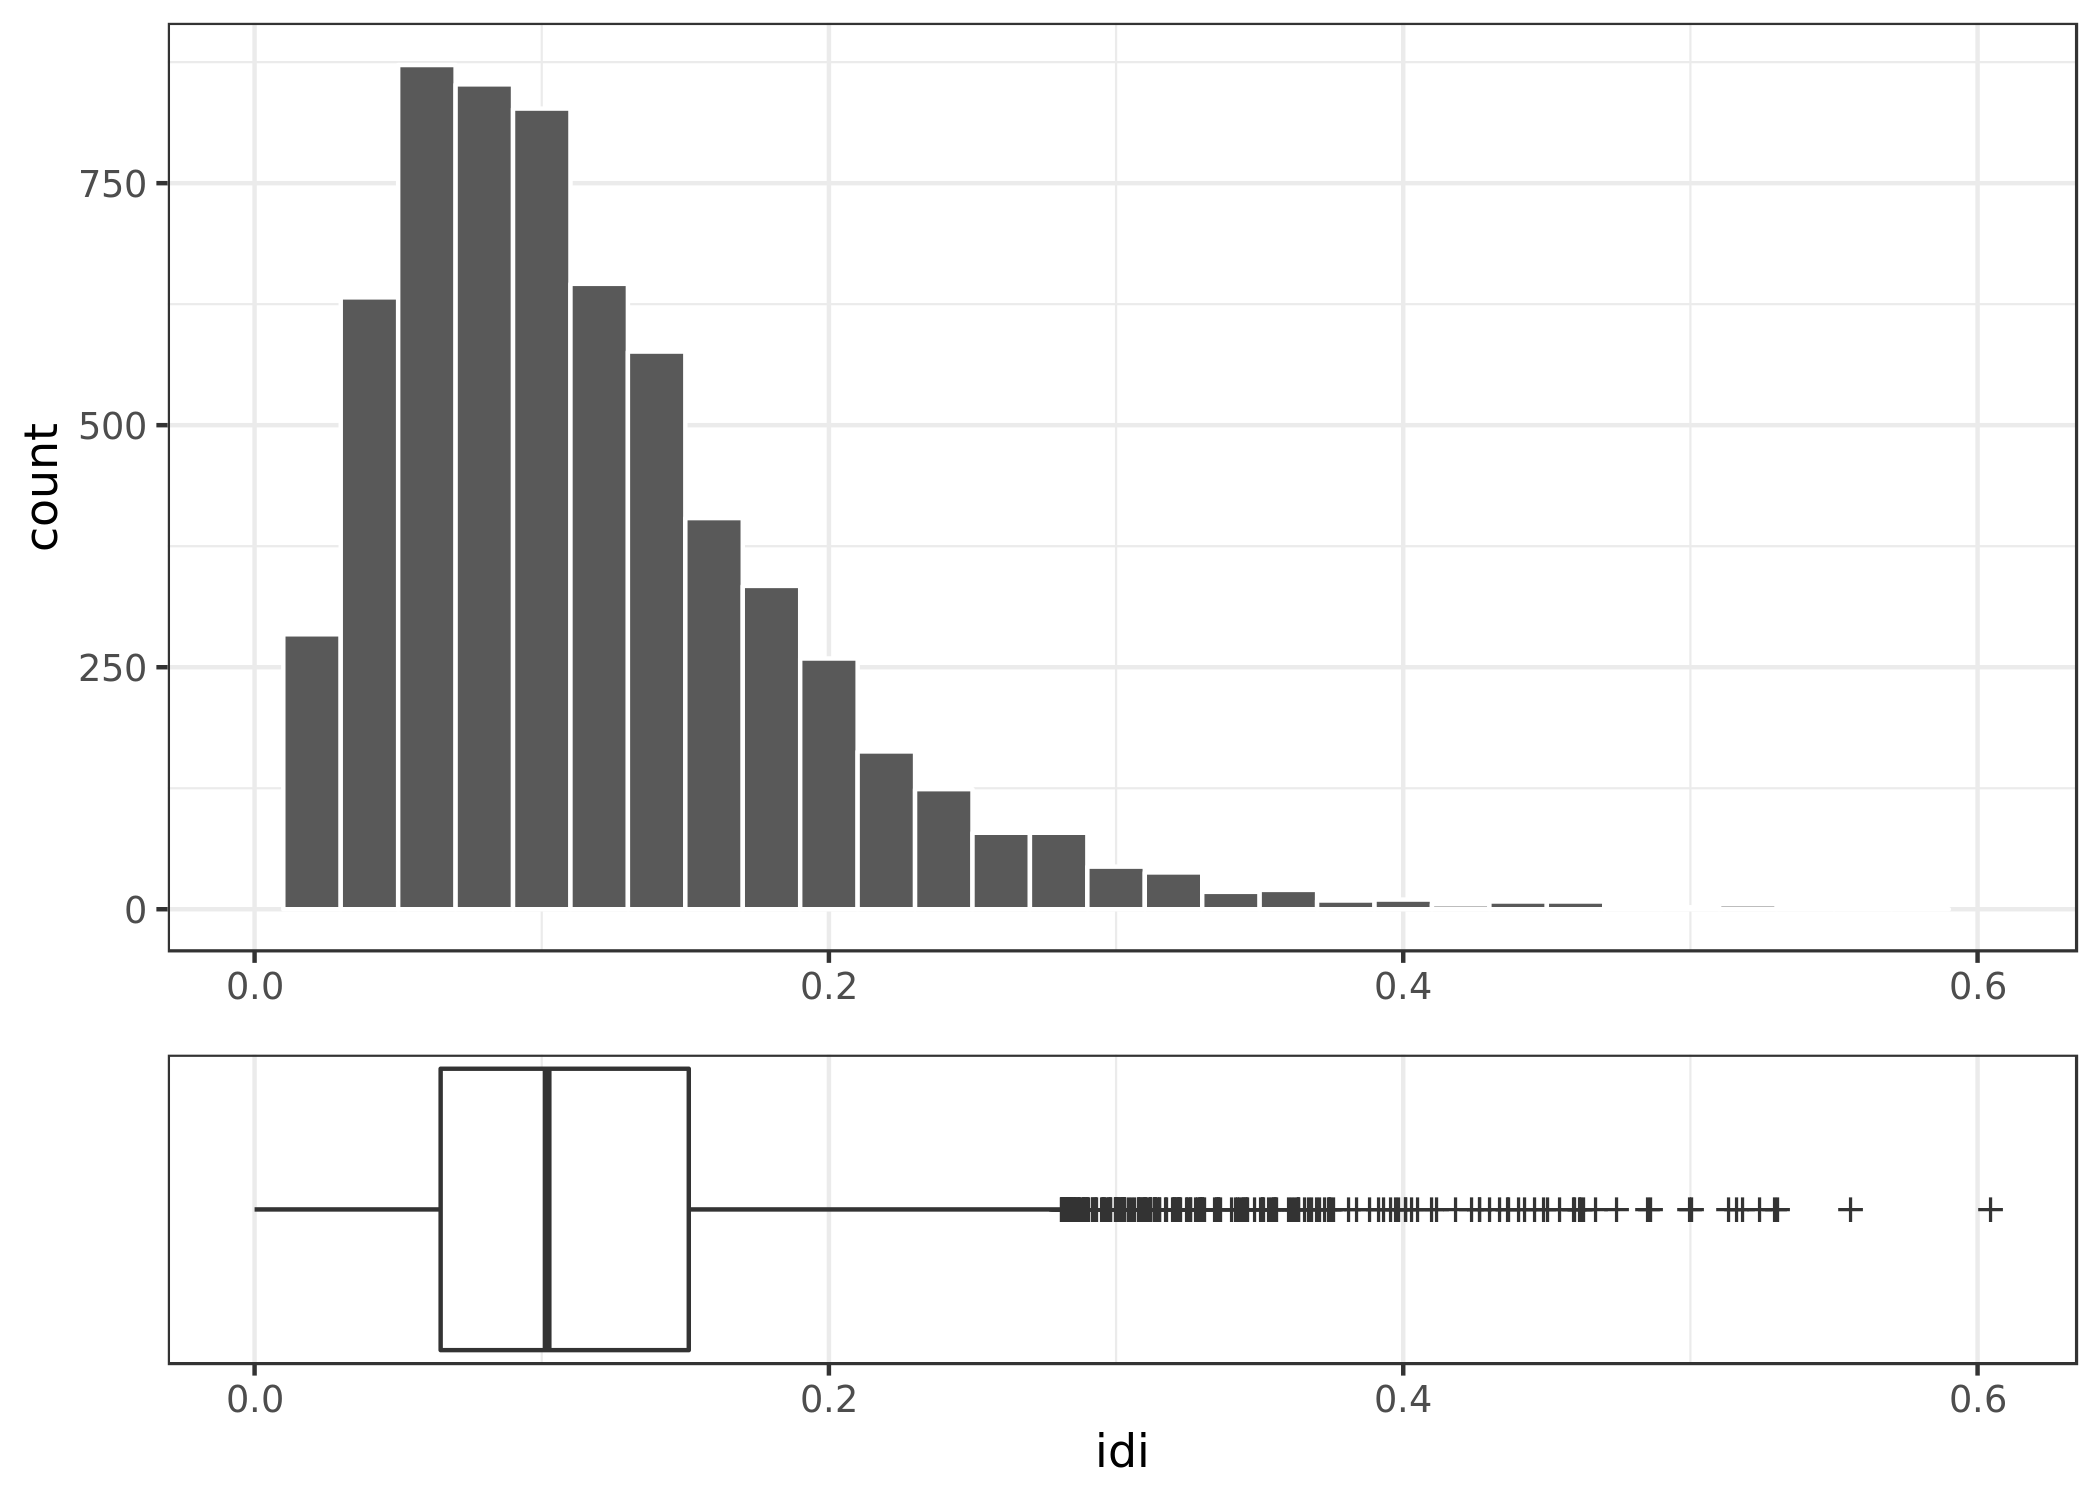
\includegraphics[width=0.9\linewidth]{ambrose_dissertation_files/figure-latex/idi-hist-1} 

}

\caption{Distribution of idiosyncracy, the proportion of document vocabularly dropped during pre-processing.}\label{fig:idi-hist}
\end{figure}

Figure \ref{fig:gp-hist} shows the logarithm of the count of the term
genre as a proportion of the total term count of a text. This
distribution is much more highly skewed but contains fewer outliers. In
the median text a genre variant accounted for about 6 in 1,000 terms,
while at the 90th percentile the rate is 27 in 1,000. 44 texts (0.69
percent) are outliers where one in ten or more words is a genre variant.
The text with the largest genre proportion, at 35.7 percent of its
words, is Welsh's ``Editorial: The Genre Revival''\footnote{www.jstor.org/stable/10.2307/43795866},
a single page introduction in a special issue of \emph{Literature/Film
Quarterly} on genres.

\begin{figure}

{\centering 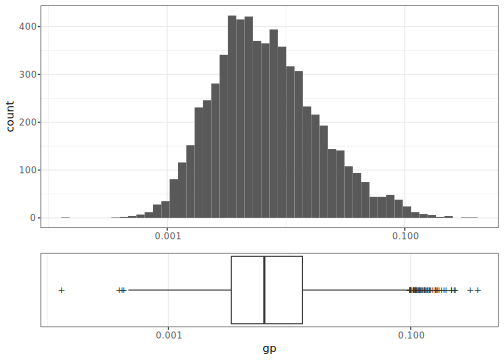
\includegraphics[width=0.9\linewidth]{ambrose_dissertation_files/figure-latex/gp-hist-1} 

}

\caption{Distribution of $log_{10}$ of the count of the term "genre" as a proportion of all terms in a text. Pluses indicate outliers.}\label{fig:gp-hist}
\end{figure}

\begin{table}[!htbp] \centering 
  \caption{Subject Distribution of Texts} 
  \label{tab:genre-jsubj} 
\begin{tabular}{@{\extracolsep{5pt}} lrrrr} 
\\[-1.8ex]\hline 
\hline \\[-1.8ex] 
Subject & N Percent & W Percent & N Rank & W Rank \\ 
\hline \\[-1.8ex] 
Language \& Literature & 20.29 & 26.96 & 1 & 1 \\ 
Humanities & 13.45 & 11.5 & 2 & 2 \\ 
History & 8.77 & 8.56 & 3 & 3 \\ 
Social Sciences & 7.19 & 5.46 & 4 & 7 \\ 
Area Studies & 5.57 & 3.55 & 5 & 6 \\ 
Sociology & 4.72 & 5.57 & 6 & 4 \\ 
Film Studies & 4.02 & 6.09 & 7 & 8 \\ 
Music & 3.83 & 4.84 & 8 & 5 \\ 
Arts & 3.65 & 3.33 & 9 & 9 \\ 
Education & 2.89 & 2.39 & 10 & 11 \\ 
Religion & 2.64 & 3.06 & 11 & 10 \\ 
Anthropology & 2.06 & 1.87 & 12 & 13 \\ 
Art \& Art History & 1.95 & 2.17 & 13 & 12 \\ 
Asian Studies & 1.77 & 1.18 & 14 & 15 \\ 
Performing Arts & 1.55 & 1.71 & 15 & 17 \\ 
Linguistics & 1.46 & 1.2 & 16 & 16 \\ 
Philosophy & 1.2 & 1.24 & 17 & 14 \\ 
Middle East Studies & 1.02 & 0.65 & 18 & 19 \\ 
Political Science & 1 & 0.88 & 19 & 21 \\ 
Other & 10.98 & 7.79 &  &  \\ 
Total & 100.02 & 100.01 &  &  \\ 
\hline \\[-1.8ex] 
\end{tabular} 
\end{table}

Table \ref{tab:genre-jsubj} enumerates the subject labels each text
inherits from its parent book or journal. JSTOR categorizes the volume
rather than each item of its contents, and volumes may bear multiple
labels. The count (N) of discrete labels as a percentage is listed first
and the table is sorted by that figure. In addition, to prevent double
counting of texts bearing multiple labels, each label is given a weight
(W) that is the inverse of the number of labels given to the text. The
top three, Language \& Literature, Humanities, and History, are the same
in each case, while Sociology, Music, and Area Studies are ranked higher
by weight than by count, an indication that Social Sciences frequently
co-occurs with other labels and is therefore down-weighted. This makes
sense as Social Sciences, like Humanities and Arts, is a meta subject.

``Subject'' is the name given by JSTOR as a description of content, yet
they also refer to ``discipline'', which as mentioned above is a
description of conditioning social structures. This is not a mere
mincing of words; the argument is that content and condition are related
but not equivalent, that is, that \emph{some} cultural formations
(topics) will span social boundaries. These rankings, especially the
lopsided proportion allocated to Language \& Literature, provide
expectations as to the number and content of topics, under the
assumption that there is less within discipline than between discipline
variation in vocabulary. Of course the goal is not to merely recover
these discipline categories which are already given. Rather, the aim is
to drill down to regularities of speech as indicators of a freely
variable cultural dimension that is conditioned but not entirely
controlled by social structure.

\hypertarget{estimation}{%
\section{Estimation}\label{estimation}}

I will I use the \texttt{stm} package in R to estimate a series of topic
models \citep{Roberts2013structural, Roberts2018stm}. The structural
topic model (STM) is a variation on the correlated topic model (CTM)
that allows for direct estimation of how covariates affect topic
formation. The CTM was an early modification of the initial latent
Dirichlet allocation (LDA) estimator, which tended to create topics that
were statistically independent of each other and which therefore made it
difficult to model documents as composed of multiple topics, a feature
which has become central to the usefulness of topic models for applied
research \citep{Blei2007correlated}. It will be helpful to understand
the complexity of the CTM before complicating it further, thus for the
sake of simplicity we use the \texttt{stm} package to fit CTMs without
leveraging the additional feature of covariate modeling.

To briefly explain the difference, the STM builds on the CTM by modeling
the effect of document level covariates on topics in two different ways.
First, covariates may affect topic prevalence. For example, including a
dummy variable for the JSTOR discipline label Social Science interacted
across all topic by document probabilities would provide a parameter
measuring the degree to which social science texts contribute terms more
or less frequently to that topic than do non social science texts. For
example, a binary category between social sciences and humanities
interacted with a topic about music might show that social science texts
are ten percent less prevalent in the music topic than are humanities
texts. Second, covariates may affect topic content. Here the terms of a
document inherit the covariate assigned to their document of origin. A
social science dummy interacted across all topic by term probabilities
provides a parameter measuring the degree to which a term of a
particular covariate origin is more or less likely to contribute to a
topic. In practice, content models help construct two different term
rankings for the same topic, two because estimation on the high
dimensional term vector space is intractable for all but the simplest
binary covariate. In the same social science versus humanities binary,
the content model would show how the vocabulary of social science texts
differs from the vocabulary of humanities texts when talking about the
same topic, music. In a subsequent chapter we will find occasion to use
these more powerful features of the STM.

Because there are so many parameters CTM models are difficult to
estimate, but the core approach is the familiar maximum likelihood
framework. Estimators attempt to discover the parameters for the
unobserved portions of the model that are most likely given the observed
portions, the document by term counts. The estimator used in the stm
package is a version of expectation maximization (EM) in which some
parameters of the model are set arbitrarily, for instance randomly, in
order to reduce the likelihood function to something tractable that can
be maximized. The outcomes to each step of this expectation (guessing)
and maximization (solving) procedure are then fed into another
iteration. In practice each step of guessing leads to a smaller change
in the parameters, and the model is said to have converged when the
changes fall below a predetermined threshold.

The parameter space of topic models is far too complex to be able to
write solvable likelihood equations and even for EM estimators to guess
at them with consistent and accurate results, so topic models frequently
include a raft of simplifying hyperparameters to reduce the
dimensionality of the problem. It is not within the present scope to
discuss these hyperparameters unless they are exogenous and can be set
in ways that are practically meaningful for applied research problems.
We have already discussed two of these, the alpha and sigma priors,
which let us control the level of mixture of topics within documents and
the correlation of topics respectively. We trust that others that are
endogenous to model estimation lead to sensible results.

Hyperparameters aside, it is also necessary to initialize the
substantive parameters of the model for the first EM step. The choice of
model initialization is substantively meaningful and under the user's
control in the stm package. For example, the CTM model may be
initialized with the values of an LDA model where topics are
uncorrelated; in this situation EM would step the topic by document
probabilities toward a more correlated outcome in which certain topics
appear together frequently, if this model is more likely given the data.

The initialization we will use is called spectral initialization, which
is related to the concept of anchor words discussed above. A spectral
model considers only the square term by term matrix where each column
and row refers to the number of times a particular word co-occurs within
any document with every other word in the vocabulary. A dimensionality
reduction technique such as principle component analysis or matrix
factorization can be used to represent each term in a number of
dimensions equal to the desired number of topics. This can in turn be
used to initialize the topic by term matrix of the model. Finally, the
usually much simpler topic by document matrix can converge quickly using
EM on the basis of the good guess supplied by the spectral model.

Because the vocabulary vector tends to be very long it is not trivial
even for spectral methods to reduce the term by term matrix to the
number of topics without additional assumptions.
\citet{Arora2018Learning} have shown that assuming the existence of
anchor words makes the decomposition fast and efficient while retaining
the feature of a single determinate solution
\citep{Roberts2016Navigating}. An anchor word is one whose probability
is one for one topic and zero for all others. In the space of the
solution the anchor words become the farthest corners of the
multidimensional cloud of terms, and a convex hull drawn through them
will contain all other terms. If the anchors are treated as singularly
representing their entire topic, the position of every other term can be
represented as a linear combination of the positions of all the anchors.
The linear weights of the anchors then become the topic probabilities of
the words, such that the closer a term is to an anchor the higher its
probability from the anchor's topic and the lower the probability for
all other anchors' topics. An anchor for each topic must be anointed so
that its vector can be set to the assumed maximum sparsity, and the
criterion for doing so is to find words with the above mentioned maximum
frequency and exclusivity, words that always appear only given a
particular set of other words. Even if the anchor word assumption is not
strictly valid, using an anchor based spectral initialization in
combination with the EM estimator may relax the assumption of sparsity
(monosemy) and allow some distribution of erstwhile anchor words
(polysemy) among topics.

Above we commented that sparse model techniques like L1 regularization
could help clarify topics by setting more coefficients to zero. Such
techniques create biased models in that they are less likely given the
data, but the hope is that in the case of topic models it is the
irrelevant terms of a topic or topics of a document that will be biased
downward, in essence making regularization a kind of filter on the
idiosyncratic portions of the corpus. Unfortunately, this desirable
filter may not be the actual effect of regularization. Sparse model
techniques tend to bias downward the coefficients of terms that are
highly correlated with other terms that themselves have a stronger
association with the outcome. By assigning the portion of variance
explained that overlaps among correlated predictors to the stronger
term, it resolves an intractable ambiguity in an arbitrary way. In this
situation L1 regularization may, in the topic by term matrix, occlude
important and relevant terms rather than prune irrelevant ones, such as
idiosyncratic or suppressed topic terms. This may actually make it
harder to interpret topics without helping resolve topic corruption.

In the document by topic matrix L1 regularization may be more helpful by
leading to topic concentration, which creates an effect similar to
setting the alpha concentration parameter of the Dirichlet distribution
in LDA below one. Like a short blanket that cannot keep the head and
feet warm at once, regularization may also offset the goal of modeling
topic correlation introduced by the CTM. There is no statistical guide
out of this morass. The impractical solution is to fit models under
multiple assumptions and compare the results by QCV. For a model that is
already as complicated to interpret as the topic model, this would be a
steep climb for most researchers. The normal remedy is liberal use of
George Box's assertion that ``all {[}models{]} are wrong''
\citep[582]{DiMaggio2013Exploiting}, which may not satisfy those hoping
that topic models can shed light on the more easily occluded corners of
intellectual history.

Notwithstanding the deep inventory of research decisions we have
mentioned, will begin with the conventional hyperparameter assumption of
the number of topics K. We fit nine models in sequence from K = 2 to K =
10 in order to use the development of topics through the K space as
context for the interpretation of the focal ten topic model. We set the
sigma prior to zero to allow for the free estimation of document by
topic correlations, which can be set as high as one to mitigate the CTM.
We use spectral initialization, which we recall relies on the anchor
words assumption to facilitate a determinate solution the topic by term
matrix that is then updated to find a more likely within document topic
mixture. In spectral initialization there is no alpha concentration
parameter as in LDA, and because we do not use L1 regularization we
create no preference during estimation for sparse, concentrated document
by topic distributions. These choices favor a less biased and more
saturated model.

To set up QCV prior to model inspection, we use the document by topic
matrix of the focal ten topic model to establish a sampling frame for
the creation of test comparisons. These comparisons are designed to
establish the presumptive substantive validity of the head of the
document by topic probabilities without consideration of pathologies
arising from tail-based classification errors. In these ``sniff tests'',
which are explained in greater detail below, I ask myself to recover
model classifications of documents by inspecting selected documents
without prior knowledge of topic by term content. While this is an
admittedly seat-of-the-pants goodness of fit test, if I cannot make
sense of topic separation then there is a more serious problem with the
core deliverable of the topic model. Passing these tests is a necessary
check before getting into more subtle model interpretation concerns.

\hypertarget{diagnostics}{%
\section{Diagnostics}\label{diagnostics}}

Having fit nine models sequentially from K = 2 to K = 10, we alight on
the final as the focal model given that we assume that at ten topics we
have still underspecified K. In this section I implement the several
approaches to validating topic quality mentioned above. Some diagnostics
use measures calculated on the first eight models to contextualize the
ninth, while others are performed only on the focal model. These are
necessary guides to interpreting topic models as a form of analysis
whose final results are almost guaranteed to be misspecified. Diagnostic
procedures help to avoid mistakes in interpreting a bad model. If all
models are wrong, then it behooves us to always interpret model results
in the context of diagnostics. We divide the diagnostics into two
sections, lower tail probabilities and topic graphs.

\hypertarget{lower-tail-probabilities}{%
\subsection{Lower tail probabilities}\label{lower-tail-probabilities}}

First are diagnostics that each attempt to make sense of the problem of
false, or at least unhelpful, probabilities often found in the lower
tail of the document or term distributions.

\begin{itemize}
\tightlist
\item
  Ghost probabilities are terms that are predicted to be but are not
  actually in documents.
\item
  Lower tail probabilities are terms that are beyond a substantive
  threshold of relevance.
\item
  Junk threshold refers to the problem of estimating where the relevance
  cutoff is.
\end{itemize}

\hypertarget{ghost-probability}{%
\subsubsection{Ghost probability}\label{ghost-probability}}

Ghost probabilities are terms that are expected to be but are not
actually present in a document. By the logic of the topic model these
occur because documents draw on only partially overlapping vocabularies;
those parts of the vocabulary that do not overlap will still be assigned
to the topic and will be present only in some documents. These may well
include idiosyncratic terms, in which case they represent a bad fit. If
they are taken as valid then they imply that if a document were to be
written again, or to continue to be written, then eventually these terms
would show up. Indeed we expect the proportion of ghost terms to be
higher the shorter the document, even when the topic in which it is
classified is well behaved. In the spreading activation theory briefly
mentioned above, to the extent that topics can be thought of as a
meaningful grounding that helps to control both the generation and
interpretation of texts, then it is possible that the reading of a
document containing only a portion of the topic will elicit or bring
close to the mind terms that are not actually present. If the grounding
is expected to be corrupted, for instance with the idiosyncrasies of
very long documents, then ghost terms are a source of bias. So ghost
terms are either a feature or a bug depending on how the topic model is
itself reified.

The sum of ghost term probabilities by document ranges from only a few
(14 percent) to almost all (98 percent) of the words predicted to be in
a text. The mean and median are 68 percent and the distribution is very
close to being normally distributed notwithstanding its bounding between
zero and one. Figure \ref{fig:ghostN} shows that, predictably, the
proportion of ghost terms is strongly associated with document length.
Predicting the log-odds of the probability makes for a better fit for
the smallest documents (as illustrated), but for the sake of simplicity
in the bulk of documents between 100 and 1,000 words in length, the
association of the untransformed probability with the \(log_{10}\) of
document length is linear, with a ten percent increase in length
associated with a one-third (0.346) decline in the ghost probability.

In a topic model every document is predicted to be a distribution across
the entire corpus. The fewer the number of words in the text, the more
it will be predicted to contain words not appearing in the original.
From the model perspective a small text, like any small sample, will be
expected to have high variance across multiple draws. This implies that
the particular instantiation of the text is arbitrary. Another way to
say this is that the grounding of smaller texts is much more important
than for larger texts, since there are many more blanks to be filled in.
The uncertainty around small texts from a statistical perspective
inverts the usual sense that a reader has that a smaller portion of text
is easier, not harder, to understand, or from the writer's perspective,
that brevity is the soul of wit. Of course such ease would derive from
the quality of the reader's own grounding; short texts never seen before
may be difficult for both human and machine alike to classify because
they lack the length to disambiguate the proper grounding. In any event
readers using a topic model to understand short texts should question
whether the model's best guess is indeed the proper semantic context for
interpretation.

\begin{figure}

{\centering 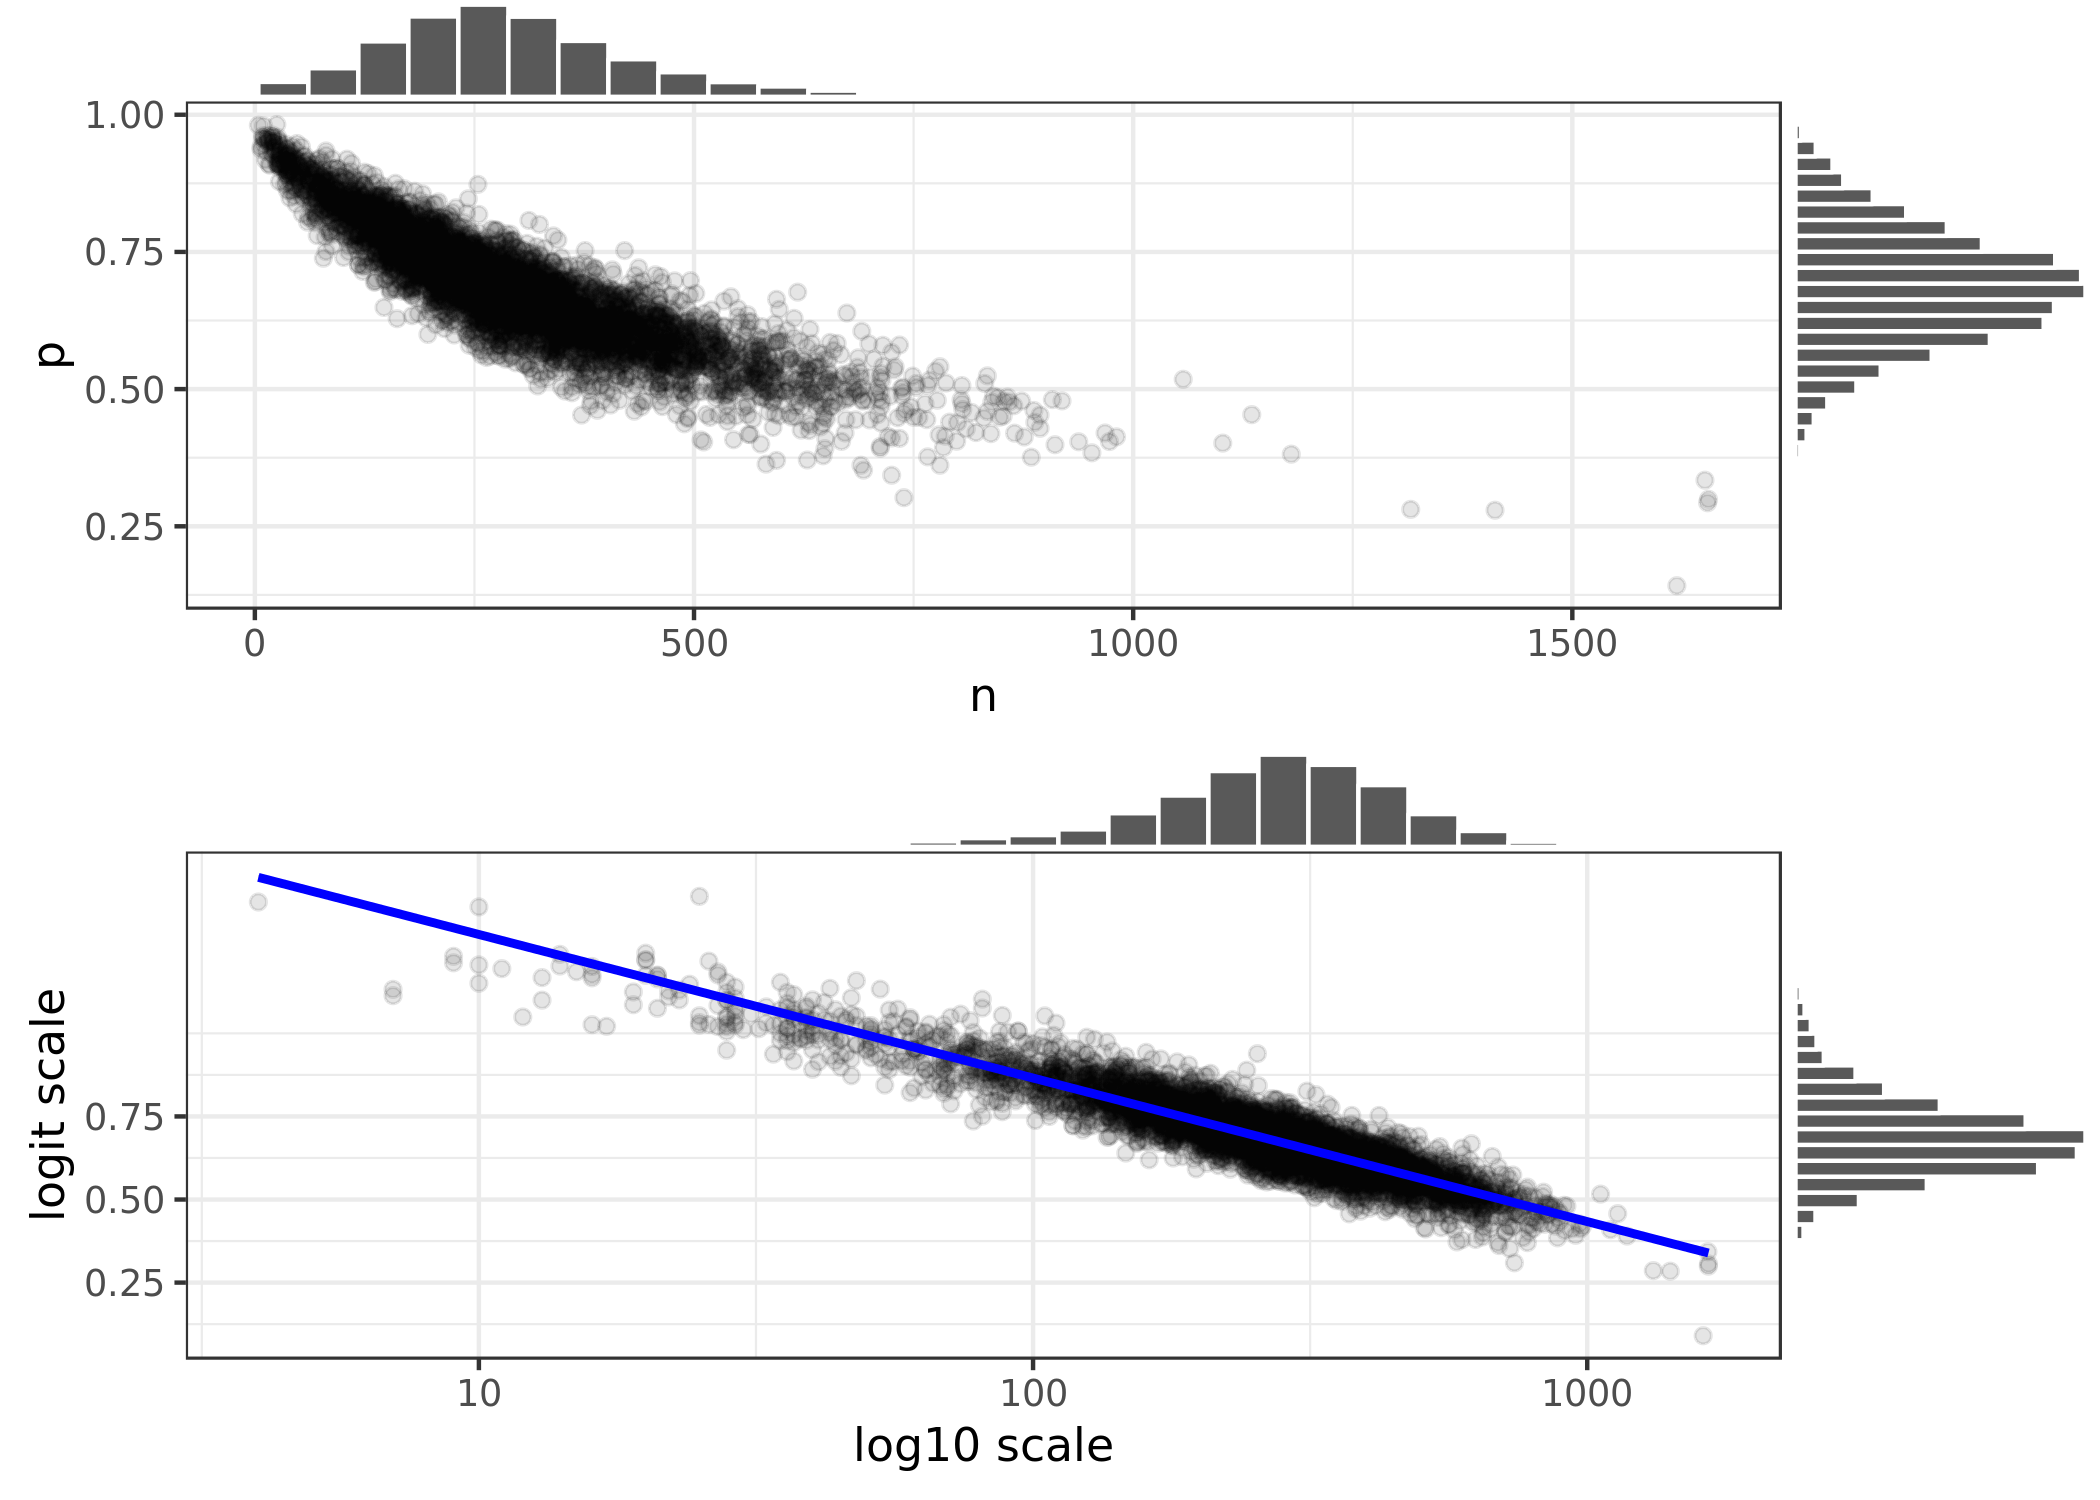
\includegraphics[width=0.9\linewidth]{ambrose_dissertation_files/figure-latex/ghostN-1} 

}

\caption{Ghost probabilities, the sum of document proportion of terms predicted to be present but are actually missing, by document length.}\label{fig:ghostN}
\end{figure}

A document's ghost probability is related to the notion of residuals
that would help assess overall model goodness of fit. A document's per
term residual can be calculated as the observed minus the predicted
document term probability, a document's overall residual the sum of the
squares of the same. These residuals differ from the ghost probabilities
in that they also include the gap in prediction for the terms that do
appear in the original. Either can be used for diagnostic purposes. The
ghost probabilities draw attention to more absurd prediction errors,
while the residuals are more statistically precise. Table
\ref{tab:Kghost} shows the results of two separate linear regressions
which help to rank topics according to each of these goodness of fit
measures while controlling for the powerful effect of document length,
as well as the other topics. In each, the higher the ranking the more
documents within a topic are affected by poor fit. The results are not
consistent between the fit measures. For the ghost probabilities model,
the more a document is composed from topics 8, 2, 3, 5, and 1 the more
likely it is to be predicted to contain terms it does not actually
contain, while documents composed from topics 4, 9 and 6 are more likely
to have their terms accurately predicted. For the residuals model, only
topic 1 is expected to have a poorer fit, while drawing from topics 7,
4, 9, and 8 are all expected to improve document fit. The only topics
for which the direction of effect is in agreement between the models is
topic 1 contributing to bad fit, topics 4 and 9 contributing to good
fit, and topic 10 being neutral.

\begin{table}[!htbp] \centering 
  \caption{Logit of document by topic probability predicting A. logit of ghost probability or B. residual, controlling for log10 of document length} 
  \label{tab:Kghost} 
\begin{tabular}{@{\extracolsep{5pt}} lrrrr} 
\\[-1.8ex]\hline 
\hline \\[-1.8ex] 
Rank & A. Topic & Ghost p Coef. & B. Topic & Residual Coef. \\ 
\hline \\[-1.8ex] 
First & 8 &  0.0498 & 1 &  0.0142 \\ 
Second & 2 &  0.0391 & 10† & -0.0002 \\ 
Third & 3 &  0.0349 & 3† & -0.0018 \\ 
Fourth & 5 &  0.0216 & 6† & -0.0073 \\ 
Fifth & 1 &  0.0176 & 5† & -0.0087 \\ 
Sixth & 7† &  0.0054 & 2† & -0.0091 \\ 
Seventh & 10† & -0.0030 & 8 & -0.0141 \\ 
Eighth & 6 & -0.0177 & 9 & -0.0221 \\ 
Ninth & 9 & -0.0278 & 4 & -0.0245 \\ 
Tenth & 4 & -0.0324 & 7 & -0.0295 \\ 
\hline \\[-1.8ex] 
\multicolumn{5}{l}{† not significant at p < .001} \\ 
\multicolumn{5}{l}{Outcomes normalized to make ceofficents comparable.} \\ 
\end{tabular} 
\end{table}

\hypertarget{junk-terms}{%
\subsubsection{Junk terms}\label{junk-terms}}

Researchers who use topic models usually have a substantive expectation
that there is a transition along the sorted vectors of both document and
term probabilities between true and false classifications. Unfortunately
the model knows no such transition, but interpretations almost always
treat the mathematical feature that all topics are distributions across
all words and all documents are distributions across all topics as a
methodological artifact rather than a desirable result. As we have
mentioned, the satisficing behavior of descending the ranked list until
the researcher feels she has learned something may not be ideal. The
problem is that the ranking used by satisficers may itself be biased due
to the cumulative effect of lower tail probabilities.

A junk term is one that is common but unconcentrated or evenly
classified across all topics. This is the model's way of saying that it
belongs nowhere, which is to say everywhere. If such a term is truly
evenly distributed across topics and documents then the biases would
balance out. However we do not expect language to work this way; what is
more common is that junk terms are parts of suppressed topics, which
would emerge at a higher K, and that these topics are concentrated in
regions of the corpus. If this is true, they will bias upward fitted
topics that are correlated with the suppressed topic. If the suppressed
topic stood in a hierarchical relationship to one topic this would not
be a concern because in effect the child topic could be considered to be
partially constitutive of the parent topic at a lower resolution of K.
However in the expected case of more freely variable topics, unfitted
topics will bias upward the topics with which they are correlated.

Some back of the envelope calculations can illustrate the pitfalls of
junk terms. For argument's sake we can suppose a problematic junk
coefficient to be a function of the length of the global vocabulary
vector such that the bias it might introduce to a topic would appear in
a summation of some large portion of the global vector. Substantively, a
topic ought to be characterized by several dozen or perhaps a few
hundred terms, and because this is a feature of language and cognition
we would expect it to be invariant to the size of the global vocabulary.
However, as the global vocabulary grows the effect of junk terms as a
source of bias increases. In our case we retained 8,390 terms in the
global vocabulary vector. If conservatively we say that a topic is
described by as many as 500 terms, then the unused portion of the global
vector would be 1 - (500 / 8,390) or 94 percent of it.

Now we can consider how large a bias would need to be to be problematic.
A bias of five percent or a proportion of 0.05 could be more than enough
to for instance change a within-document topic ranking. What then is the
sum of the lower tail probabilities (LTP), less than the94th percentile,
of each of the topic by term vectors in our K = 10 model? Table
\ref{tab:k10tail} shows that the lower tail of the distribution ranges
from one quarter to one third of the total topic probability. These are
hardly insignificant portions of the classificatory power of the topics,
but in order for the junk vector to bias a particular document's topic
classification it would need to contain a large number of these terms,
the largest of these lower tail terms being on the order of four
hundredths of a percent. In the especially problematic case it would
also not contain terms in the head of the distribution.

\begin{table}[!htbp] \centering 
  \caption{Sum of topic by term probabilities below 94th percentile.} 
  \label{tab:k10tail} 
\begin{tabular}{@{\extracolsep{5pt}} lrr} 
\\[-1.8ex]\hline 
\hline \\[-1.8ex] 
k & LTP & Max. \\ 
\hline \\[-1.8ex] 
2 & 0.326 & 0.000436 \\ 
3 & 0.317 & 0.000492 \\ 
8 & 0.317 & 0.000434 \\ 
5 & 0.307 & 0.000421 \\ 
7 & 0.277 & 0.000381 \\ 
10 & 0.258 & 0.000383 \\ 
4 & 0.253 & 0.000390 \\ 
1 & 0.252 & 0.000436 \\ 
6 & 0.241 & 0.000398 \\ 
9 & 0.239 & 0.000400 \\ 
\hline \\[-1.8ex] 
\end{tabular} 
\end{table}

Table \ref{tab:worstdoc} illustrates the LTP problem for a document that
we expect to be poorly classified, that is, that has a large portion of
its explained words deriving from a topic's lower tail. The document in
question, a chapter from Mason and McCruden's ``Reading the Epistle to
the Hebrews'', is derived entirely from topic 2, which we may surmise is
about religion.\footnote{www.jstor.org/stable/10.2307/j.ctt1bhkpdr.8}
Here nearly a third of the terms explained by topic two come from the
lower tail. If we assume that these terms are representative of topics
other than religion, then we must conclude that the topic assignment of
this document is biased dramatically upward, that rather than being 100
percent about religion, it is in fact 66 percent about religion, and the
remainder is unexplained. In this case the corrected estimate does not
alter the topic ranking since there is no topic mixture to confuse.

\begin{table}[!htbp] \centering 
  \caption{Lower tail diagnostic for Mason and McCruden's "Reading the Epistle to the Hebrews"} 
  \label{tab:worstdoc} 
\begin{tabular}{@{\extracolsep{5pt}} lrrrrr} 
\\[-1.8ex]\hline 
\hline \\[-1.8ex] 
Topic & Topic Proportion & N Terms Explained & LTP & N from Lower Tail & N from Upper Tail \\ 
\hline \\[-1.8ex] 
2 & 0.999 & 298.597 & 0.325 & 97.130 & 201.466 \\ 
9 & 0.001 &   0.168 & 0.000 &  0.000 &   0.168 \\ 
1 & 0.000 &   0.058 & 0.000 &  0.000 &   0.058 \\ 
10 & 0.000 &   0.052 & 0.000 &  0.000 &   0.052 \\ 
7 & 0.000 &   0.047 & 0.000 &  0.000 &   0.047 \\ 
4 & 0.000 &   0.031 & 0.000 &  0.000 &   0.031 \\ 
8 & 0.000 &   0.023 & 0.000 &  0.000 &   0.023 \\ 
6 & 0.000 &   0.016 & 0.000 &  0.000 &   0.016 \\ 
3 & 0.000 &   0.008 & 0.000 &  0.000 &   0.008 \\ 
5 & 0.000 &   0.001 & 0.000 &  0.000 &   0.001 \\ 
\hline \\[-1.8ex] 
\end{tabular} 
\end{table}

If the terms in the lower tail are on the contrary about religion, then
the document may in fact be correctly classified. Figure
\ref{fig:worstterms} shows the lower tail terms from topic 2 that are
actually present in the text alongside those that are expected to be but
are note present. When sorted by the expected proportion, most of the
terms do not appear to be highly relevant to religion, though some--like
bishop, ritual, homilies, and hell--certainly are. When sorting by those
terms that are actually in the text--such as Levi, eschatological, and
messiah--the religious meaning is much more clear. These results suggest
that the 500 term threshold may be too low for this topic, that it has a
very long list of relevant vocabulary. It is interesting to note that
the term ranking by original document frequency is more suggestive of
religious content, while the predicted frequency, of messiah for
instance, actually dilutes the term ranking. This is an indication of
imperfect fit, as a term like messiah was predicted to be less important
to the text than it actually is.

\begin{figure}

{\centering 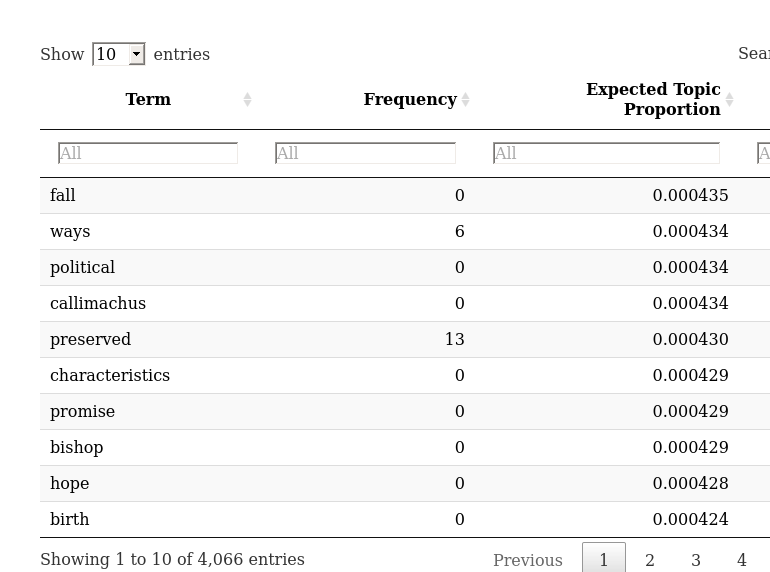
\includegraphics[width=0.9\linewidth]{ambrose_dissertation_files/figure-latex/worstterms-1} 

}

\caption{Terms from Mason and McCruden's "Reading the Epistle to the Hebrews" that are expected to derive from topic 2}\label{fig:worstterms}
\end{figure}

While we have already inspected the summary ranking of topics in terms
of a few measures of goodness of fit, it is helpful to observe the
within topic distributions of LTP, which will make the level of overlap
among topics more clear. First we will inspect the primary topic
classification, as it is common for researchers to reduce the document
by topic probability matrix to the primary classification. Then we will
look at each topic considering all LTPs at once, not just that of the
primary topic.

Figure \ref{fig:worstall} plots the distribution of a document's primary
topic classification, the topic with the highest document by topic
probability for each document, over the document LTP ranking. In other
words, every document is put in a line starting with the highest LTP and
ending with the lowest LTP. The documents are then labeled with their
main topic classification, and a histogram is drawn for each topic
according to counts in bins of 200 along this line. This design mimics
the satisficing behavior of the conventional reader during QVC. Topics
clustered toward the head (left) of the line are composed of poorly fit
documents, and those toward the tail (right) are composed of well fit
documents. The plot shows that some topics are cleanly separated, namely
topics 2, 5, 3, and 8 at the head from topics 9, 6, and 1 at the tail,
with topics 7, 10, and 4 in the middle.

\begin{figure}

{\centering 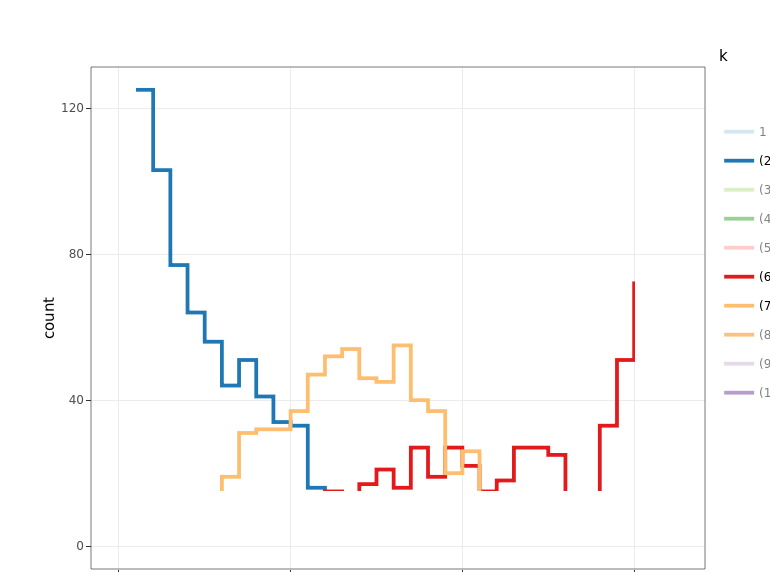
\includegraphics[width=0.9\linewidth]{ambrose_dissertation_files/figure-latex/worstall-1} 

}

\caption{Documents ranked by sum of lower tail probabilities by primary topic classification}\label{fig:worstall}
\end{figure}

For a different view of the problem taking all topic LTPs into account,
Figure \ref{fig:k10headtailp} shows the document distribution by topic
of the LTPs. Rather than looking at only the primary topic, here we
separate each document into its ten topic components, thus each document
is counted ten times, once for each of its topic LTPs. The logarithmic
scale helps us see a fairly even separation, at p = 0.00219, between the
portion of the corpus for which LTPs are and are not a serious
consideration. Below the sag between the two modes the LTPs are
vanishingly small and of no practical concern. Toward the upper mode,
however, we are concerned that the LTPs may be a source of
classification bias. This empirical separation visible on the log scale
is lower than the p = .05 standard that we considered above to be
practically problematic, which covers only the right hand tail of the
upper mode.

When looking at the LTP distribution for all document by topic pairs we
should expect an imbalance in favor of the upper mode, simply because
for every well classified document a few topics will be concentrated in
the head (low LTP) and the rest will be concentrated in the tail (high
LTP). Poorly classified documents will be drawn from the tails of most
topics. Here the lower mode accounts for 52 percent of document by topic
LTPs, so the distribution is more evenly split than we would expect with
strong document classification. This can be visually confirmed by the
nearly balanced shape of the black series, which shows the distribution
of all 10 * 6344 LTPs.

When comparing LTP distribution among individual topics there are clear
differences. Some topics have a much higher proportion of problematic
upper mode LTPs than others. For example, for topic 4 62 percent of
documents are poorly classified, while the same for topic 8 is 34.
Overall, topics 3, 8, and 6 have lower than average LTPs, topics 4, 9,
and 7 have higher than average LTPs, and topics 1 and 10 are close to
the average. Topics 2 and 5 stand out by being more dramatically split
between the two modes, with most of their documents having low LTPs but
a few having some of the highest in the sample.

\begin{figure}

{\centering 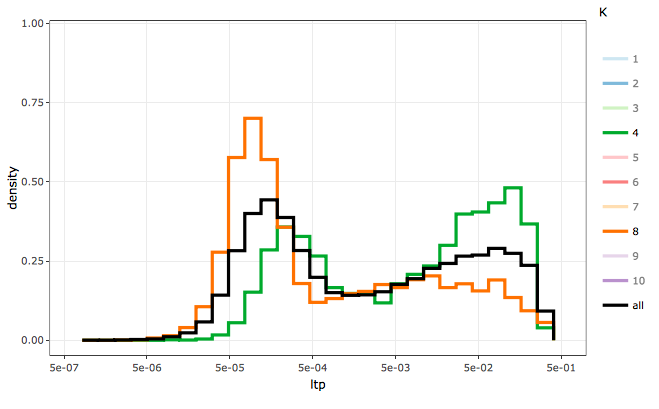
\includegraphics[width=0.9\linewidth]{img/k10headtail} 

}

\caption{Document distribution of sum of lower tail probabilities below 94th percentile by topic, $log_{10}$ scale}\label{fig:k10headtailp}
\end{figure}

Finally, the LTP distributions explored above are based on the arbitrary
cutoff at an index of 500, which we will recall was chosen to divide the
topic by term vectors into true and false segments. To show that topics
actually vary in the length of their relevant term lists, we can hold a
particular LTP proportion constant and see how many terms it takes to
reach that threshold for each topic. Figure \ref{fig:elbow1p} shows the
cumulative proportion of the sorted term list for each topic up to an
LTP cutoff of one third, or an upper head probability of two thirds.
This cutoff is close to the maximum LTP at a constant index of 500, and
indeed we can confirm graphically what was said above that the topic
accounting for the maximum LTP is topic 2. Topics that reach the
threshold early tend to have a more concentrated term vector, that is,
have fewer terms accounting for the same amount of total probability.

Topic 6 reaches the threshold first at an index of 315, which is a
considerably shorter list than 500. Topic 6 also starts with the highest
curve, meaning that it can be summarized by a short list of high
probability terms. Starting high does not necessarily mean a topic will
finish early, as evidenced by topic 10, which starts as high as topic 6
but grows more slowly and finishes late. The reverse is also possible,
as in the case of topic 10 that starts low and finishes early. Topics
can therefore cross each other in the explanatory power of their term
lists. Overall the topics are divided into a faster (topics 6, 9, 4, 10,
1, and 7) and a slower (topics 2, 3, 8, and 5) group.

\begin{figure}

{\centering 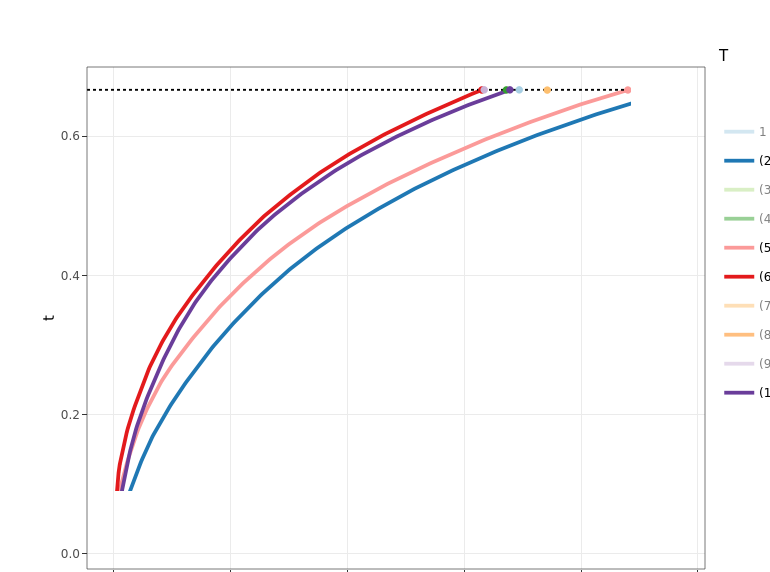
\includegraphics[width=0.9\linewidth]{ambrose_dissertation_files/figure-latex/elbow1p-1} 

}

\caption{Cumulative distribution of within topic term probabilities.}\label{fig:elbow1p}
\end{figure}

While there is no substantive reason to prefer topics with concentrated
term vectors, researchers tend to favor them because they are more
cognitively tractable. It is hard for analysts to make sense of hundreds
of terms; the more a topic can be adequately summarized by a short list
the more easily it is to reify. These diagnostic plots help to identify
the topics which may require additional attention to their lower ranked
terms.

\hypertarget{zero-threshhold}{%
\subsubsection{Zero threshhold}\label{zero-threshhold}}

Whereas junk terms are spread evenly as a function of uncertainty, terms
that are more confidently placed in a few topics are just as confidently
excluded from other topics. It is natural to expect a term that is known
to not belong in a particular topic to be set to zero. However in order
to prevent the estimation of negative probability values, the quantity
estimated is a transformation of the probability that approaches but
cannot meet or pass a zero limit. In the STM model this transformation
is the logarithm which is infinite when transforming a probability of
zero. When these estimates are exponentiated to recover their associated
probability, they will be vanishingly small, and some may even be
returned as zero due to machine limits on the representation of small
numbers. These pseudo zero coefficients are no practical bother as they
are not big enough to sum, even in large numbers, to a significant
probability. A pseudo zero coefficient will be a large negative number
on the logarithm scale, whereas a junk coefficient, a small but
nontrivial probability, will be a smaller negative number.

Zero predictions would make the strict delineation between relevant and
irrelevant terms or documents easy even if it would still be an overly
inclusive standard. It will be helpful to find a natural breakpoint to
establish when model predictions are no longer relevant. It turns out
that an empirical threshold is obvious in the case of documents but not
in the case of terms.

Figure \ref{fig:logit-theta} plots the progression of modal separation
of probabilities at growing levels of K. The modes are most visible in
the log-odds of the probability. When K is less than 5 the distribution
has three modes. In the upper mode are nearly perfectly classified
documents, which suggests counterintuitively that at low Ks it is
actually easier for the model to perfectly separate some documents. This
high mode is mirrored at K=2 by a low mode of the same density, because
for every document probability that is approximately one in one topic
there must be a probability of approximately zero in the other topic. As
K increases the imbalance grows as one implies K - 1 zeroes. But what is
more stark is the vanishing of perfect classifications as K increases,
to the extent that mode in the middle accounting for the bulk of the
distribution is already below .5 even at K = 3. This implies that
mixtures are indeed the normal outcome for document classification when
the model allows it.

\begin{figure}

{\centering 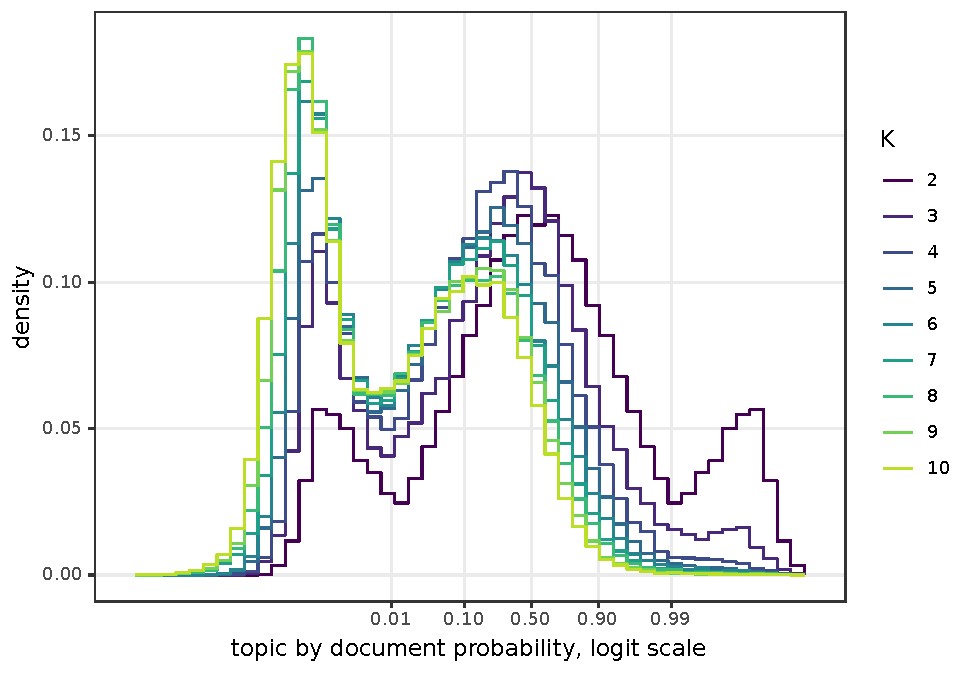
\includegraphics[width=0.9\linewidth]{ambrose_dissertation_files/figure-latex/logit-theta-1} 

}

\caption{As K increases so does separation among junk (lower mode), weak (central mode), and strong (upper mode) topic by document probabilities, logit scale}\label{fig:logit-theta}
\end{figure}

Similarly, Figure \ref{fig:log10-betap} shows the topic probability
distribution but for terms rather than documents. Here there is no neat
separation of modes between zero predictions and substantive ones. At
each K there is a single mode at a very low probability of less than 1
in 10,000. In the figure the body around the mode appears to account for
more of the distribution than is actually the case, as the graph is
truncated at 1e-10. Not shown are the expansive left hand tails of
vanishing probabilities. The portion of the distribution to the left of
an arbitrary point of 1e-6 at the left base of the mode is 10.2 percent
at K = 2 and 47.7 percent at K = 10. Similar to the balancing of ones
and zeroes above, this fattening left tail implies that as K increases
and more terms find a home in a particular topic (as the right tail
thickens) the more those same terms are excluded from the other topics
(the left tail thickens at a faster rate). It is worth noting that from
the model perspective there are many terms that are not in the long left
tail that contribute to document classification for a topic but whose
probabilities are nonetheless so small that researchers are likely to
dismiss them as unimportant. Within the model, a term with a probability
of 1 in 1,000,000 would count as a substantive term belonging to the
body of the distribution.

\begin{figure}

{\centering 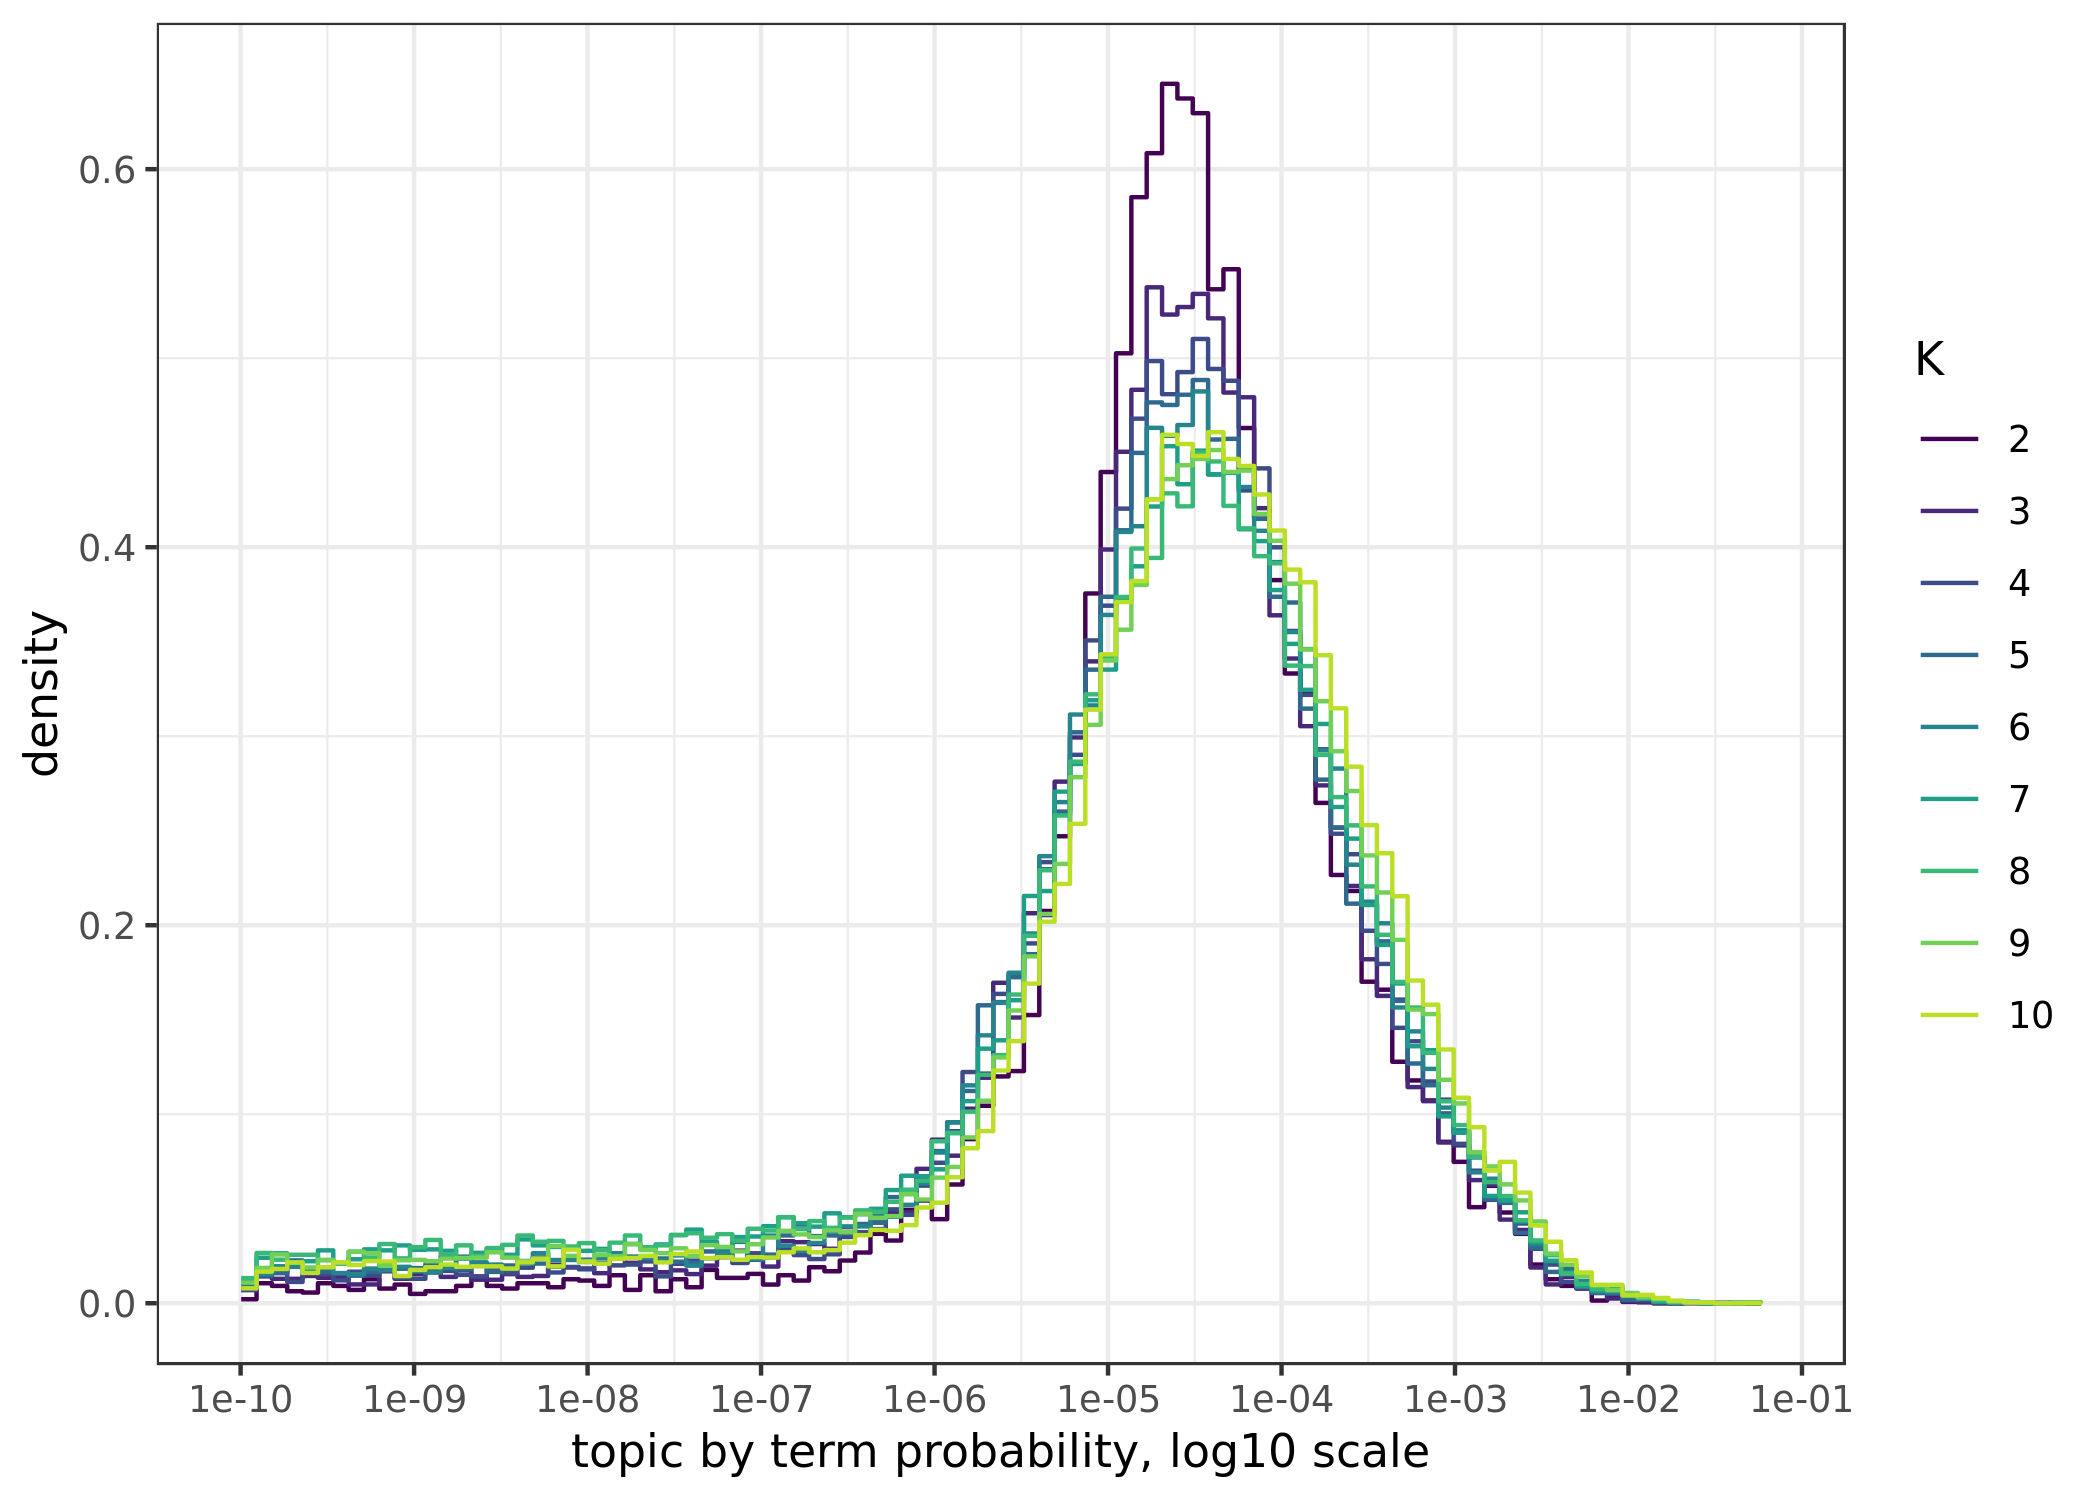
\includegraphics[width=0.9\linewidth]{ambrose_dissertation_files/figure-latex/log10-betap-1} 

}

\caption{As K increases, curve flattens toward more higher and more lower term probabilities, logit scale.}\label{fig:log10-betap}
\end{figure}

We can use the modal separation as a natural break in the log-odds of
the document by topic probabilities to assist us in an enumeration of
the number of documents relevant to each topic. Figure \ref{fig:elbow2}
shows the cumulative distribution of within topic document probabilities
truncated at a threshold of 0.005298, the bottom of the trough between
the middle and lower modes of the K = 10 distribution. Here we see each
distribution rise at a certain rate and flatten off until hitting the
point after which all probabilities are pseudo zero, the point
approximately equal to the topic's share of corpus documents. The linear
trend of the endpoints (dotted line) makes sense given that portions of
documents are counted on the y and whole documents are counted on the x.

Substantively may suspect whether documents near the endpoints are
indeed relevant to the topics, which implies an overcounting of
relevance and a different threshold earlier in the trend perhaps nearer
the elbow of each curve. It may be more useful to compare the relative
landing points as well as the trajectories of the curves. The steeper
the curve at the beginning, the more the topic contains strongly
classified documents. Curves that grow more slowly are more likely to be
in mixtures with other topics, and those that slow rapidly and come to
their endpoint sooner simply represent a smaller segment of the corpus.
Inspecting the first 500 documents shows four separate trajectory
clusters, which do not merely reproduce the ultimate topic sizes. The
low group contains topics 3 and 8. These are the smallest overall topics
by document count, yet inspecting the first 50 documents in each curve
reveals that topic 8 starts with stronger document classifications than
most topics but declines in rank by virtue of representing fewer
documents overall. The next group contains topics 7 and 10, which start
with lower classification strengths than most topics but also maintain
their momentum to eventually land in the middle of the distribution.
Topic 7 especially has a low trajectory but does better at maintaining
it, which may indicate that it is rarely a star but commonly a
supporting actor in document mixtures. The third trajectory
group--topics 6, 5, 2, 4, and 9 by final count--starts in a bundle of
strong classification before diverging rapidly at about index 700 as
they approach their endpoints. Finally on a trend of its own is topic 1,
which sustains strong classifications longer than any other topic.

\begin{figure}

{\centering 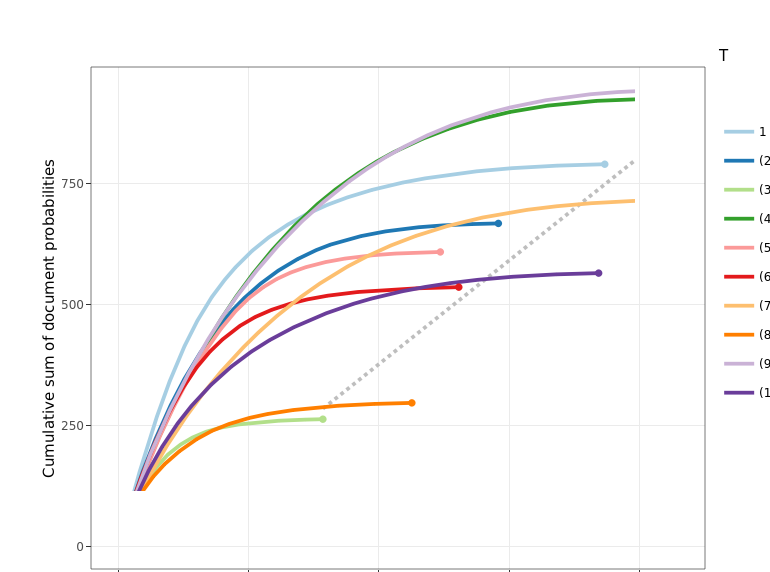
\includegraphics[width=0.9\linewidth]{ambrose_dissertation_files/figure-latex/elbow2-1} 

}

\caption{Cumulative distribution of within topic document probabilities, truncated at junk threshhold. Dashed line is linear fit to endpoints.}\label{fig:elbow2}
\end{figure}

These document trajectories trends provide a view of topic dominance
that is different than the usual ranking of topics by their total corpus
term share. The corpus term share effaces differences in document size
as well as the the fact that rankings change depending on where one
looks along the cumulative distributions. In this model the ranking by
median document probability in the first 300 ordered documents provides
a better view of classification strength among the sets of documents
that researchers are much more likely to focus on during QCV. Table
\ref{tab:topshare} shows that by this document share criterion topics 1,
2, and 6 are much more highly ranked.

\begin{table}[!htbp] \centering 
  \caption{Topic Rankings by Share of Corpus Explained} 
  \label{tab:topshare} 
\begin{tabular}{@{\extracolsep{5pt}} lrrrr} 
\\[-1.8ex]\hline 
\hline \\[-1.8ex] 
Rank & Topic  & Corpus Share & Topic & m300 \\ 
\hline \\[-1.8ex] 
First & 9 & 0.1438 & 1 & 0.914 \\ 
Second & 4 & 0.1409 & 2 & 0.7786 \\ 
Third & 1 & 0.1253 & 6 & 0.7593 \\ 
Fourth & 7 & 0.119 & 9 & 0.7576 \\ 
Fifth & 2 & 0.1057 & 4 & 0.7363 \\ 
Sixth & 5 & 0.0973 & 5 & 0.7279 \\ 
Seventh & 10 & 0.0871 & 10 & 0.638 \\ 
Eighth & 6 & 0.0848 & 7 & 0.5905 \\ 
Ninth & 3 & 0.0495 & 3 & 0.5585 \\ 
Tenth & 8 & 0.0465 & 8 & 0.519 \\ 
\hline \\[-1.8ex] 
\end{tabular} 
\end{table}

\hypertarget{topic-graphs}{%
\subsection{Topic Graphs}\label{topic-graphs}}

Where above we concentrated on individual terms and documents, here we
take several approaches to graphing topics directly.

\begin{itemize}
\tightlist
\item
  A concentration plot organizes topics according to how focused they
  are in particular regions of the document and term vectors.
\item
  A QCV confusion network graphs how easily a naive reader can separate
  topics.
\item
  A topic descent graph contextualizes topic emergence as K increases
  across models.
\end{itemize}

\hypertarget{concentration}{%
\subsubsection{Concentration}\label{concentration}}

Though it was possible to observe concentration during a consideration
of junk vectors, now we will measure concentration directly. Figure
\ref{fig:doc-ginip} shows the topic distribution of the Gini
coefficient, a measure between zero and one where larger values indicate
higher concentration, separately within documents and within terms. The
document distribution has a more normal, the term distribution a more
uniform shape. For documents, a mixture of a handful of topics is the
norm at a median of 0.754. On the right of the distribution a small but
not insubstantial number of documents are highly concentrated, which is
to say classified in only one topic, while on the left is a longer tail
of multivocal, or more likely poorly fit, documents composed of several
topics. For the term distribution there is a wide range of
concentrations of roughly equal size, that may reflect the right-to-left
gradation from monosemy to polysemy and ultimately to topic irrelevance.
The exceptions to uniformity are the discontinuous jump on the right of
anchorlike terms that fall within one topic alone and the long left tail
of guesswork, likely lower frequency terms that the model classified
everywhere and nowhere.

\begin{figure}

{\centering 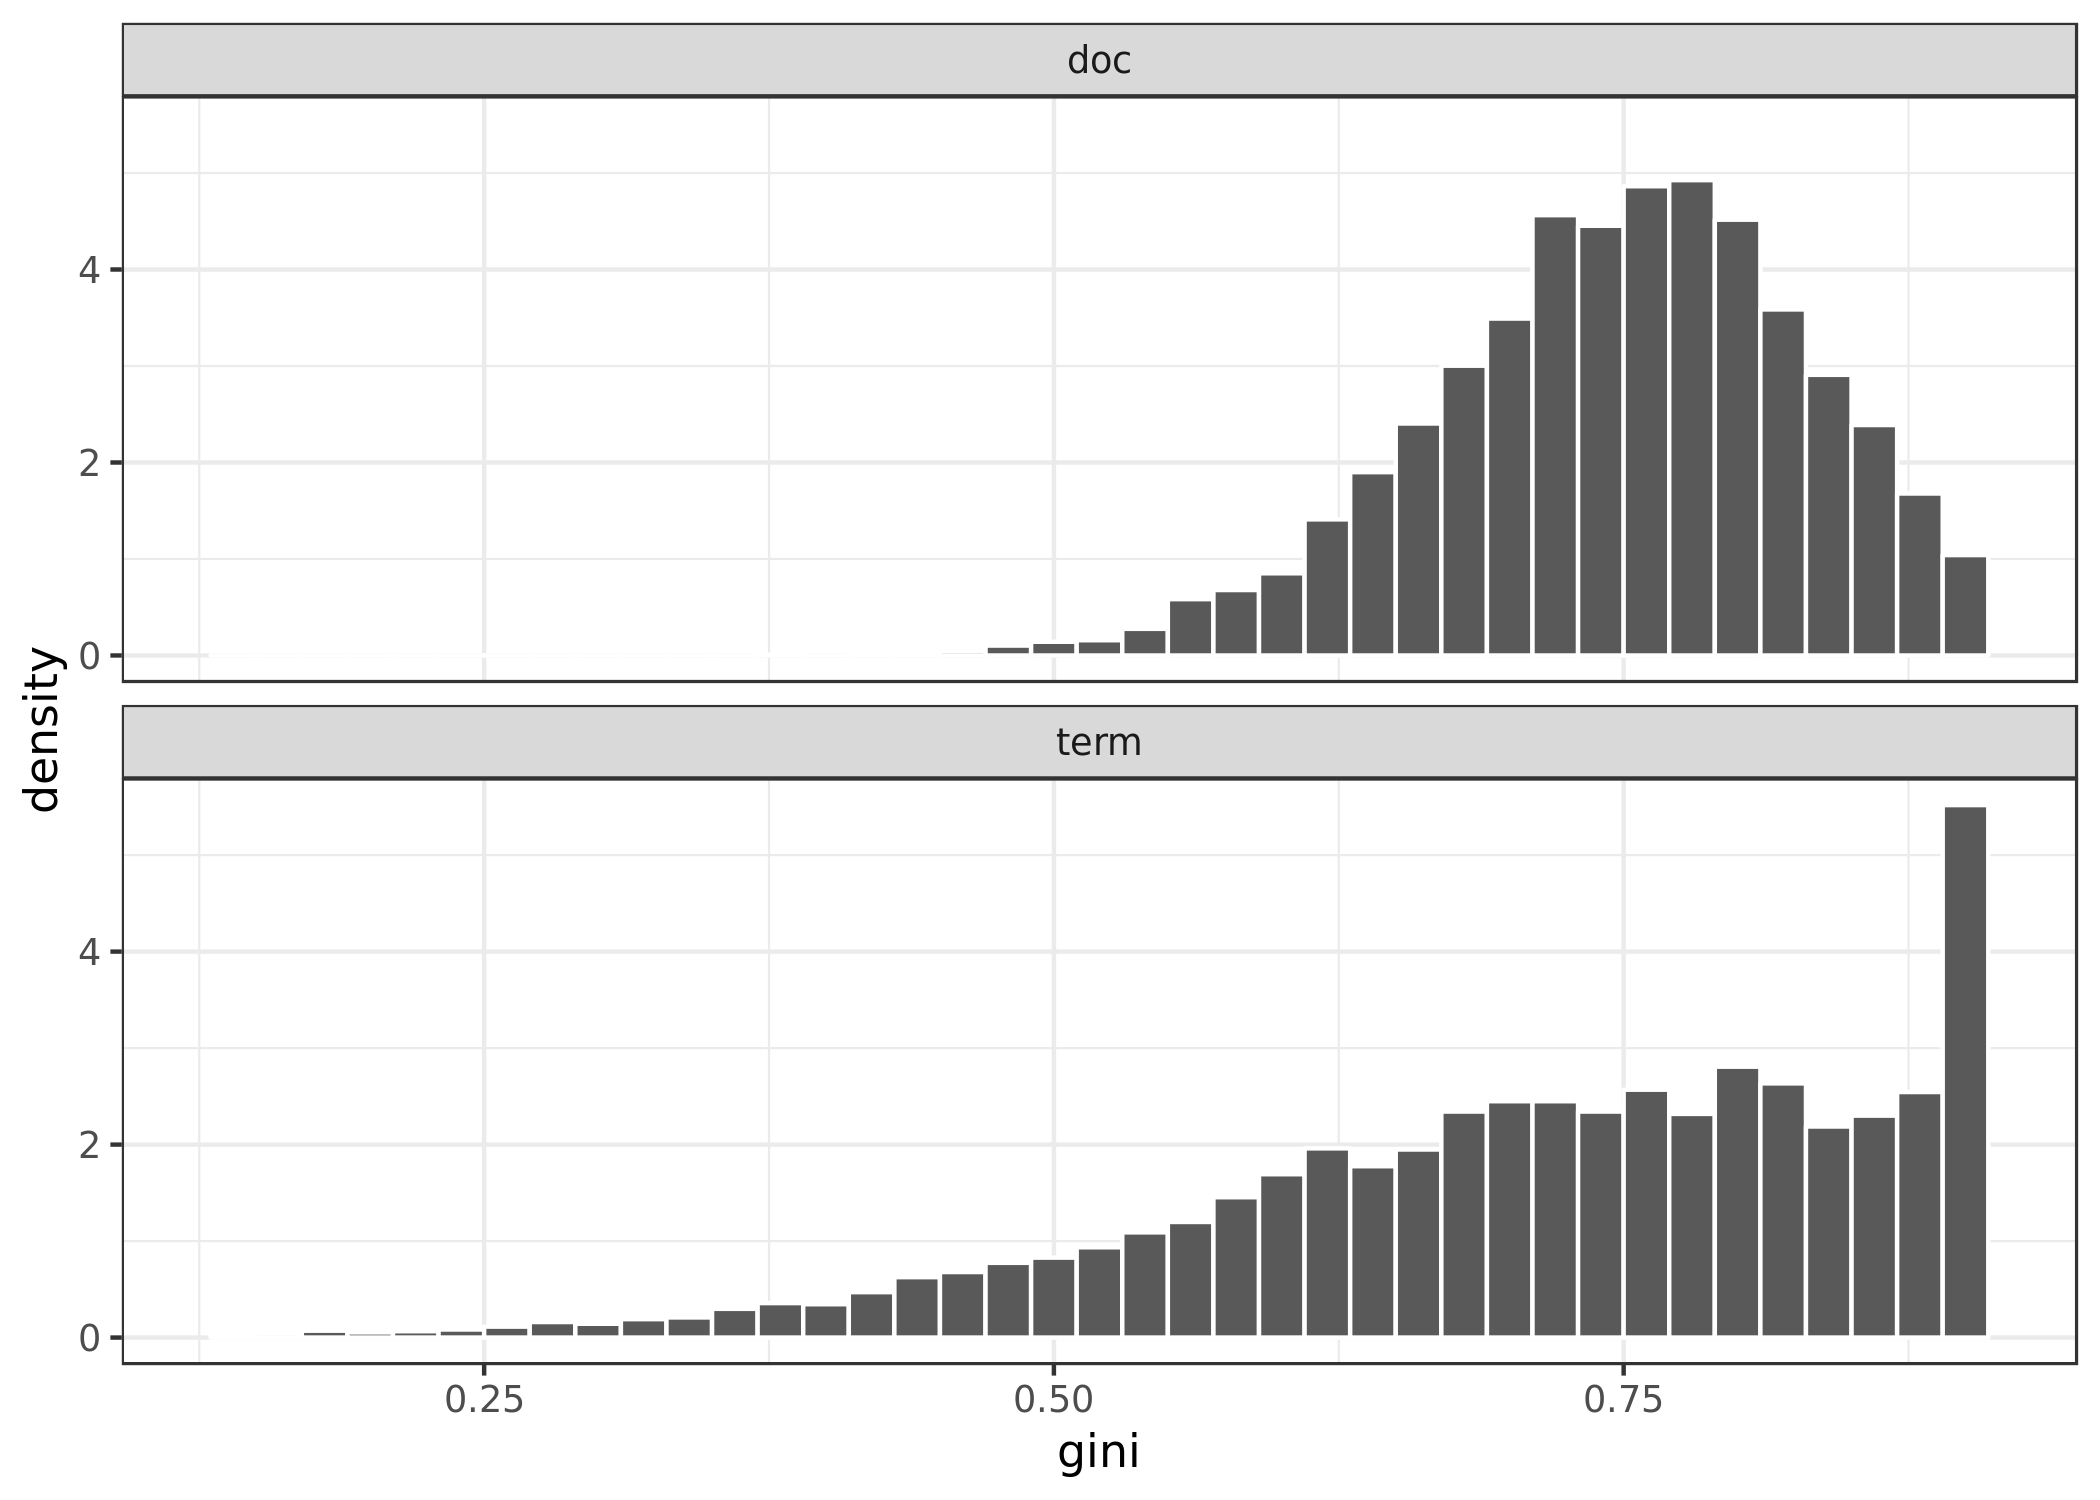
\includegraphics[width=0.9\linewidth]{ambrose_dissertation_files/figure-latex/doc-ginip-1} 

}

\caption{Concentration of topic probabilities within A. documents and B. terms}\label{fig:doc-ginip}
\end{figure}

The concentration idea can be flipped to apply to documents within
topics and terms within topics, and doing so provides useful dimensions
along which to organize topics. The document within topic Gini measures
whether the total document space taken up by the topic is spread evenly
or not, holding constant the size of both documents and topics. The term
within topic Gini on the other hand holds topic size constant but not
term frequency, which is desirable in that minor documents are more
worthy of equal treatment than minor terms. A high term within topic
Gini represents what we noticed above that some topics more than others
can be well described by a relatively short list of important terms.
Figure \ref{fig:top-gini} plots topics along each of these
concentrations. It is divided into four regions split at the median of
each axis. In the green quadrant are topics that are highly concentrated
in both documents and terms, in the red quadrant are topics that are
relatively diffuse on each dimension, and in the yellow are topics that
are concentrated in one but not the other.

\begin{figure}

{\centering 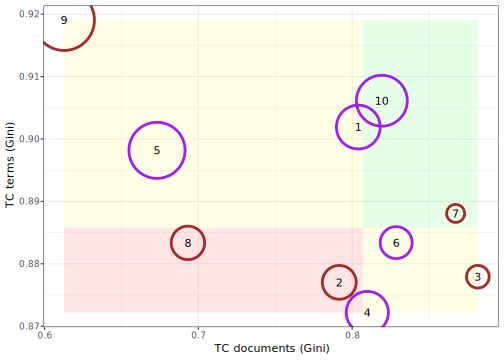
\includegraphics[width=0.9\linewidth]{ambrose_dissertation_files/figure-latex/top-gini-1} 

}

\caption{Topic concentrations (TC) within documents by TC within terms. Diamonds proportional to term frequency explained by each topic}\label{fig:top-gini}
\end{figure}

The concentrations are inversely related such that almost all topics
fall in the yellow quadrants. Indeed only two topics, 6 and 7, fall in
the same half of each distribution. This pattern is partially driven by
size, share of corpus term frequencies, which is proportional to the
area of the black diamonds. Topics composed of fewer terms have less
power to fill up documents and therefore may naturally be more
concentrated in documents. Topic 6 shares the desirable quality of
describing a shorter list of documents and being described by a shorter
list of terms. Topic 7 on the other hand is, notwithstanding being among
the smaller topics, spread out among many documents while having a
diffuse (though not the most diffuse) term list. A group of the smaller
topics (2, 3, and 8) and one larger topic 5 are concentrated in
documents and not terms, while the remaining topics 1, 4, and 10 are
concentrated in terms but not documents. Topic 9 stands out as being
both the most concentrated in terms and least concentrated in documents.
Though it effaces the difference between the yellow quadrants, we
collapse these two dimensions into one by normalizing and averaging each
and assigning an overall concentration rank to each topic.

\hypertarget{blind-qcv}{%
\subsubsection{Blind QCV}\label{blind-qcv}}

Contrary to the conventional approach of inspecting the topic by term
matrix first, I performed a blind QCV sorting test in which I tried to
recover the model classification without prior knowledge of topic
content. This test allows me to interpret topic content from whole texts
rather than from the decomposed topic by term matrix and gives an
opportunity to assess document classification quality prior to
developing a bias about what topic contents mean. It is important to do
this as soon after a model is fit as possible--but after one is
confident that the model won't need to be refit!--so that other work
requiring topic interpretation is not delayed and does not interfere
with validation.

For each topic I created a list with 45 documents to supply five
comparison cases for each of the other nine topics. These lists were the
conventional document by topic rankings sorted in decreasing order of
topic probability. For each of the 45 unordered topic pairs I removed
five articles at random from the document list of each topic and
combined them to create a new randomly shuffled set of ten containing
documents from both topics. The validation task was simply to inspect
each document and attempt to recover the topic groupings, the logic
being that the better the document classification the easier the
sorting. Difficulty was measured by the chi squared probability of the
manual classification against the true classification. An additional
metric of difficulty, the amount of time required to complete the task,
was gathered as well but not used.

Each of the 45 sorting tasks was completed as quickly as possible, which
in practice meant skimming the first page of each document. If this was
enough to suggest the correct groupings the task would be finished. If
the status of some documents was unclear then a closer inspection of the
text would be necessary. Never was a document read closely, so topic
content is still what can be gleaned from a cursory skimming of the
text. Each document appeared only once within a particular topic's list
to avoid the bias of knowing how a document had already been classified
in a previous task. However, because a document could have appeared
twice or more if it was ranked in the top 45 documents of more than one
topic, some documents were seen twice. In these cases the bias would
serve to confuse rather than clarify since the classification would be
different between two instances of the same article.

\begin{figure}

{\centering 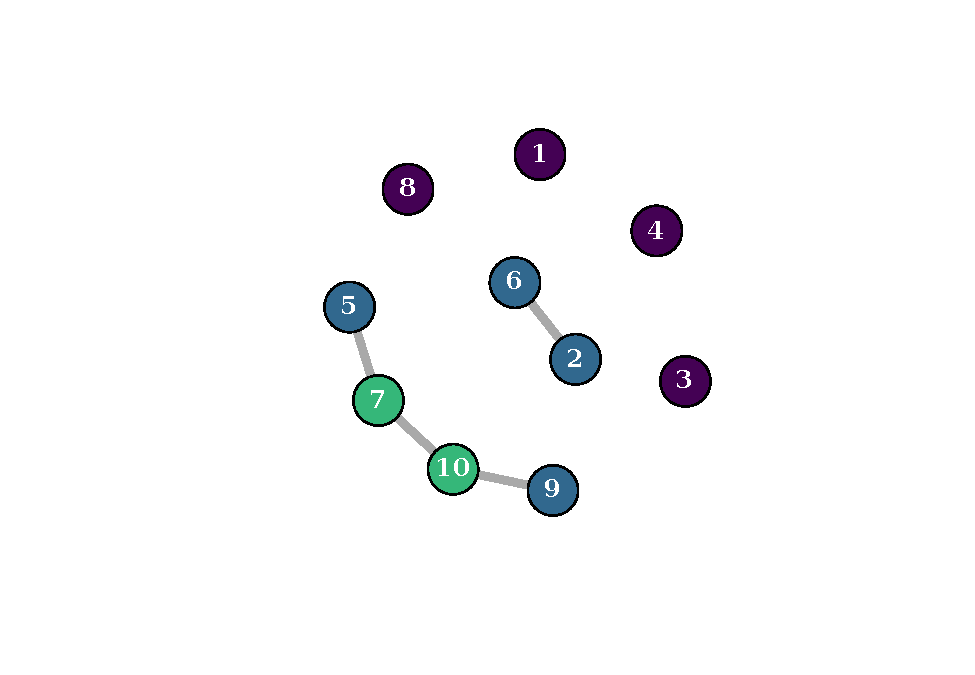
\includegraphics[width=0.9\linewidth]{ambrose_dissertation_files/figure-latex/man-con-1} 

}

\caption{Topic confusion network. Tied topics contained at least two errors in blind manual sorting test. Untied topics were perfectly separated. Colors represent a topic's number of imperfect tests.}\label{fig:man-con}
\end{figure}

Among the 45 different sorting tasks only two outcomes were observed. 41
tasks were performed perfectly (p = 0.0114), while in 4 tasks one error
was made, which is to say two documents were misclassified (p = 0.2059).
Figure \ref{fig:man-con} visualizes the pairwise outcomes as a confusion
network. Topics that are disconnected were sorted perfectly, while
topics that are connected were confused. The graph reveals some
variation in topic confusion, as two were confused twice, four were
confused once, and the remaining four were never confused.

It is not actually clear whether topic confusion is a function of
document misclassification or my lack of familiarity with topic content.
An added benefit of this procedure is that it begins to establish a
theory of each topic by a direct inspection of bellwether texts, and
this growing familiarity decreases the task difficulty over the course
of the testing. In either event the results of this diagnostic provide
an additional basis for understanding interpretive difficulties later.

\hypertarget{topic-descent}{%
\subsubsection{Topic descent}\label{topic-descent}}

All topic models are mixture models in that they treat the observed
document by term frequencies as the outcome of multiple topics mixing
together in different proportions within documents. Whereas the flat
approach treats \emph{documents} as mixtures, a hierarchical topic model
also treats \emph{topics} as mixtures of other topics. Here topics are
mixtures of ancestor nodes in a tree network of topics. A hierarchical
model could, for instance, obviate the procedure of removing common
language syntax words such as articles and prepositions because it could
represent these as a root node of all topics, indicating that all
vocabularies appear in a partial mixture of a language's basic syntax. A
flat model retaining syntax would burden the estimator with learning
that syntax terms should be distributed evenly across all topics. More
substantively, a hierarchical model applied to scholarship may help pick
out fields that have various empirical studies that are nonetheless
united by common theory terms or argumentative style words. Because
substance in its detail can easily swamp framing terminology by sheer
frequency, flat topic model estimators will tend to rends apart fields
where novelty is a virtue and classify them by their minutia rather than
by their themes.

Models and software for hierarchical models have been developed
\citep{Teh2006Hierarchical, Roberts2015pkg}, but they are not yet in
common use by social scientists. Here we use a pseudo hierarchical model
in which we fit separate models at increasing levels of K, and we then
do postestimation to measure the document level overlap among topics
between adjacent levels of K. We refer to this as topic descent, and it
shows how document classification evolves as K increases.

Because a topic descent graph represents relationships only between
K-adjacent models, it is an ensemble of bimodal graphs:

\[G=\{(V_{(2,3)},E_{(2,3)}),(V_{(3,4)},E_{(3,4)}),...(V_{(K-1,K)},E_{(K-1,K)})\}\]

, where each subgraph is a vertex set composed of topics from model
\(k\) and its adjacent model \(k + 1\) from the minimal two topic model
\(V_{(2,3)}\) up to one less than the maximal model \(K\), here
\(V_{(9,10)}\).

\[V_k\in\{(T_{(k,1)},...T_{(k,n)}),(T_{(k+1,1)},...T_{(k+1,n)})\}\] As
bimodal graphs they allow edges only between topics of adjacent models,
that is topic overlaps within models or between models that are two more
more steps apart are not represented. For each pairwise combination of
between model topics, we calculate their overlap as the sum over all
documents of the joint probabilities that a term from a particular
document would come from each topic simultaneously. The document by
topic probabilities are represented by Greek letter theta, \(\theta\).

\[E_{(k,k+1)}={\sum^n_{d=1}\theta_{k,d}*\theta_{k+1,d}}\]

This per pair per document joint probability is the expected portion of
a document that would be simultaneously explained by a topic from model
k and a topic from model k + 1. For example, document one has a
probability of .5 from topic 1 of model k = 2 and a probability of .9
from topic 1 of model k = 3. The expected probability that the models
predict the same portion of document 1 is the joint probability .5 * .9
= .45. It is the chance that the different models make the same
prediction for that document. The sum of this joint probability across
all documents is the total document share that the two topics can be
expected to simultaneously explain if they were statistically
independent. Note that this measure is willfully ignorant of the actual
term overlap between the two topics and is therefore a conservative
estimate. Knowing the term content may allow us to say that in fact all
of the first topic is contained in the the second, in which case the
overlap would be .5 rather than .45.

Figure \ref{fig:sankey} shows the results visualized as a Sankey
diagram. Each stratum contains topics from a single model, and flows
between nodes are the predicted document share overlaps between topics
in adjacent strata. For clarity only the largest (blue) and second
largest (red) flows are visualized, though the graph layout was
calculated using all edges, and the remainder can be inferred from the
edgeless space of each topic. Here we will refer to topics of the final
K = 10 model by number only, like topic 8, but when referring to topics
of ancestor models we will apply the model prefix, e.g.~topic 4 from
model k = 7 will be topic 7k4. By following the main blue flow between
each level it is possible to see topic lineages that extend with
continuity through several K transitions. These lineages have different
depths, ranging from the longest of eight generations leading to topic 2
to the shortest of one generation leading to topic 9.

Four flow patterns are evident. \emph{One to one} (1-1) and \emph{one to
many} (1-m) flows are common at early strata where large topics either
do or do not split when an additional K slot is made available. Note
that each bimodal graph in the ensemble is complete in that each topic
connects to each other topic in the adjacent model. The classification
of a flow between \emph{one} and \emph{many} is a function of the
concentration of flows leading into and out of a topic. \emph{Many}
refers to a set of relatively even flows, whereas \emph{one} refers to a
single dominant flow. For example, in the flows around model k = 3, the
trunk of topic 3k1 splits into two boughs (1-m), whereas the trunk of
topic 3k2 remains intact (1-1). \emph{Many to one} (m-1) flows are
especially interesting, as they identify topics that had previously been
distributed as junk among several topics at the preceding stratum but
that flow together when space is available. These flows form the first
generation of a new lineage, as in topics 5k4, 7k7, and 9k9. Finally
\emph{many to many} flows describe topics that are formed from many
sources but are then immediately disbanded. This is harder to observe
here where most edges are not displayed, but an example is 8k4 which
draws from many topics and is then split in two. The instability of such
topics suggests a lack of validity.\footnote{TODO: Find a concentration
  measure that corrects for small sample bias to help cluster nodes in
  these four categories.}

\begin{figure}

{\centering 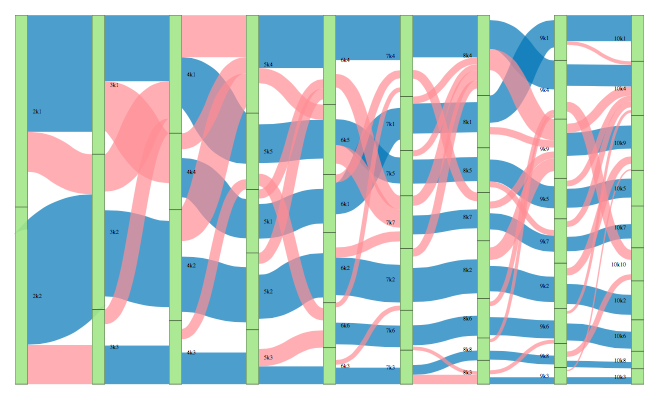
\includegraphics[width=1\linewidth]{img/genre-sankey} 

}

\caption{Sankey diagram of document overlap between topic models of increasing values of K.}\label{fig:sankey}
\end{figure}

The assumption that the depth of a topic's lineage is an indicator of
the strength of its statistical signal implies stability in both the
term and document list for each stratum of the lineage. The truth is
mixed. The longer the lineage the more churn one would expect in term
rankings as its meaning develops toward a more refined vocabulary.
Refinement here means that portions of term frequencies are regrouped
when a k slot becomes available and the smaller portion is pieced out of
the lineage. Figure \ref{fig:lineage} shows the top 40 terms by
probability for the topic 2 lineage. It is clear that there is a gradual
reversal of two main term clusters. Early in the lineage it is driven by
terms relevant to literary studies such as work, text, form, narrative,
book, poem, and author. Certain of these, like literature, narrative,
and history, decline gradually. Others, like text, poem and author,
maintain their status. Unmistakably terms relevant to religion climb in
prominence, with god appropriately rising to take the mantle of topic 2.
Interpreting topic 2 in the context of its lineage suggests that in this
corpus the study of religion is a subfield of literary studies. This has
face validity given the importance of studying texts for both fields. It
would be more difficult to perceive this relationship between literature
and religion taking the conventional approach of using only the lateral
topics within the k = 10 model as context.

\begin{figure}

{\centering 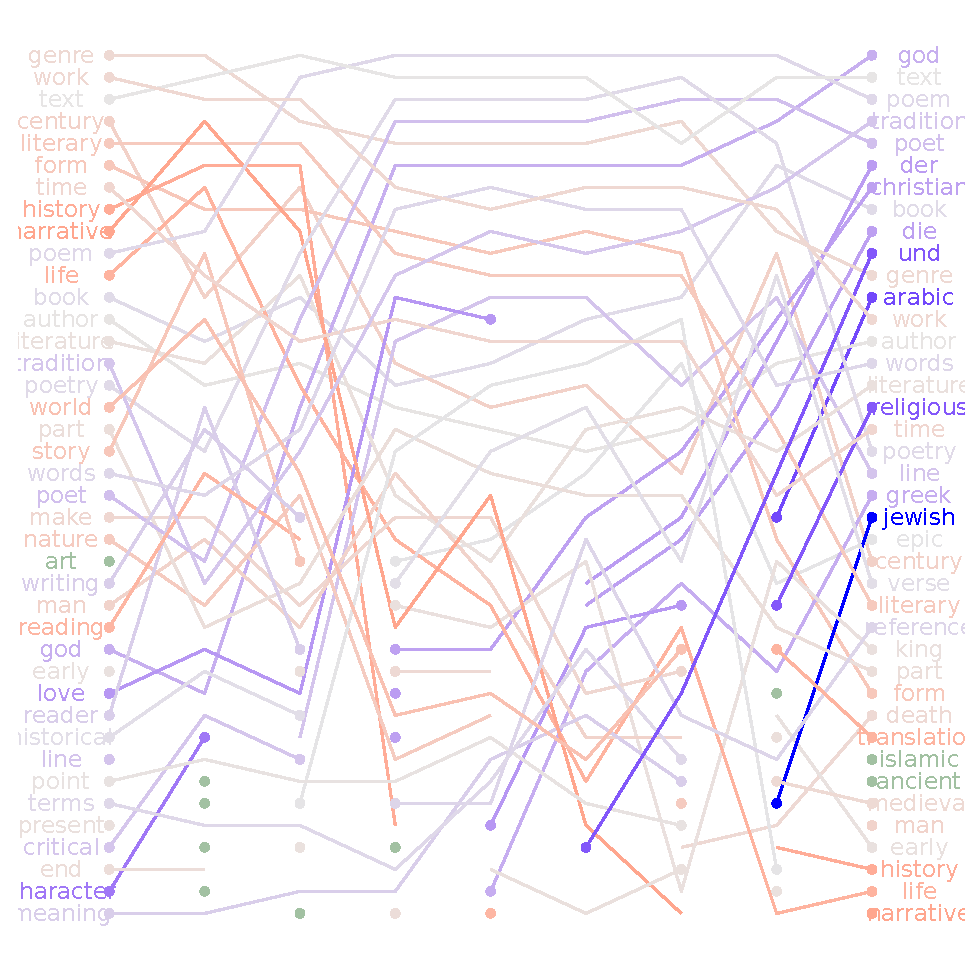
\includegraphics[width=0.9\linewidth]{ambrose_dissertation_files/figure-latex/lineage-1} 

}

\caption{Top 40 term rank changes over topic 2 lineage. Blue are increasing, red decreasing, gray unchanged, and green solitary.}\label{fig:lineage}
\end{figure}

\hypertarget{summary}{%
\subsection{Summary}\label{summary}}

Above we explored ten different features of topics that may affect their
substantive interpretation. We predict that documents from topics with
the following features may be poorly classified, that is, their
substantive content may contradict their topic driven content label. In
general, topics may be considered less valid:

Term level indicators:

\begin{itemize}
\tightlist
\item
  \textbf{Lower tail probabilities}: The higher the topic proportion of
  terms below the topic by term junk threshold.
\item
  \textbf{Term index LTP}: The higher the number of terms required to
  reach the LTP threshold.
\end{itemize}

Document level indicators:

\begin{itemize}
\tightlist
\item
  \textbf{Ghost probabilities}: The higher the average document
  proportion of ghost terms within a topic.
\item
  \textbf{Residuals}: The higher the document differences between the
  predicted and observed term probabilities.
\item
  \textbf{Document Primary Class LTP}: The higher the document
  proportions of terms below the topic by term junk threshold by primary
  topic class.
\item
  \textbf{Document Total Class LTP}: The higher the document proportions
  of terms below the topic by term junk threshold by all topic classes.
\item
  \textbf{Mean bellwether classification strength}: The lower the
  document probability of the first 300 documents of topic.
\end{itemize}

Topic level indicators:

\begin{itemize}
\tightlist
\item
  \textbf{Concentration}: The lower the Gini coefficient topic term and
  document probabilities
\item
  \textbf{QCV Confusion}: The higher the difficulty of blind document
  sorting.
\item
  \textbf{Lineage depth}: The lower the number of ancestors in the topic
  descent lineage.
\end{itemize}

Table \ref{tab:sumrnk} shows the topic rankings for each of these
indicators as well as a summary of all rankings. The highest quality
topic is 6, which is usually in the top three ranks, its exceptions
being higher residuals, a shorter lineage, and some QCV confusion. The
lowest quality topic is 2, its exceptions being the deepest lineage and
strong bellwether classification strength. Topics 6, 9, 1, and 4 may be
separated as a group of higher quality than the rest.

\begin{table}[!htbp] \centering 
  \caption{Summary of Diagnostic Ranks} 
  \label{tab:sumrnk} 
\begin{tabular}{@{\extracolsep{5pt}} lrrrrrrrrrrrrr} 
\\[-1.8ex]\hline 
\hline \\[-1.8ex] 
Rank & ktl & cut & ghst & res & pltp & altp & m300 & gini & conf & ldp & Summary & Rank Mean & Rank Variance \\ 
\hline \\[-1.8ex] 
First & 9 & 6 & 4 & 7 & 9 & 3 & 1 & 6 & 3 & 2 & 6 & 3.5 & 5.4 \\ 
Second & 6 & 9 & 9 & 4 & 6 & 8 & 2 & 3 & 8 & 8 & 9 & 4.2 & 9.1 \\ 
Third & 1 & 4 & 6 & 9 & 1 & 6 & 6 & 1 & 4 & 5 & 1 & 4.5 & 6.1 \\ 
Fourth & 4 & 10 & 10 & 8 & 4 & 2 & 9 & 10 & 1 & 1 & 4 & 4.5 & 7.4 \\ 
Fifth & 10 & 1 & 7 & 2 & 10 & 5 & 4 & 8 & 9 & 4 & 8 & 5.8 & 10.4 \\ 
Sixth & 7 & 7 & 1 & 5 & 7 & 1 & 5 & 9 & 5 & 6 & 3 & 6.3 & 12 \\ 
Seventh & 5 & 5 & 5 & 6 & 8 & 10 & 10 & 5 & 6 & 7 & 5 & 6.3 & 2.5 \\ 
Eighth & 8 & 8 & 3 & 3 & 3 & 7 & 7 & 4 & 2 & 3 & 10 & 6.4 & 5.4 \\ 
Ninth & 3 & 3 & 2 & 10 & 5 & 9 & 3 & 7 & 10 & 9 & 7 & 6.6 & 6.3 \\ 
Tenth & 2 & 2 & 8 & 1 & 2 & 4 & 8 & 2 & 7 & 10 & 2 & 6.9 & 12.8 \\ 
\hline \\[-1.8ex] 
\end{tabular} 
\end{table}

\hypertarget{topic-interpretation}{%
\section{Topic interpretation}\label{topic-interpretation}}

At long last and armored with a diagnostic assessment of the topics, it
is appropriate to interpret the model content of topics. We have three
exhibits to assist us in topic interpretation. First are journal topic
associations. Second are notes taken above during blind QCV of
bellwether texts, which usually amount to gut reactions to the front
matter of articles. Finally we will inspect the topic by term lists
directly. We will initialize each topic interpretation by inspecting
journals and bellwethers, and then we will elaborate the content using
the model lists, being sure to note instances of polysemy.

\hypertarget{journals}{%
\subsection{Journals}\label{journals}}

A good place to begin is to ask whether we have done more than merely
reproduce a categorical scheme we already had access to. If topics are
entirely predicted by journals, then they may not be very valuable as
guides to scholarship, though confirming this would be an argument
against the importance of interdisciplinarity. Figure \ref{fig:jourchi}
shows the relationship between topics and journals when documents are
assigned to their primary topic classification. Each journal is scored
by the standardized \(\chi^2\) residuals from a test of categorical
association between a table of topics by journal document counts. The
standardized residuals can be interpreted as t-scores on a normal
distribution; they represent the distance between observed and predicted
table frequencies in standard errors from what would be expected if the
dimensions were independent. Roughly, scores with a standardized
residual higher than two are worth noting, and the higher the residual
the stronger the association. Rather than sort through all 874 discrete
journals for each topic, I report only the top ten highest residuals.

\begin{figure}

{\centering 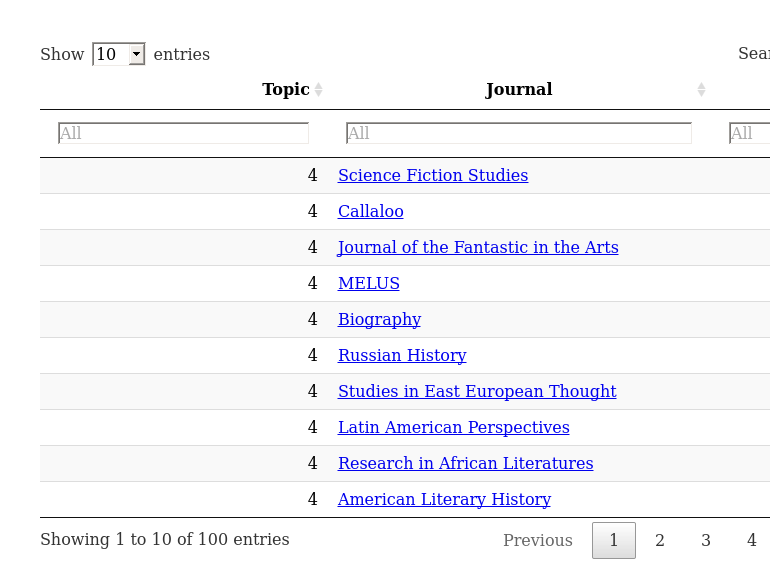
\includegraphics[width=0.9\linewidth]{ambrose_dissertation_files/figure-latex/jourchi-1} 

}

\caption{Journal Topic Associations}\label{fig:jourchi}
\end{figure}

\hypertarget{bellwether-texts}{%
\subsection{Bellwether texts}\label{bellwether-texts}}

Recall that the inspection of bellwethers occurred in the context of a
shuffled list coming from two topics. Notes were taken to record the
rationale that was the basis for splitting the texts into two groups.
Over the course of the 45 separate tasks, themselves shuffled randomly,
the rationales for each topic set in and the sorting task became easier.
Below we characterize each topic based on an inspection of the journals
with which they are associated and the blind QCV notes.

\hypertarget{terms}{%
\subsection{Terms}\label{terms}}




\begin{figure}

{\centering 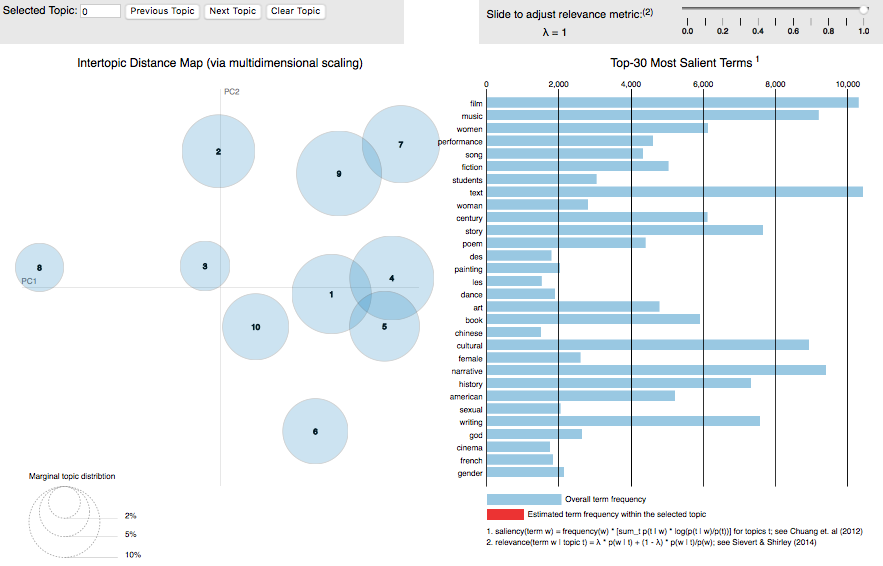
\includegraphics[width=0.9\linewidth]{img/genr-mod-viz} 

}

\caption{Topic Term Explorer, K=10.
\href{ldaviz/viz/index.html}{\emph{Interactive pop-out.}}}\label{fig:genr-mod-viz}
\end{figure}

The topic by term matrix is unwieldy; Figure \ref{fig:genr-mod-viz}
provides a browser generated by the \texttt{LDAvis} package that helps
display topic associations and term lists. In the left panel a
multidimensional scaling technique is used to reduce the term vector two
two dimensions. The area of topic bubbles is proportional to the topic's
share of total corpus frequency, and shorter distances between topics
indicate similarity in term content. In the right panel terms are
displayed as bars with their topic frequency (red) as a share of their
corpus frequency (blue). This list may be sorted by several scoring
techniques that operationalize the notion of exclusivity in different
ways.

First, when no topics are selected, the list is sorted by a score called
saliency. Saliency is a measure of how informative a word is for
guessing the topic from which it comes. Terms that are both very
frequent and very exclusive rise to the top of this list, and indeed the
most salient term ``film'' is very frequent and is an anchor term for
topic 5. Recall that anchor terms are found in one and no other topics.
It is rare to be frequent and an anchor; it is more common that terms
are frequent but salient by virtue of being totally absent from some if
not all other topics. For example, the term ``text'' is common and found
in almost every topic, but is totally absent from topics 5 (film) and 6
(music), which makes sense if text, film, and music are simply different
terms for what is a singular object orientation of each topic. The few
true anchor terms on this list are film (5), les (8), chinese (3),
sexual (7), and cinema (5 again!). Anchor terms for the remaining topics
are too infrequent to show up as globally salient, but they include
literacy (1), biblical (2), utopia (4), musicians (6), hamlet (9), and
painter (10).

Second, when a topic is selected its terms can be ranked by a score
called relevance \citep[66]{Sievert2014LDAvis}. Relevance is a balanced
sum of the overall frequency of a term and its lift, which is its topic
frequency as a proportion of its corpus frequency. The weighting
parameter lambda (\(\lambda\)) sets the balance of the sum. When lambda
is one terms are sorted in the classic order of their topic probability.
When lambda is zero terms are sorted by their exclusivity to the topic
regardless of how infrequent they are (practically, a setting just above
zero allows anchor terms, which all have equal rank and a topic
proportion of one, to be sorted by their frequency). Setting lambda to
zero will put all anchor terms at the top, and empirically it turns out
the anchor list is often quite long. Practically, setting lambda to 0.5
tends to nominate a handful of terms important to the focal topic as
well as others, highlighting cases of polysemy, ambiguity, or true
pantopical relevance.

Recall that goodness of fit during estimation makes reference only to a
topic's ability to explain global corpus frequencies. While relevance
and salience are interesting postestimation techniques, estimation was
not designed to form topics that maximize them. Nonetheless, to the
extent that anchor words are highly relevant, the use of anchor words to
initialize estimation does allow these particularly relevant terms to
impact model results. Though we did not describe the model method of
choosing anchor terms, the ultimate choice remains apparent in the final
model as an artifact. Anchor terms are identifiable as the only terms
for which the fitted log of the probability is -1000, the arbitrary
minimum, for the nine topics for which the term is \emph{not} the
anchor.

\hypertarget{dossiers}{%
\subsection{Dossiers}\label{dossiers}}

Below we assemble the several source of topic interpretation to create a
dossier on each topic, and finally establish for each a theory of topic
meaning. Recall that until this point we have been reticent to describe
such theories for fear of the confirmation bias they will exert on close
readings of texts. These biases are inevitable and the goal is to exert
some control over their formation rather than to presume we may approach
texts from an unbiased vantage point. Thus we expect that in the writing
of dossiers we will at this stage solidify the confirmation bias that
will inform the subsequent ``close, but'' readings of texts. We table
the problem of seriation and proceed in numerical order to aid in later
referencing. Each dossier was written by first completing the initial
characterization from journals, then layering on bellwether
considerations, and finally by inspecting topic term list. For concision
we present all of the results for each topic in one paragraph.

\hypertarget{topic-1-students}{%
\subsubsection{\texorpdfstring{Topic 1,
\emph{students}}{Topic 1, students}}\label{topic-1-students}}

Topic 1 refers to what I above called the ``abstract'' sense of genres
of discourse. The leading journals are different; the first
\emph{Discourse Studies} is general while the second \emph{Research in
the Teaching of English} seems to apply the notion of discourse to the
particular professional domains of education and literacy. During QCV
the importance of discourse was never noticed, and it was almost
entirely taken to be about teaching and pedagogy especially with respect
to writing. A few articles dealt with technical writing in business
rather than in education contexts. From the term lists the model anchor
``remake'' is not expected, and in fact we might have expected it to
occur in topic 5. The bulk of the terms are related to education. Not
only ``discourse'' but ``writing'', ``reading'', and ``text'' share
considerable overlap with other topics, and may help place topic 1 in a
central location on the topic map.

\begin{table}[!htbp] \centering 
  \caption{Topic 1 Terms} 
  \label{tab:t1d} 
\begin{tabular}{@{\extracolsep{5pt}} lr} 
\\[-1.8ex]\hline 
\hline \\[-1.8ex] 
lambda & Terms \\ 
\hline \\[-1.8ex] 
 & model anchor: remake \\ 
0.01 & literacy, students, classroom, data, grade, curriculum, learners, textbooks, pedagogy, courses \\ 
0.5 & students, research, writing, study, teachers, genre, language, discourse, learning, information \\ 
1 & genre, writing, students, text, study, language, research, discourse, social, reading \\ 
\hline \\[-1.8ex] 
\end{tabular} 
\end{table}

\hypertarget{topic-2-god}{%
\subsubsection{\texorpdfstring{Topic 2,
\emph{god}}{Topic 2, god}}\label{topic-2-god}}

Topic 2, which above we interpreted as religious studies, is here led by
the journal \emph{Quaderni di Studi Arabi}, which is dedicated to the
culture and history of Arab civilization. While that scope may include
religion we would expect it to extend far beyond it. While there are
certainly more explicitly religious journals among the list, there are
also journals dedicated to antiquity. This helps broaden our
understanding of the topic, which is more about the history of Abrahamic
civilization than about religion narrowly. We should also resist a
western centric notion of religion, as we are bound to discover
important religious themes in topic 3. During QCV this was often labeled
as ``biblical'' with occasional reference to Islam or the Quran or
Hellenism. Indeed the most relevant term ``ibn'' means ``son of'' in
Arabic names. The model anchor ``Twain'' seems fairly oblique to the
topic although Mark Twain may have spoke frequently of god. The term
lists remind us that underlying biases in publishing, here the over
representation of Christian topics, can be reproduced with a naive focus
on high frequency terms.

\begin{table}[!htbp] \centering 
  \caption{Topic 2 Terms} 
  \label{tab:t2d} 
\begin{tabular}{@{\extracolsep{5pt}} lr} 
\\[-1.8ex]\hline 
\hline \\[-1.8ex] 
lambda & Terms \\ 
\hline \\[-1.8ex] 
 & model anchor: twain \\ 
0.01 & ibn, biblical, jesus, prophet, arabic, hebrew, testament, ovid, virgil, persian \\ 
0.5 & god, christian, der, und, arabic, jewish, die, greek, islamic, ibn \\ 
1 & god, text, poem, tradition, poet, der, christian, book, die, und \\ 
\hline \\[-1.8ex] 
\end{tabular} 
\end{table}

\hypertarget{topic-3-chinese}{%
\subsubsection{\texorpdfstring{Topic 3,
\emph{chinese}}{Topic 3, chinese}}\label{topic-3-chinese}}

Topic 3 includes several pan Asian studies journals as well as journals
focusing on Japan and China. Like topic 8 the signal in likely due to
language and cultural content and perhaps more simply geographical
terminology like state names. Unlike topic 8 they were not drawn into
the sample because of a coincidental meanings of ``genre'' in French.
During QCV a specifically historical thrust was apparent especially with
reference to Chinese imperial dynasties. Interestingly Hittite
civilization appeared more than once, which is geographically closer to
the content of topic 2 but nonetheless categorized separately. Several
references were made to the Song dynasty, which poses a true polysemy
and disambiguation challenge with respect to topic 6.\footnote{Only
  challenging due to the preprocessing decision to convert all terms to
  lower case. Had ``Song'' and ``song'' been left separate,
  disambiguation would not have been a problem. The model estimates that
  14 percent of instances of song are from topic 3 and 82 percent are
  from topic 6.} The terms contain many more proper nouns, place and
person names, than other topics, and raise the importance of Japanese
and Korean topics that were not as apparent in the bellwethers.

\begin{table}[!htbp] \centering 
  \caption{Topic 3 Terms} 
  \label{tab:t3d} 
\begin{tabular}{@{\extracolsep{5pt}} lr} 
\\[-1.8ex]\hline 
\hline \\[-1.8ex] 
lambda & Terms \\ 
\hline \\[-1.8ex] 
 & model anchor: shuo \\ 
0.01 & chinese, china, shi, korean, wang, buddhist, zhang, tokyo, liu, shu \\ 
0.5 & chinese, japanese, china, japan, korean, shi, hong, wang, liu, han \\ 
1 & chinese, text, japanese, china, song, line, time, japan, century, work \\ 
\hline \\[-1.8ex] 
\end{tabular} 
\end{table}

\hypertarget{topic-4-fiction}{%
\subsubsection{\texorpdfstring{Topic 4,
\emph{fiction}}{Topic 4, fiction}}\label{topic-4-fiction}}

Topic 4 is almost exclusively concentrated in the journal \emph{Science
Fiction Studies}, with a smattering of weaker associations across a
diverse set of journals. This suggests a fairly narrow focus, not even
of fiction but a subgenre of it. During QCV the topic was difficult to
disentangle, though ultimately it was not confused with any other topic.
It was often noted to be fiction or science fiction, but as often it
included the analysis of cultures of utopianism or futurism, often
applied in nonfiction settings, for instance, to study historical
narratives in support of political racism and in various locations like
the American west, the USSR, and post colonial Africa. Inspecting the
term lists seems to efface the prominence of science fiction in favor of
a political and historical terminology, though the model choice of
Asimov for an anchor is a helpful reminder of the journal origin of the
topic. The mixing of fiction and nonfiction topics may be a symptom of
poor fit, or there may be a real elective affinity intersecting on
utopianism.

\begin{table}[!htbp] \centering 
  \caption{Topic 4 Terms} 
  \label{tab:t4d} 
\begin{tabular}{@{\extracolsep{5pt}} lr} 
\\[-1.8ex]\hline 
\hline \\[-1.8ex] 
lambda & Terms \\ 
\hline \\[-1.8ex] 
 & model anchor: asimov \\ 
0.01 & utopia, utopian, postcolonial, slavery, douglass, dystopian, suvin, soviet, stalin, genocide \\ 
0.5 & fiction, political, science, history, american, cultural, narrative, story, world, national \\ 
1 & fiction, political, narrative, cultural, history, story, world, american, social, science \\ 
\hline \\[-1.8ex] 
\end{tabular} 
\end{table}

\hypertarget{topic-5-film}{%
\subsubsection{\texorpdfstring{Topic 5,
\emph{film}}{Topic 5, film}}\label{topic-5-film}}

Topic 5 is very well represented among a variety of journals dedicated
to film and cinema. We wonder if the quantity of journals is reflective
of industry support. Mixed with film articles were several related to
television and one related to video games, perhaps sharing terms in
common to the description of U.S. industrial entertainment media. The
horror genre appeared to be over represented. We may speculate that
subtopics with more exclusive vocabulary, even if they are a minority of
cases, may come to be more representative of a topic than one would
expect. Indeed the term lists reveal ``Dracula'' to be the model anchor
and ``zombie'' and ``horror'' to be highly relevant, whereas ``noir'' is
the only other subgenre term showing up in the top ten lists. While it
is possible that horror is actually over represented in film
scholarship, the model behavior suggests that it merely has a more
distinctive vocabulary. Topic 5 was confused once with 7, perhaps due to
the importance of storytelling to each.

\begin{table}[!htbp] \centering 
  \caption{Topic 5 Terms} 
  \label{tab:t5d} 
\begin{tabular}{@{\extracolsep{5pt}} lr} 
\\[-1.8ex]\hline 
\hline \\[-1.8ex] 
lambda & Terms \\ 
\hline \\[-1.8ex] 
 & model anchor: dracula \\ 
0.01 & film, cinema, movie, hollywood, shot, cinematic, lms, filmmakers, camera, zombie \\ 
0.5 & film, cinema, movie, television, hollywood, game, horror, shot, noir, director \\ 
1 & film, genre, cinema, movie, american, audience, character, time, show, production \\ 
\hline \\[-1.8ex] 
\end{tabular} 
\end{table}

\hypertarget{topic-6-music}{%
\subsubsection{\texorpdfstring{Topic 6,
\emph{music}}{Topic 6, music}}\label{topic-6-music}}

Topic 6 has several strong journals led by \emph{Popular Music}, and
interestingly \emph{Asian Theatre Journal}. Farther down the list are
discipline specific journals. The music topic was obvious and noted to
be sorted with particular ease during QCV but was actually confused once
with topic 2. The model anchor ``jin'' is probably a reference to the
Jin dynasty in China, which indicates a curious segregation of the
historical relevance of music in a presumably theater context from the
rest of topic 3, where the model assumes that the term Jin is
\emph{never} discussed. Similarly, it is telling that the term
``Indonesian'' can be understood by its placement as an exclusive term
in a music category to never be relevant to another topic. We might
expect historical geographies to be relevant in all of their cultural
dimensions, but at least with reference to the term genre there is
considerable topic segregation.

\begin{table}[!htbp] \centering 
  \caption{Topic 6 Terms} 
  \label{tab:t6d} 
\begin{tabular}{@{\extracolsep{5pt}} lr} 
\\[-1.8ex]\hline 
\hline \\[-1.8ex] 
lambda & Terms \\ 
\hline \\[-1.8ex] 
 & model anchor: jin \\ 
0.01 & music, dance, musicians, jazz, singer, rap, drum, hop, hip, indonesian \\ 
0.5 & music, performance, song, dance, singing, musicians, singer, folk, record, band \\ 
1 & music, performance, song, cultural, dance, popular, genre, play, tradition, record \\ 
\hline \\[-1.8ex] 
\end{tabular} 
\end{table}

\hypertarget{topic-7-women}{%
\subsubsection{\texorpdfstring{Topic 7,
\emph{women}}{Topic 7, women}}\label{topic-7-women}}

Topic 7, like 4, is concentrated in one journal, \emph{Marvels and
Tales} which is about folklore, yet the second journal \emph{Culture,
Health \& Sexuality} could not seem more different. Two other journals
relate to women's studies, and several other journals relate
specifically to British folklore. During QCV this topic was
misunderstood as two different topics, one about folklore and one about
gender and sexuality often with reference to youth and family. This may
help explain why topic 7 was confused twice, once with 5 and once with
10. It is possible that the importance of family and gender in folk
tales, for instance Arthurian tales of chivalry, allows folklore to be
merged with modern gender studies. The model anchor ``Archie'' likely
relates to problematic gender assumptions in the comic book series. The
term lists otherwise describe a topic that is unequivocally about gender
and sexuality, with queer topics showing up as highly relevant. Only one
hint of folklore, Gawain, is observable in the top ten lists. Farther
down the list especially at lambda = 0.5 are terms specific to family
relationships, ``husband'' for instance being an anchor word.

\begin{table}[!htbp] \centering 
  \caption{Topic 7 Terms} 
  \label{tab:t7d} 
\begin{tabular}{@{\extracolsep{5pt}} lr} 
\\[-1.8ex]\hline 
\hline \\[-1.8ex] 
lambda & Terms \\ 
\hline \\[-1.8ex] 
 & model anchor: archie \\ 
0.01 & sexual, feminine, heroine, husband, queer, lesbian, homosexuality, heterosexual, maternal, gawain \\ 
0.5 & women, woman, female, sexual, gender, male, love, mother, men, tale \\ 
1 & women, story, woman, narrative, female, love, men, sexual, gender, male \\ 
\hline \\[-1.8ex] 
\end{tabular} 
\end{table}

\hypertarget{topic-8-les}{%
\subsubsection{\texorpdfstring{Topic 8,
\emph{les}}{Topic 8, les}}\label{topic-8-les}}

Topic 8 is seemingly related to French and music studies but is led by
the biology journal \emph{Crustaceana} and includes \emph{Botanical
Review}. This collection is likely united by the appearance of many
French language terms, caught in the initial sample definition of the
common French term ``genre'', which after all is a French loanword
translating to ``kind'' but in the native tongue referring to much more
than culture. Indeed genre also has the more special meaning ``genus''
which explains the appearance of life science journals. These errors
should be removed from the sample but they provide an instructive
challenge, or perhaps an easy win, for the topic model estimator.
Unfortunately removing texts by the topic score may actually eliminate
substantive texts that happen to deal with French language content but
are relevant to genre studies, so removal by journal is more
appropriate. During QCV several articles related to orchestral music,
one of which was in Italian not French, and Gregorian chants appeared.
It was noted that English language articles had the term genre included
in a French translation of their abstracts, an in this case nuisance
feature of the JSTOR search not disabled by a specific filtering by
language. The term list is populated with not only French but also
Spanish and Italian stopwords. Topic 8 is so different that it forms its
own axis in the scaled topic map.

\begin{table}[!htbp] \centering 
  \caption{Topic 8 Terms} 
  \label{tab:t8d} 
\begin{tabular}{@{\extracolsep{5pt}} lr} 
\\[-1.8ex]\hline 
\hline \\[-1.8ex] 
lambda & Terms \\ 
\hline \\[-1.8ex] 
 & model anchor: epiphany \\ 
0.01 & les, del, qui, une, pour, una, motet, madrid, chanson, tout \\ 
0.5 & les, des, del, paris, french, est, spanish, qui, une, france \\ 
1 & les, des, french, paris, spanish, del, est, text, work, century \\ 
\hline \\[-1.8ex] 
\end{tabular} 
\end{table}

\hypertarget{topic-9-genre}{%
\subsubsection{\texorpdfstring{Topic 9,
\emph{genre}}{Topic 9, genre}}\label{topic-9-genre}}

Topic 9 has one leading journal (\emph{New Literary History}) like 7 and
4, but there is a clear ``language and literature'' trend among even the
more weakly associated journals. It is interesting that the second
journal \emph{L'Esprit Créateur} is a French language journal; we may
anticipate some overlap with the French language topic 8 that may
suppress its prominence here. Also our limited glimpse at topic 2 to
illustrate topic descent above revealed the importance of poetry, and
topic 9 includes \emph{Victorian Poetry}. If the term poem is indeed
important to topic 9, then it is a caveat against interpreting a term
important across multiple topics as exhibiting polysemy, since here it
would clearly have the same meaning just in different substantive
contexts. During QCV it was sometimes hard to sort, and sometimes
treated as separate literary theory and philosophy topics. It is
possible that elements of style, such as a stilted or abstract diction,
cause these areas to merge. Indeed the likely derogatory model anchor
``simplified'' may reveal that high minded bickering is characteristic
of style more than content! As with topic 7, the error of positing two
topics to describe one leads to a higher confusion rate with other
topics. More than any other topic the relevant terms are the names of
important figures usually real and sometimes imagined. The frequent
terms suggest literature, and the relevant terms suggest philosophy.
Either the two fields are erroneously merged or literary theory merely
draws heavily on philosophy.

\begin{table}[!htbp] \centering 
  \caption{Topic 9 Terms} 
  \label{tab:t9d} 
\begin{tabular}{@{\extracolsep{5pt}} lr} 
\\[-1.8ex]\hline 
\hline \\[-1.8ex] 
lambda & Terms \\ 
\hline \\[-1.8ex] 
 & model anchor: simplified \\ 
0.01 & hamlet, hegel, yeats, derrida, schlegel, pushkin, dostoevsky, nietzsche, kant, sonata \\ 
0.5 & genre, poem, poetry, form, literary, nature, theory, poetic, critical, tragedy \\ 
1 & genre, form, work, literary, poem, poetry, nature, text, critical, narrative \\ 
\hline \\[-1.8ex] 
\end{tabular} 
\end{table}

\hypertarget{topic-10-painting}{%
\subsubsection{\texorpdfstring{Topic 10,
\emph{painting}}{Topic 10, painting}}\label{topic-10-painting}}

Topic 10 is distributed among several journals about art, including a
couple of Renaissance studies journals. During QCV this was easy to
separate and was labeled painting, as in ``Dutch genre painting''. Topic
10 was confused twice, once with 7 and once with 9. The term lists
suggest painting but also book publishing and place names specific to
the British isles, whereas bellwethers much more strongly evoked Belgium
and the Netherlands. The confusion stems from the reader seeing two
topics, the British novel on one hand and painting on the other, where
in the model they are collapsed, perhaps due to the prominence of London
in both art dealing and book publishing.

\begin{table}[!htbp] \centering 
  \caption{Topic 10 Terms} 
  \label{tab:t10d} 
\begin{tabular}{@{\extracolsep{5pt}} lr} 
\\[-1.8ex]\hline 
\hline \\[-1.8ex] 
lambda & Terms \\ 
\hline \\[-1.8ex] 
 & model anchor: rosenberg \\ 
0.01 & painting, irish, painter, dickens, wilkie, scottish, scotland, portraiture, canvas, gaelic \\ 
0.5 & painting, letter, art, century, book, published, print, london, artists, england \\ 
1 & century, book, work, art, painting, letter, history, published, london, english \\ 
\hline \\[-1.8ex] 
\end{tabular} 
\end{table}

\hypertarget{topic-clusters}{%
\section{Topic clusters}\label{topic-clusters}}

Having posited a nominal theory of each topic by inspection of journals,
bellwether texts, and the topic by term matrix, we have not yet
established what documents are about. Because the topic model is a
mixture model we have at best understood what the potential for document
composition is, not what their compositions actually are. Understanding
the patterns of topic mixtures, or topic clustering, within documents is
the last necessary analysis at a global level before proceeding with a
stratification of the corpus for purposes of reading. Here we take two
approaches to document clustering, first by hierarchical clustering of
the distances between documents calculated directly from the document by
topic matrix, and second by network community detection.

Agglomerative hierarchical clustering works by first calculating the
euclidean distance between points in an n-dimensional space, either as
documents in a vector space of topics or as topics in a vector space of
documents. The data are naturally scaled to sum to one in the document
dimension; before calculating topic distances they are rescaled to sum
to one in the topic dimension, thus in each model unit size is held
constant (document term length and topic share of corpus term
frequency). Given these distances, clustering proceeds by assigning
every point to its own cluster and then by merging pairs of clusters
that are nearest each other in this space. Clusters have an ambiguous
location based on the location of the individuals within them, and
different methods of locating them for subsequent merges are possible.
Here we use the maximum distance method, where the outer edges of two
clusters define their distance, which helps to contain variations in
cluster volume. Figure \ref{fig:hotleaf} shows the document by topic
matrix as a heat map which serves as an ensemble of the two clustering
models encoded in the seriation of their elements, one of the rows
(documents) and another of the columns (topics). Each hierarchical
clustering model is represented as a dendrogram with the height
indicating the distances at which merges occur. The leaves of the trees
are seriated to minimize the squared distances of the lines they draw,
which results in the ``least ink on the page'' drawing of the tree.
Within the condition of a one dimensional sequence, elements that are
closer in their vector space are sequenced more closely together.

Within the grid is displayed the actual document by term matrix with
probabilities coded as shading from p = 0, white, to p = 1, black. The
darkest stripes represent those unmixed documents uniquely classified in
a topic, and it can be noticed that everywhere to the left or right of
the darkest stripes is very pale shading. Because rows sum to one, where
shading in a column is gray, it must be complemented by shading in
another column, hence the gray regions represent the mixed documents.
The blue traces within columns plot the associated probabilities, with
the dashed line indicating p = 0.5. The dendrogram on the left
represents the clustering of documents and is shaded to reduce the
clutter and draw the eye toward merges at higher distances. Note that
the darkest stripes are associated with the lowest, earliest merges;
these are the documents (the spines of the urchin) that ``stepped'' as
far away from the pack in a single direction as possible, thereby
landing very close to each other and very far from the rest.

At the higher levels of document clustering we may observe the unmixed
documents being merged with mixtures in which the same topic is the
dominant component, either in majority or plurality. A gray band above a
dark band will be a cluster mixed in a different configuration than the
gray area below a band, sometimes from the same secondary topic but in a
different ratio and other times from a different topic altogether. For
instance the spine of topic 4 is flanked below by texts with clusters of
various mixtures in which 4 has a slight majority, including prominently
topics 10, 7, and 9 but almost all other topics in separate groups save
topic 3. Flanked above the spine topic 4 is mixed again with 9 and 7 but
this time without taking a majority share.

The ensemble also helps to correct artifacts of the linear ordering of
each dimension. For example, though topics 6 and 1 are adjacent columns,
their spines are as far apart as possible in the row dimension. The
merger of topic 6 into the cluster containing topics 7, 4, 9, 10, 2, and
1 is done at a relatively long distance and could be due to the space
between 6 and any of the other members.

\begin{figure}

{\centering 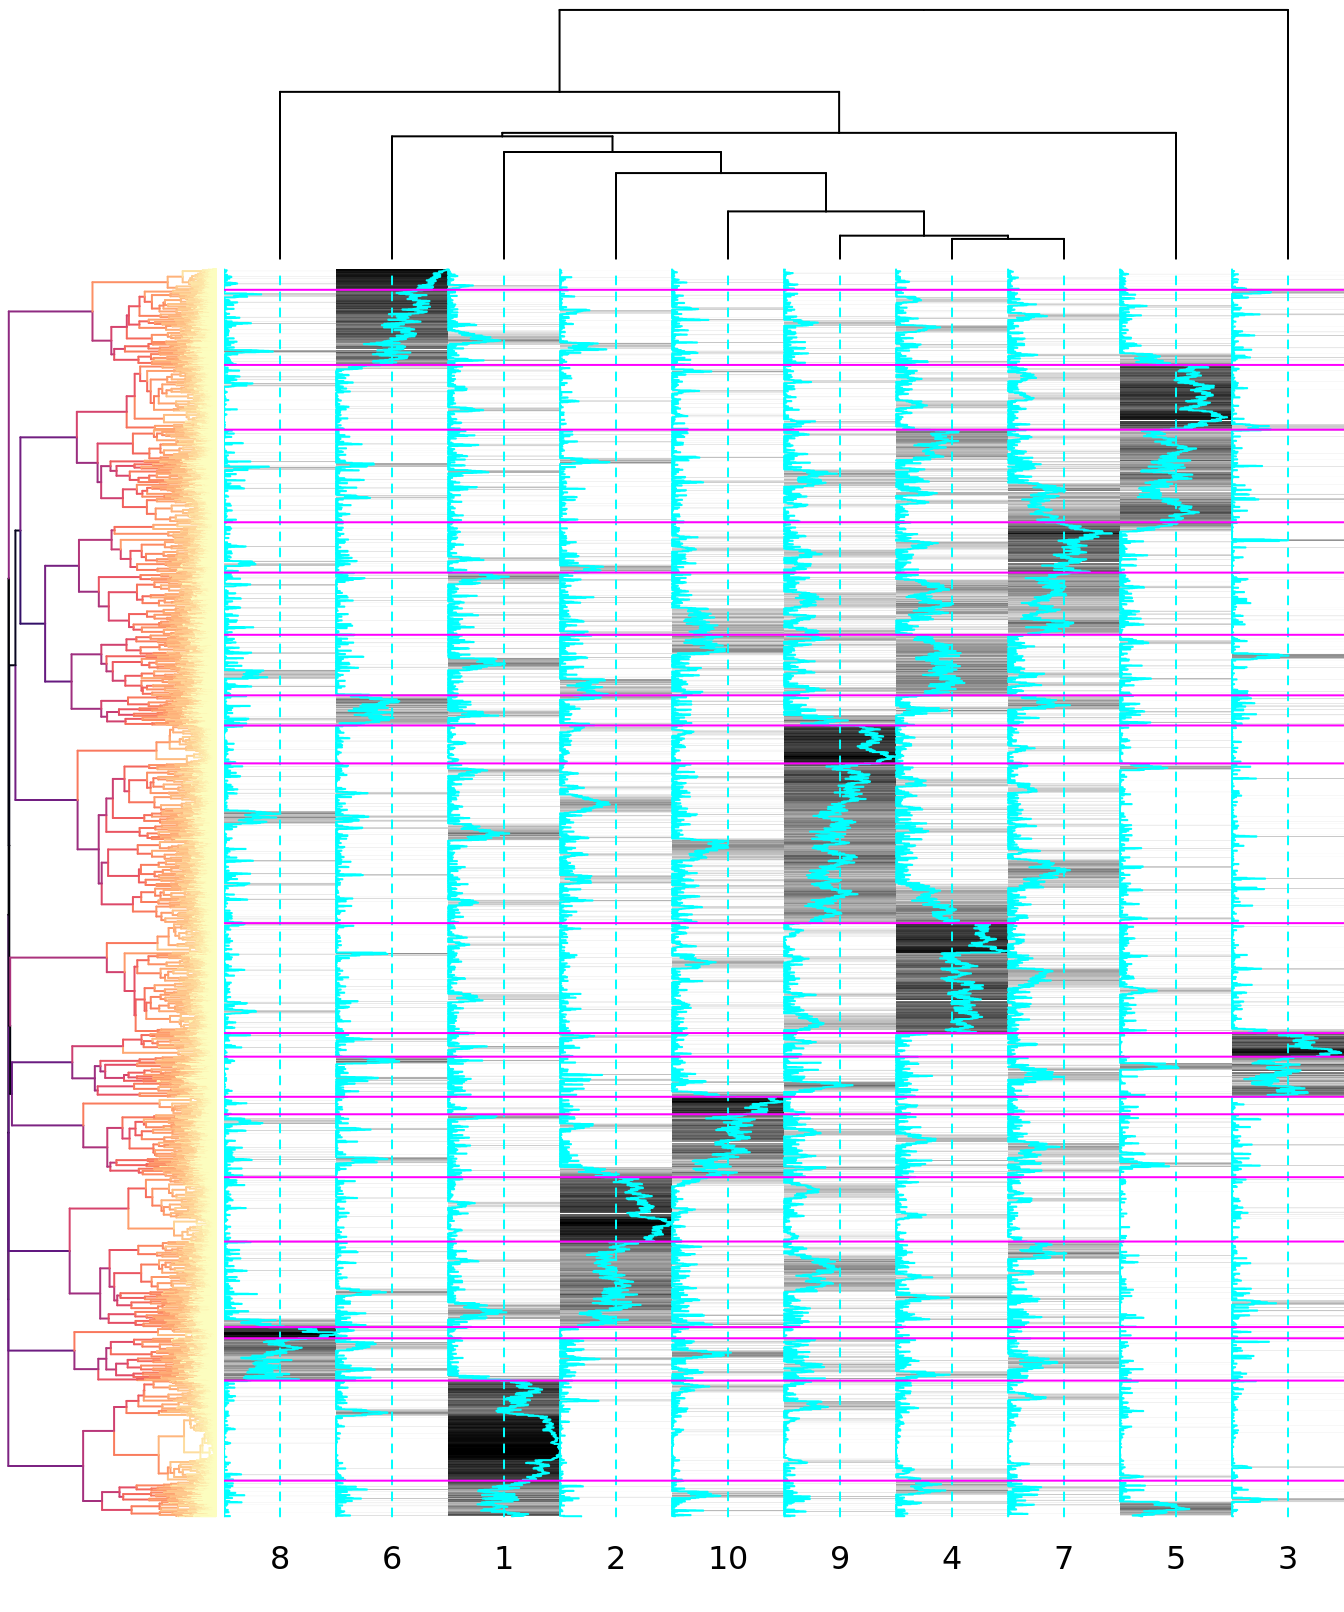
\includegraphics[width=0.9\linewidth]{ambrose_dissertation_files/figure-latex/hotleaf-1} 

}

\caption{Heatmap by optimal leaf sorting of documents (rows) and topics (columns)}\label{fig:hotleaf}
\end{figure}

A serial ordering is not a great fit to data that can be found in almost
any mixture, however it does reflect the human limitation that one must
read one thing at a time. As a seriation technique for reading the
ensemble hierarchical clustering model suggests a reading order of
starting on a spine to read bellwether texts, then choosing clusters on
the flanks to survey the combinations in which the focal topic is the
majority player. One would then move to a different spine and repeat the
technique. The order of spines can be taken from the height of their
leaves, starting low and working up to higher mergers. This would begin
the reading order with the topics that are most closely related. In this
case the lowest fork contains topics 4 and 7, though in a survey around
every spine the relationships to almost all other topics would be
addressed.

On the high side of the topic tree the most distant merges occur with
topics 8 and 3. Interestingly, whereas topic 8, French language, was
highly distinct looking only at terms, when looking at documents topic 3
is the most distinct. This makes sense under the theory that it is the
translated abstracts that are being pieced out by topic 8, and that the
rest of the documents if they are English must be composed of other
topics. Indeed the spine of topic 8 is very short and the majority of
its trace is below p = 0.5 and mixing with a variety of other topics. By
comparison topic 3, pan Asian culture, mixes mainly with topics 7
(gender), 9 (literature), and 6 (music). A slice of 3 mixes with 5
(film); because we presume 5 to be relevant to modern times it may show
that the content is not always necessarily about distant history as was
gleaned by the bellwether review.

Almost every cluster has some activity away from its spine, but these
tend to be minority players related to the spine of a different cluster.
Given this pattern, in which not only combination but proportion
matters, there may well be more strata than there are pairwise
combinations of topics. Assuming a modest five texts per stratum, a
lower limit of 45 topic pairs, and an upper limit of 90 to double that
so that each topic may be in a minor and major position, then we would
expect to read between 225 and 450 texts to be able to make a claim to
have understood the remaining 5,894 to 6,119.

This seriation method would fail only in the case of truly
unconcentrated clusters that are adjacent to no spine. The simplest
version would be three way relationships meaning that then even more
strata would be warranted. This scenario appears to occur three times in
this data set. The most important instance fills the space between the
spines of 9 and 7 where a middling cluster of topic 4 is mixed in a
variety of combinations. It happens again between 2 and 8 adjacent to
the spine of 2 but a separate cluster, and finally again between 9 and 4
adjacent but separate from 9. Thankfully the same model allows this
possible lacuna to be noticed and filled without worrying too much about
the combinatorics of three way interactions.

Though it may be an arbitrary simplification, a feature of the
hierarchical model is that we may choose a cut point to split the
dendrogram into a desirable number of groups. By trial and error 21
groups splits the tree into a major and minor cluster for each topic,
where the major component is the spine with probabilities close to one
and the minor are the different mixtures in which the topic is usually
dominant. The 21st slot accommodates an additional disjoint minor
cluster for topic 6. The boundaries of these groups are indicated by
magenta lines in the figure. Next we will discuss how to use these
clusters for stratified sampling.

\hypertarget{reading-strata}{%
\section{Reading strata}\label{reading-strata}}

Table \ref{tab:hottable} provides a numerical summary of Figure
\ref{fig:hotleaf} replacing documents with their clusters and tabulating
the number of documents in which a topic is dominant. The rows and
columns are in the same order as the figure. Treating these 21 clusters
as sampling strata is a more manageable research design than the above
mentioned 45 to 90 pairwise strata and reflect the empirical reality
that three way combinations are rare and that not all pairwise
combinations are important. They also narrow us to a research question
that is either diagnostic or substantive depending on what the
qualitative content of texts holds. The substantive question is, how
does the content of a topic change when discussed in isolation versus in
combination? The diagnostic question is, what happens to the content of
a topic when the when its documents are not well explained by the
available topic context.

The difference is that the former assumes topic validity, whereas the
latter make a different assumption about topic bias than we have
previously discussed. In our diagnostics we were concerned that the low
but nonzero probability terms of a topic by term vector represent
sources of error and bias, for instance, due to idiosyncrasy. This was
the body of the urchin. The problem with this kind of bias was that a
generalization from the spine to body may be inappropriate because
documents in the body actually represent classification errors and
should not necessarily be understood to belong to the same class as
their spines. Depending on the researcher's goals this body bias may not
have been too damning. If the topics that are learned are internally
valid, and it is easy to identify the documents that they validly
explain, then at least the researcher can claim to have understood some
important portion of the corpus even if there remains a substantial
unexplained portion.

Now we consider that it may also be possible that the spines are the
bias inducing portions of the corpus. The logic here is that a text
should never be categorized as nearly 100 percent derived from a topic,
because this implies that it is 100 percent generic, that is, totally
lacking in idiosyncrasy. What may be more likely is that those strongly
classified documents are the ones that happen to not share any overlap
with the other \emph{available} topics. Since they must be 100 percent
classified, in order for them to be classified anywhere the estimator
may choose to distort the term vector to make special dispensation for
these weird texts. This would imply that the texts that contain a
mixture of a topic, rather than those wholly derivative of a topic,
reflect the more valid portion of the term vector. If this kind of bias
is indeed operative, then it poses a problem to the researcher, who will
base her interpretation of a topic on the less valid portion of its
texts.

Our stratification approach will allow us to adjudicate the question of
validity by way of QCV. Each topic is represented by at least two
strata, one mixed and one unmixed. We may compare the content of the
unmixed texts to the topic portions of the mixed texts and assess
whether they indeed reflect the same content. If they do, then the
estimation is unbiased in at least this respect. If they are
substantially different, and the unmixed documents appear less topic
relevant than the mixed, then we have found a particular sort of bias
due to underspecification of K.

\begin{table}[!htbp] \centering 
  \caption{Document Clusters by Percentage Primary Topic Classification} 
  \label{tab:hottable} 
\begin{tabular}{@{\extracolsep{5pt}} lrrrrrrrrrrrr} 
\\[-1.8ex]\hline 
\hline \\[-1.8ex] 
Cluster & 8 & 6 & 1 & 2 & 10 & 9 & 4 & 7 & 5 & 3 & Total & N \\ 
\hline \\[-1.8ex] 
6 &  & 100 &  &  &  &  &  &  &  &  & 100 & 108 \\ 
6.1 &  & 97 &  & 1 &  &  &  &  & 2 &  & 100 & 382 \\ 
5 &  &  &  &  &  &  &  &  & 100 &  & 100 & 329 \\ 
5.1 &  &  & 1 & 1 &  & 1 & 12 & 11 & 74 &  & 100 & 471 \\ 
7 &  &  &  &  &  &  &  & 99 & 1 &  & 100 & 256 \\ 
7.1 &  &  & 5 &  & 9 & 3 & 21 & 62 &  &  & 100 & 316 \\ 
4.1 &  &  & 6 & 3 & 12 & 4 & 71 &  &  & 4 & 100 & 308 \\ 
6.2 &  & 52 & 5 & 5 &  & 20 & 7 & 11 &  &  & 100 & 153 \\ 
9 &  &  &  &  &  & 100 &  &  &  &  & 100 & 193 \\ 
9.1 & 1 &  & 2 &  & 3 & 77 & 10 & 6 &  &  & 99 & 812 \\ 
4 &  & 1 &  &  &  &  & 99 &  &  &  & 100 & 559 \\ 
3 &  &  &  &  &  &  &  &  &  & 100 & 100 & 120 \\ 
3.1 &  & 9 &  &  & 2 & 10 &  & 6 & 6 & 65 & 98 & 204 \\ 
10 &  &  &  &  & 100 &  &  &  &  &  & 100 & 89 \\ 
10.1 &  & 2 & 1 & 8 & 86 & 1 &  & 1 & 2 &  & 101 & 320 \\ 
2 &  &  &  & 100 &  &  &  &  &  &  & 100 & 327 \\ 
2.1 & 3 &  & 5 & 82 &  & 6 &  & 3 &  &  & 99 & 435 \\ 
8 & 100 &  &  &  &  &  &  &  &  &  & 100 & 57 \\ 
8.1 & 73 & 3 & 5 & 1 & 8 & 2 & 2 & 6 &  &  & 100 & 215 \\ 
1 &  &  & 100 &  &  &  &  &  &  &  & 100 & 509 \\ 
1.1 &  &  & 77 &  & 1 &  & 4 &  & 18 & 1 & 101 & 181 \\ 
\hline \\[-1.8ex] 
\end{tabular} 
\end{table}

Given the linear ordering of rows and columns, three seriation
approaches are possible. \emph{Inside out} would proceed from the lowest
to the highest leaves when assessing topic relatedness, the lowest in
this case being 4 and 7, and would emphasize the most interdependent
topics first. Conversely \emph{outside in} would start with the most
independent topics. Finally, the easiest \emph{playlist} seriation would
simply be to read in the order given choosing either the top or bottom
as a starting point.

We may now reflect on the guidance offered by Table \ref{tab:sumrnk},
where topics 6 and 9 had the best and topics 2 and 7 the worst
performance across a battery of diagnostics. The clustering results bear
the diagnostics out only in one respect. If good diagnostic performance
meant a strong signal then it makes sense that topic 6 is

Figure \ref{fig:gen-samp} illustrates the use of these clusters as
strata for a sampling approach to mastering a corpus defined by the term
genre. The clusters are seriated in playlist order from left to right
beginning with

\begin{figure}

{\centering 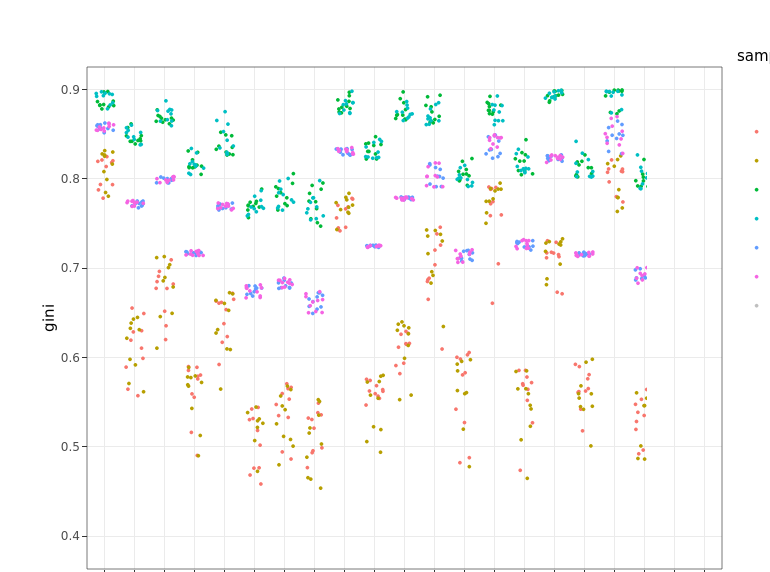
\includegraphics[width=0.9\linewidth]{ambrose_dissertation_files/figure-latex/gen-samp-1} 

}

\caption{Reading Strata and Sampled Texts.}\label{fig:gen-samp}
\end{figure}

\begin{figure}

{\centering 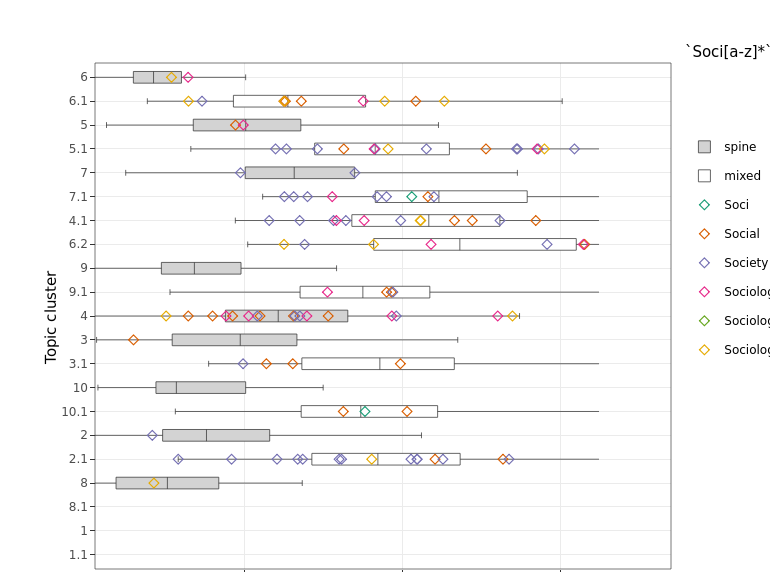
\includegraphics[width=0.9\linewidth]{ambrose_dissertation_files/figure-latex/sociology-1} 

}

\caption{Topic locations of sociology texts (n = 182)}\label{fig:sociology}
\end{figure}

\hypertarget{results-1}{%
\section{Results}\label{results-1}}

The first point concerns the urchin. Above we posited that it is in the
spines of the urchin that the essence of topics is found, and it is the
body that contains the idiosyncrasy. This is true for the good version
of a bad model, but it is likely that topic model estimators actually
find a different, worse version of a bad model. Consider the status of
horror in the film topic. Horror was a subgenre of film and it was
ranked very highly on the film topic, indeed horror articles were the
bellwethers. The reason was that the topic came to most strongly
associated with the component of it with the most distinctive
vocabulary. Drama, for example, which uses a less fantastic and more
relateable vocabulary, is drawn down the spine where it can mingle with
the topics to which it is connected. Why should the weirdest component
of a topic be treated as its most essential? This is a trend that all
underspecified topic models will exhibit.

The easiest way to test the expectation that perfectly classified
documents are actually biased upward by idiosyncracy is to look directly
at how the words they contain are classified. For clarity we assign
every term in a document to a single topic though it is technically a
distribution across all topics. A method to quickly accomplish this and
simplify the topic descriptions is to treat each document as a term by
topic matrix, project the matrix as a bimodal network, and perform the
Louvain community detection method described in
\protect\hyperlink{network-community-detection}{Chapter 2}. Within the
resulting clusters, which will contain terms and topics, we sort items
in decreasing order of their total probability, meaning the strongest
topics and most frequent terms will be listed first. Given these lists,
we can easily see whether the terms in a text assigned to a given topic
are really reflective of our theory of that topic.

Limiting ourselves to the social science subsample, let's compare the
most highly ranked music article, Henry's ``Social Structure and Music:
Correlating Musical Genres and Social Categories in Bhojpuri-Speaking
India'' (\href{www.jstor.org/stable/10.2307/836786}{\#6249}), which is
estimated to be 79 percent about music, with the lower ranked Rowe's
``Vitamin S: Messages, Music and Video--- an Analysis of the Sexual
Content and Perceptions of Sexuality Communicated in Popular Jamaican
Music Videos'' (\href{www.jstor.org/stable/10.2307/24384502}{\#3623}),
which is estimated to be 39 percent about music. Figure
\ref{fig:txt-com} plots some of the words from each of these texts.
Shown are the words for which topic 6 was their highest probability.
Note that several overlapping words are ommitted for legibility, so this
is illustrative of the content. Each of the words was inspected and
judged to be relevant to music, maybe relevant, and not relevant. In the
yes category are terms with a clear musical reference such as
performance, cultural, popular, and entertainment. In the maybe category
are words that are plausibly related to music but apper to refer to one
or more suppressed topics. Religious and youth, for instance, belong to
different domains even if they make sense in combination with music. In
the no category are words that are either idiosyncratic to the text
(like India and Jamaica) or are very general (like number and examples).
Words at the same vertical location contribute equally to the total
topic score for each text, and while the yes words have a higher mean
probability there is also considerable overlap with the less revelant
categories of terms.

\begin{figure}

{\centering 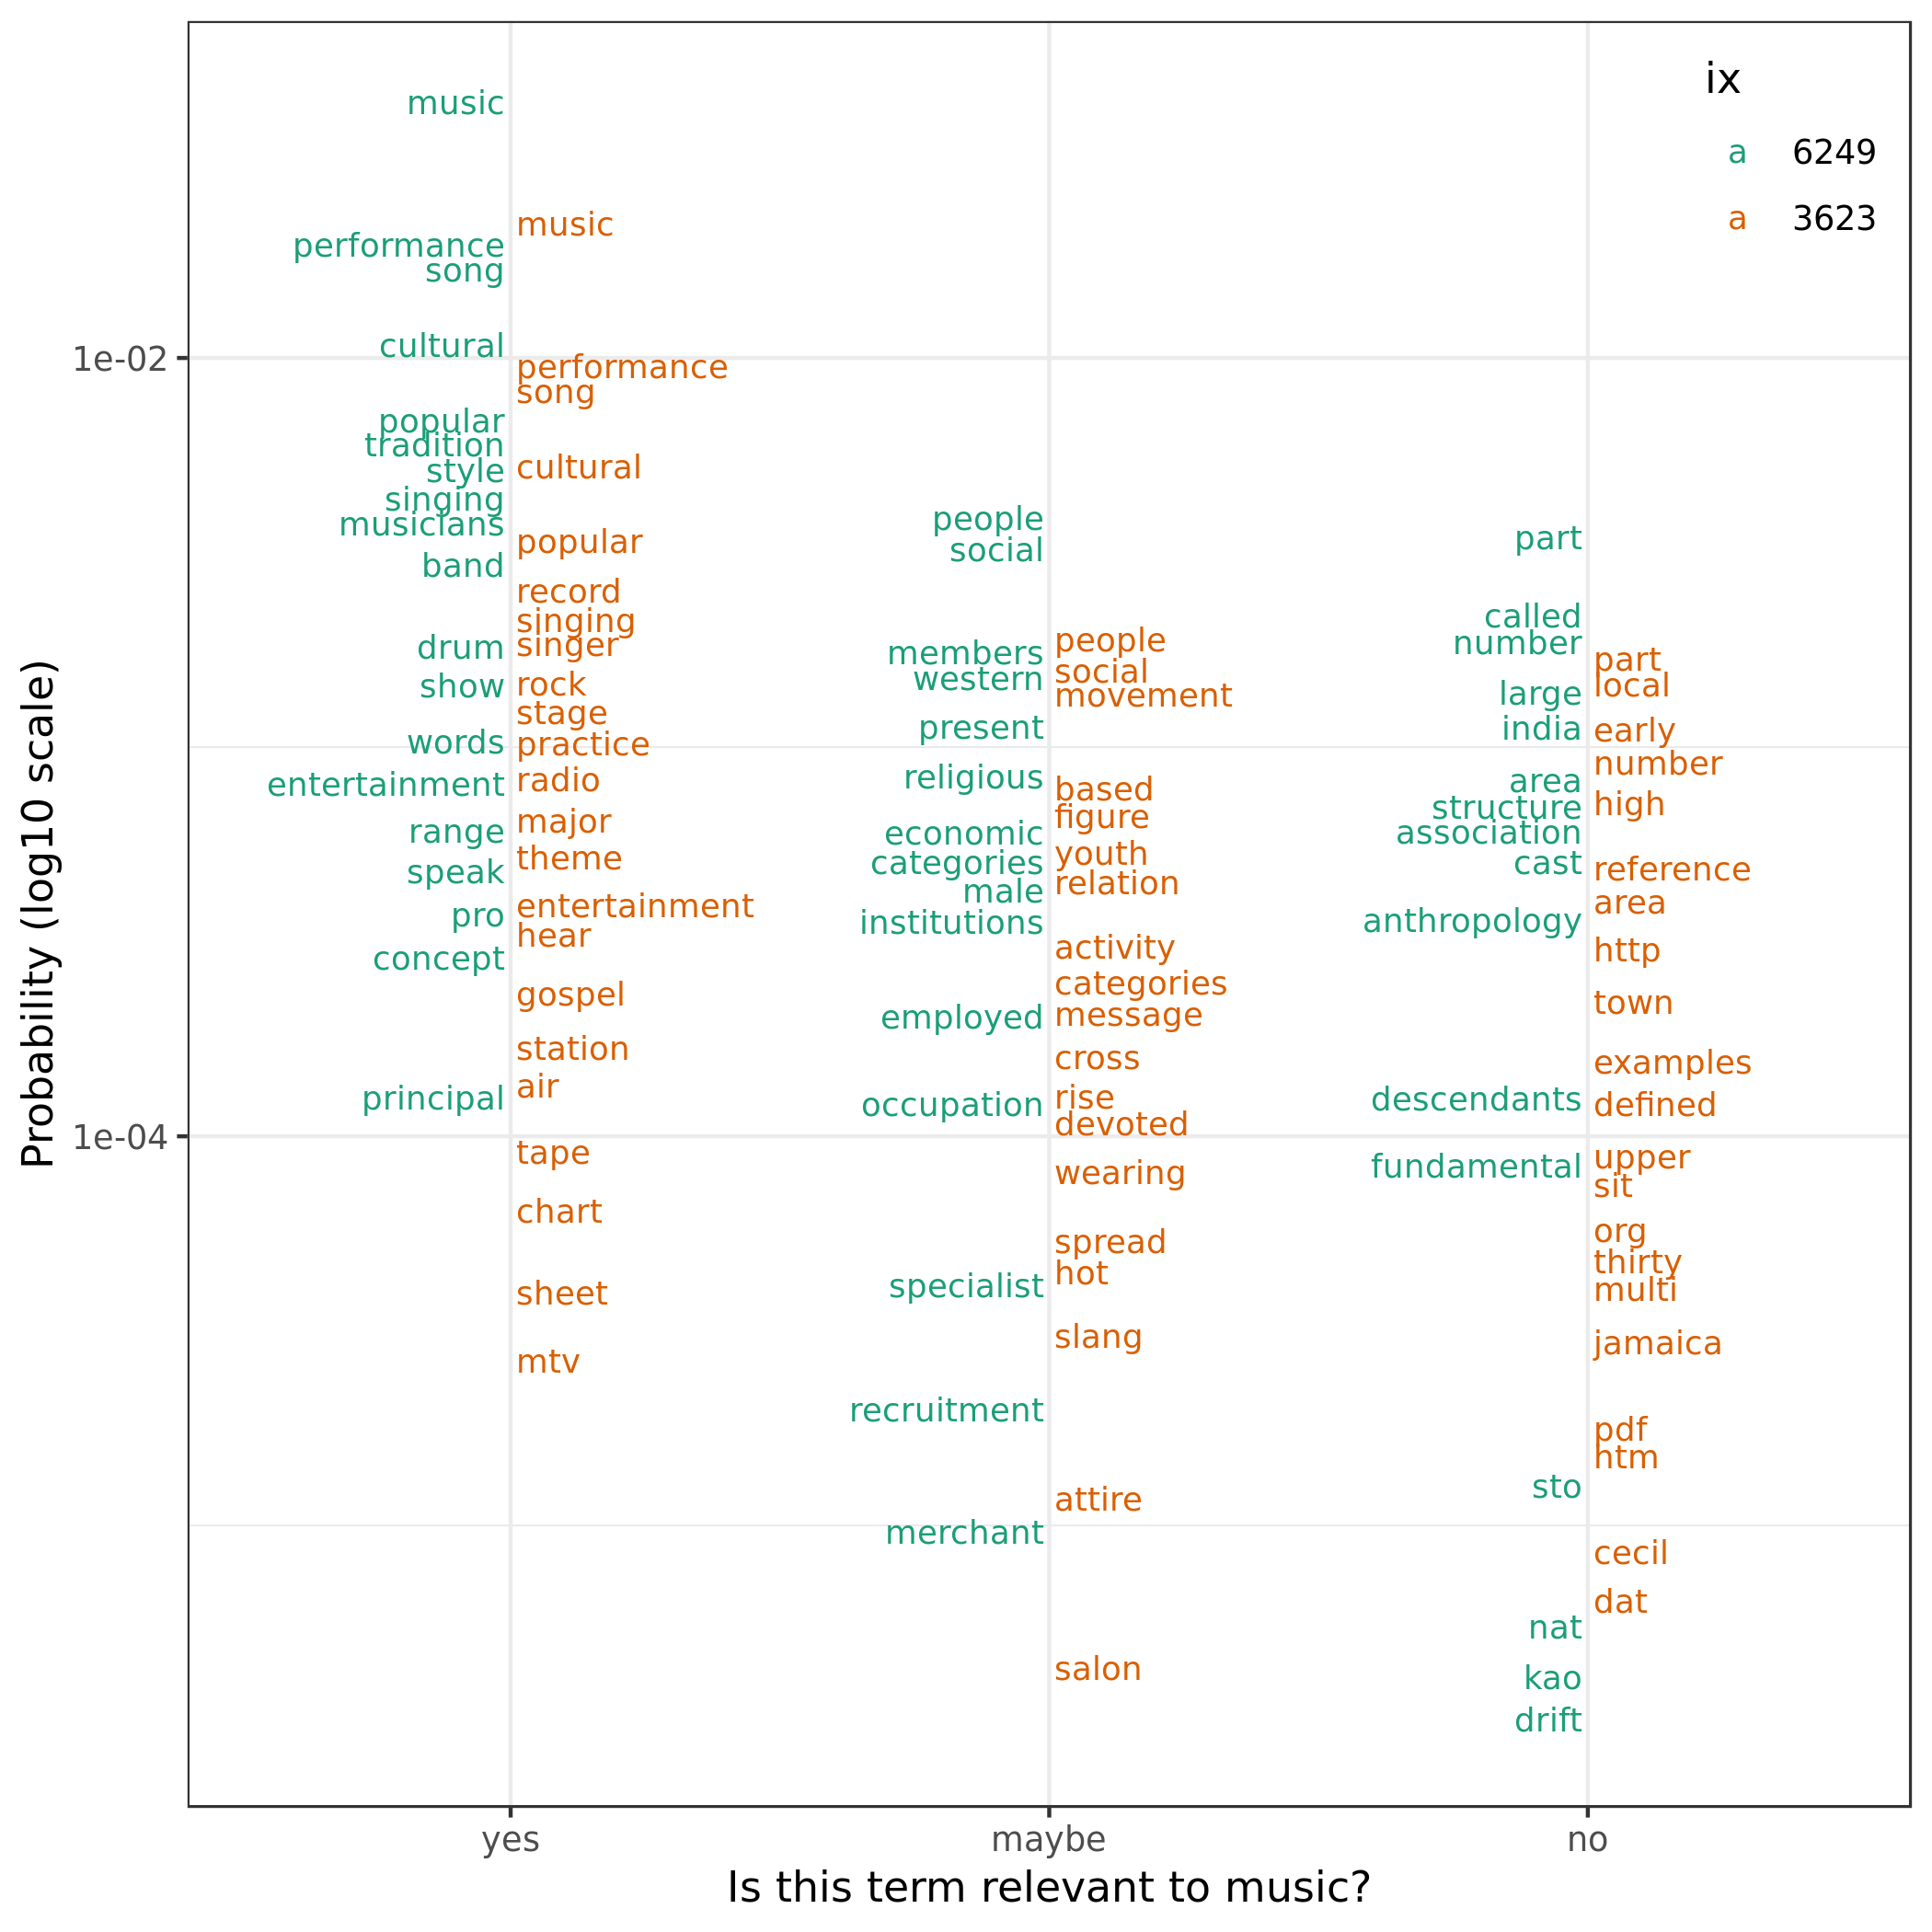
\includegraphics[width=0.9\linewidth]{ambrose_dissertation_files/figure-latex/txt-com-1} 

}

\caption{Terms estimated from music topic and present in text, by document probability and relevance to music. Document 6249 is 79 percent and document 39 percent about music. Some terms ommitted to prevent overlap.}\label{fig:txt-com}
\end{figure}

We may now test the expectation that the bellwether texts, those with
topic probabilites close to one, contain more classification errors than
mixed texts with weaker classifications. Table \ref{tab:txt-comt}
compares the sums of the probabilities for each text by the music
relevance categories. The estimated topic proportion of text 6249 is
double that of text 3623. The sum of probabilites of only the words that
actually appear in each text is much lower than the estimate; almost
three quarters of the estimate are ghost probabilities accruing from
terms that are not actually present in the text. Broken out by relevance
category, the true classification portion is slightly lower. In the case
of 6249, of the original 79 percent topic score, 17 are undeniably
relevant to music.

If bellwether texts had a higher rate of classification errors than
lower ranked texts then their percentage of false positives would be
higher. This can be seen in the number in parantheses, which
standardizes the left hand column to sum to 100. At least when comparing
these two texts, there appears to be no difference in the false positive
(no) rate, which for both is between 11 and 12 percent. To be sure would
require manual coding of a large number of texts, which is beyond scope
for the current project. Suffice to say that the issue of idiosyncracy
contaminating topic vectors is real and in these cases created a bias of
about ten percent of the estimated topic probability when considering
only terms present in the text. The proportions deriving from words not
in the texts accounts for a much larger portion of the bias.

\begin{table}[!htbp] \centering 
  \caption{Document percentage of music terms (percentage of music share) relevant to music.} 
  \label{tab:txt-comt} 
\begin{tabular}{@{\extracolsep{5pt}} lrrrr} 
\\[-1.8ex]\hline 
\hline \\[-1.8ex] 
  & 6249 &    & 3623 &     \\ 
\hline \\[-1.8ex] 
yes & 16.87 & (77.35) & 8.97 & (78.07) \\ 
maybe & 2.5 & (11.46) & 1.16 & (10.1) \\ 
no & 2.44 & (11.19) & 1.36 & (11.84) \\ 
Total & 21.81 & (100) & 11.49 & (100.01) \\ 
Topic Proportion & 79 &  & 39 &  \\ 
Adjusted Topic Proportion & 89 &  & 50 &  \\ 
\hline \\[-1.8ex] 
\end{tabular} 
\end{table}

Notwithstanding these prima facie quantiative findings, the content of
the no list for each text are not entirely comparable. Text 6249 is
about local markets for music in a state in India in the 1970s. The
vocabularly relating to Indian culture, including references to Hinduism
and Islam, found no home in another topic, even in topic 2 which is
ostensibly about religion, and so wound up being categorized along with
music. Text 3623 is about sexual imagery in Jamaican music videos. Save
for the term ``Jamaica'', the no list contains terms that have general
meanings. There is no obvious idiosyncratic content in its no list. The
unique quality of this text was its concern with HIV and sexual
behavior. Those medically relevant terms do not have a topic of their
own, but in this case the idiosyncracy was allocated to one this text's
other two topic assignments, either topic 5 (film) or topic 7 (women).
If in each text we find both a generic and a unique story, the topic
model is not designed to help us model the unique portion.

\hypertarget{voc}{%
\chapter{Vocabularies of Anthropology and Sociology,
1888-1922}\label{voc}}

\hypertarget{abstract-3}{%
\subsubsection*{Abstract}\label{abstract-3}}


Knowledge development of journals in sociology and
anthropology is measured as the change in topic prevalence over time.

\hypertarget{keywords-3}{%
\subsubsection*{Keywords}\label{keywords-3}}


sociology of knowledge, topic modeling, history of social
science

\begin{center}\rule{0.5\linewidth}{\linethickness}\end{center}

What were the ideas that predominated in the social sciences at their
formation as professions in the postbellum United States? What was the
course of their development over a generation of scholarship? In this
study I will answer these questions inductively through a reading of the
original journals in each discipline. Though the goal is substantive,
the methodological challenges of consuming a large quantity of text will
feature importantly in the story that unfolds. Along the way I will
demonstrate the usefulness of the computational distant reading that is
being explored in the humanities and how it can be combined with
traditional textual analysis for social science purposes. While
controversial in humanistic circles that emphasize the primacy of the
reader's novel interpretive work when consuming text, distant reading
fits comfortably within a social science epistemology that aims to
achieve an objective description of intellectual history. Indeed,
computational methods offer a useful backstop to the subjectivity of a
particular person's reading of history.

Computational text analysis (CTA) promises to automate a particular
slice of what hermeneutic methods accomplish. Hermeneutics claims that
through historical methods it is possible to reconstruct the
interpretive context of texts such that they can be understood in the
same way that contemporary historical actors understood them.
Establishing such context is a laudable yet arduous feat of historical
research to uncover the social and intellectual milieu of a particular
text. This is the gold standard approach, but one that restricts the
field to specialists with the training and resources necessary for the
undertaking.

Computers cannot study history in this way. What they can do, however,
is mine source material for limited kinds of contexts. The kind I am
concerned with below are the historical vocabularies that writers used
to construct texts in historical time. Vocabularies are glyphs without
grammar; they do not mean anything, but nothing meaningful can be said
without them in the present or in the past. They are the mediated form
of language, and in communicating with each other historical actors
leave traces that survive perfectly in time so long as texts themselves
survive.

While computers cannot read meaning in texts, and can barely recognize
it, they are almost as good as humans at recognizing the glyphs of
texts, and vocabularies are nothing but glyphs. What computers lack in
smarts, they make up in speed and memory. The quantitative scale of
their recognition makes for a qualitative shift because vocabularies can
be enumerated across immense corpora of texts. Immense, at least, by
human standards as there are limits to even computer memory and speed.
Yet such enumeration of texts into objective historical categories; this
is a profound resource for the intellectual historian. That one could
begin a reading with such context would be a transformative research
tool. Vocabulary enumeration, by which I mean simply the counting and
classifying of texts according to the vocabularies they contain, invites
a population studies approach to intellectual history. Where
sense-making is driven by comparisons, a reader's arbitrary combination
of texts is guaranteed to lead to anachronism. But if we can know that
texts are relevant to each other without knowing why, we have done some
small amount of hermeneutic work by supplying texts as historically
correct context to each other.

And even going so far as abandoning the project of reading texts in a
historically correct way, vocabulary enumeration can still lend
objectivity to a novel construction, a productive anachronism, of
textual meaning. Because vocabularies, the problems solved by computers,
are mathematically, algorithmically, or stochastically determined, they
may provide an immutable description of corpora that, like a map,
enables individual and collective exploration within a common framework.
Such maps may become the parameters of interpretive methods, which we
may use to surface and control some of our subjectivity.

\hypertarget{social-science-history-in-context}{%
\section{Social science history in
context}\label{social-science-history-in-context}}

Below we will attempt a distant reading of journals in the disciplines
of sociology and anthropology. First, however, it will be helpful to put
the development of these professions into some historical context. I
take a coarse view of national history as the history of wars because of
their downstream effects on government activity and institutional
investments. The first period is between the end of the American
Revolution (1783) and the end of the American Civil War (1865) and is
the national context for the origin of U.S. anthropology. The second
period is after the Civil War until the end of World War I (1918) and is
the context for the origin of U.S. sociology and of modern U.S. higher
education generally. Wars of territorial expansion are waged regularly
during both periods against native peoples and rival colonial empires,
and social research was always recruited to solve attendant problems of
population and to provide rationales for the relationships with and
understandings of conquered or would-be conquered people.

In the interwar periods the leading structural changes tended to be
economic. Where wars were ruptual moments that stalled development
across many sectors of society, the attendant growth of military
capacity also tended to lead to expansions of government,
infrastructure, and even education via the training remaining with
veterans. The trememdous strain on civilian life in terms of labor
shortages during the Civil War thrust women into labor roles outside of
the home, expanding the scope of their integration into the economy and
public life even after returning to domestic roles as traditional family
life was reconstituted. As the organizational form diffused the old
bases of trust in kinship networks were supplanted by mechanisms of
communication and control oriented toward formal procedures rather than
personal commitments \citep{Zucker1986Production}. This new kind of
trust was based in the perceived fairness of rules, procedures, and
contracts as well as in the new intermediary role of managers.

Drawing on economic historians and institutional theory Zucker
\citeyearpar{Zucker1983Organizations} has shown a secular trend in the
late 1800s through the 1950s of a transition of American labor from self
and often family-based employment to wage or salaried employment by a
firm. This great transformation stirred a number of related elements
that had been taken for granted. The population shifted from rural
toward urban, primarily by leaving agriculture and taking up salaried
employment. While before work was organized around individuals, it now
became organized around corporate entities \citeyearpar[Figure
3]{Zucker1983Organizations}. This shift started during WWI, with wives
going to work for munitions and aircraft factories in the cities. After
the war ended, politicians expected a reverse flow back to the rural
areas, holding up adjusting the counts for 20 years that determine how
many should be elected from each state to the House, but this reverse
flow never actually happened.

While institutional theory has classically focused on predicting
stability of norms (see especially DiMaggio and Powell 1983), the more
intriguing side of the theory focuses on processes that cause change
(see Zucker, AOM OMT Distinguished Scholar Lecture, Institutional Theory
at a Crossroad, delivered August 12, 2019). Calcified institutional
structure (hierarchical, codified) is particularly susceptible to sudden
redefinition, especially if the elements are interlinked so that one
change can easily spread.





\begin{figure}

{\centering 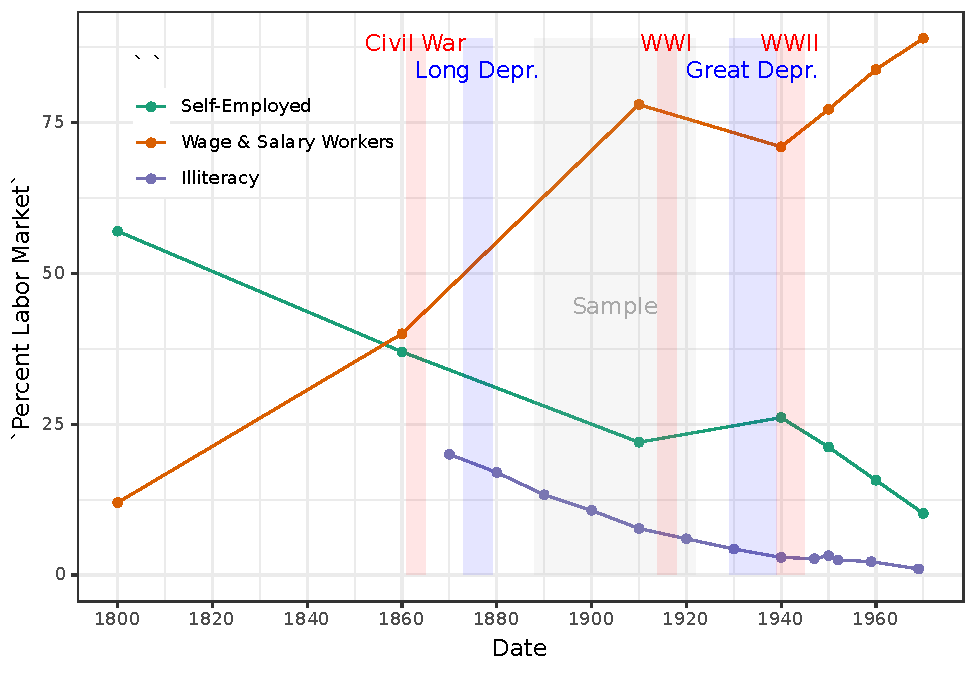
\includegraphics[width=0.9\linewidth]{ambrose_dissertation_files/figure-latex/zuck1-1} 

}

\caption{Shift from self-employment to wage-labor in United States.
Source: Table 4, Zucker \citeyearpar[15]{Zucker1983Organizations}.
Illiteracy Source: Table 6, Snyder \citeyearpar[21]{Snyder1993120}}\label{fig:zuck1}
\end{figure}

The use of procedural trust to organize production also heightened the
penalty to illiteracy; whereas orientations to personal loyalty and
family obligations were based in tradition and enduring social ties,
procedural trust required learning new relationships quickly in novel
on-the-job contexts. Contracts, manuals, bookeeping, and even posters
and signage on factory floors presumed what is now referred to as
functional literacy but was then still an emerging feature of
occupations. More quickly than in any other nation the literacy rate in
the United States rose due to public investments in education, fueled by
and fueling a growing demand for literate labor. Though early data for
earlier periods are unavailable, in aggregate personal consumer spending
on private education grew from 416 million dollars in 1909 to 1,170
million dollars in 1929, staying strong during WWI only to enter a
decline during the Great Depression. Consumer literate spending would
recover during WWII giving seeming unlimited opportunity for cultural
industries like publishing and education to turn the public's ability to
read into consumer demand and an engine for their own growth.







\begin{figure}

{\centering 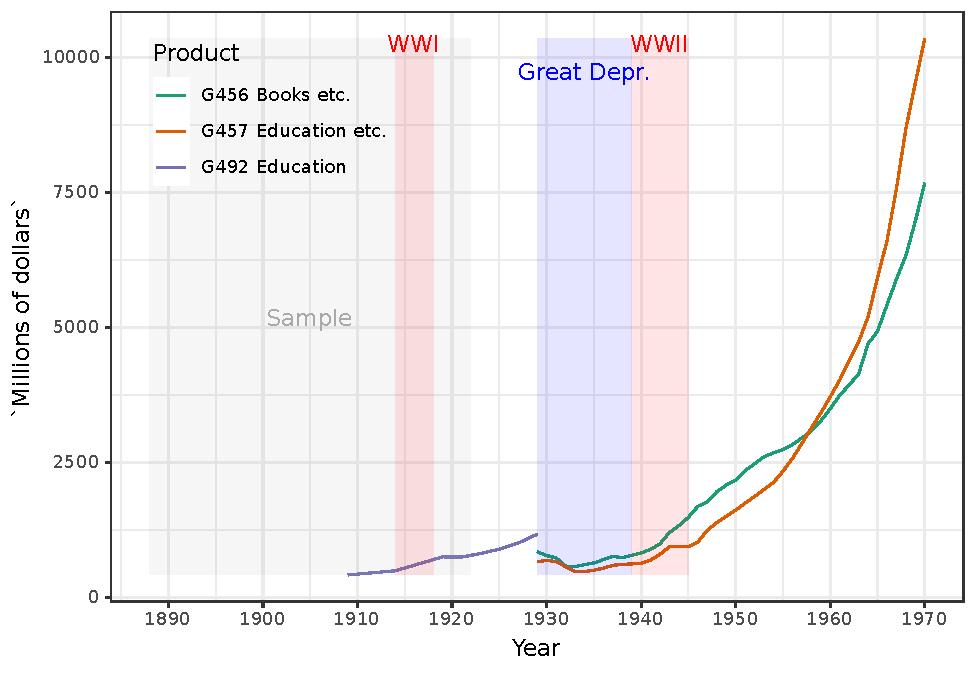
\includegraphics[width=0.9\linewidth]{ambrose_dissertation_files/figure-latex/per-con-1} 

}

\caption{Personal Consumption Current Dollar Expenditures on
Literate Products (``G456 Books, maps, magazines, newspapers, sheet
music'', ``G457 Private education and research'', and ``G492 Education
(private)''). Source: US Census Bureau
\citeyearpar[316-319]{Bureau1975Historical}}\label{fig:per-con}
\end{figure}

\hypertarget{kd-dq2}{%
\section{\texorpdfstring{ Social Science
Journals}{ Social Science Journals}}\label{kd-dq2}}

The most important journals in anthropology and sociolgy date from the
postbellum period, and the appearance of each is implicated in the
project of professionalization for each discipline. The 1920s marked the
end of war with the last of the militating American Indian tribes, and a
reckoning with the darkest sides of industrialization laid bare by WWI.
Social research had by this time completed a shift from colonial to
industrial problems and enjoyed a golden decade of development as a
profession, punctuated by the next great historical crisis in the Great
Depression. With the 1920s begins the adolescence of social research,
which is beyond the present scope. This study is of its childhood, which
ends with the Great War. I however draw the study out until 1922 because
it is the end of the public domain in U.S. copyright, to aid in the
reproducibility of the analysis and so that all readers may recover the
texts in question without difficulty.

The journals within social science cover five different subdisciplines.

\begin{table}[!htbp] \centering 
  \caption{JSTOR Social Sciences Journal Counts} 
  \label{tab:jclu-tab-sub} 
\begin{tabular}{@{\extracolsep{5pt}} lrrrr} 
\\[-1.8ex]\hline 
\hline \\[-1.8ex] 
Subdiscipline & N & Pct & Labeled & LPct \\ 
\hline \\[-1.8ex] 
Archaeology & 256 & 27.9 & 115 & 12.6 \\ 
Political Science & 219 & 23.9 & 183 & 20 \\ 
Education & 192 & 21 & 170 & 18.6 \\ 
Sociology & 160 & 17.5 & 145 & 15.8 \\ 
Anthropology & 46 & 5 & 89 & 9.7 \\ 
Population Studies & 22 & 2.4 & 27 & 2.9 \\ 
Geography & 18 & 2 & 32 & 3.5 \\ 
Transportation Studies & 3 & 0.3 & 7 & 0.8 \\ 
Total & 916 & 100 & 768 & 83.8 \\ 
\hline \\[-1.8ex] 
\end{tabular} 
\end{table}

\begin{figure}

{\centering \includegraphics[width=0.9\linewidth]{ambrose_dissertation_files/figure-latex/jbd-1} 

}

\caption{Birth and death rates for JSTOR journals, 5 year intervals.}\label{fig:jbd}
\end{figure}

\begin{figure}

{\centering 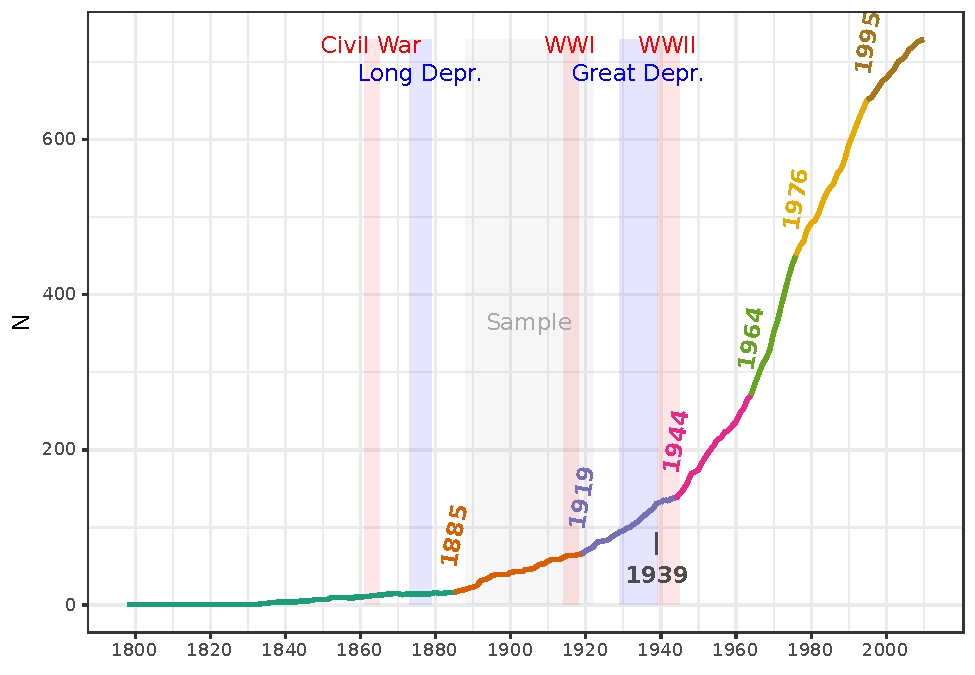
\includegraphics[width=0.9\linewidth]{ambrose_dissertation_files/figure-latex/jstorm2fig-1} 

}

\caption{Periods in the Growth of the Number of Social Science Journals in the JSTOR Archive}\label{fig:jstorm2fig}
\end{figure}

\begin{figure}

{\centering 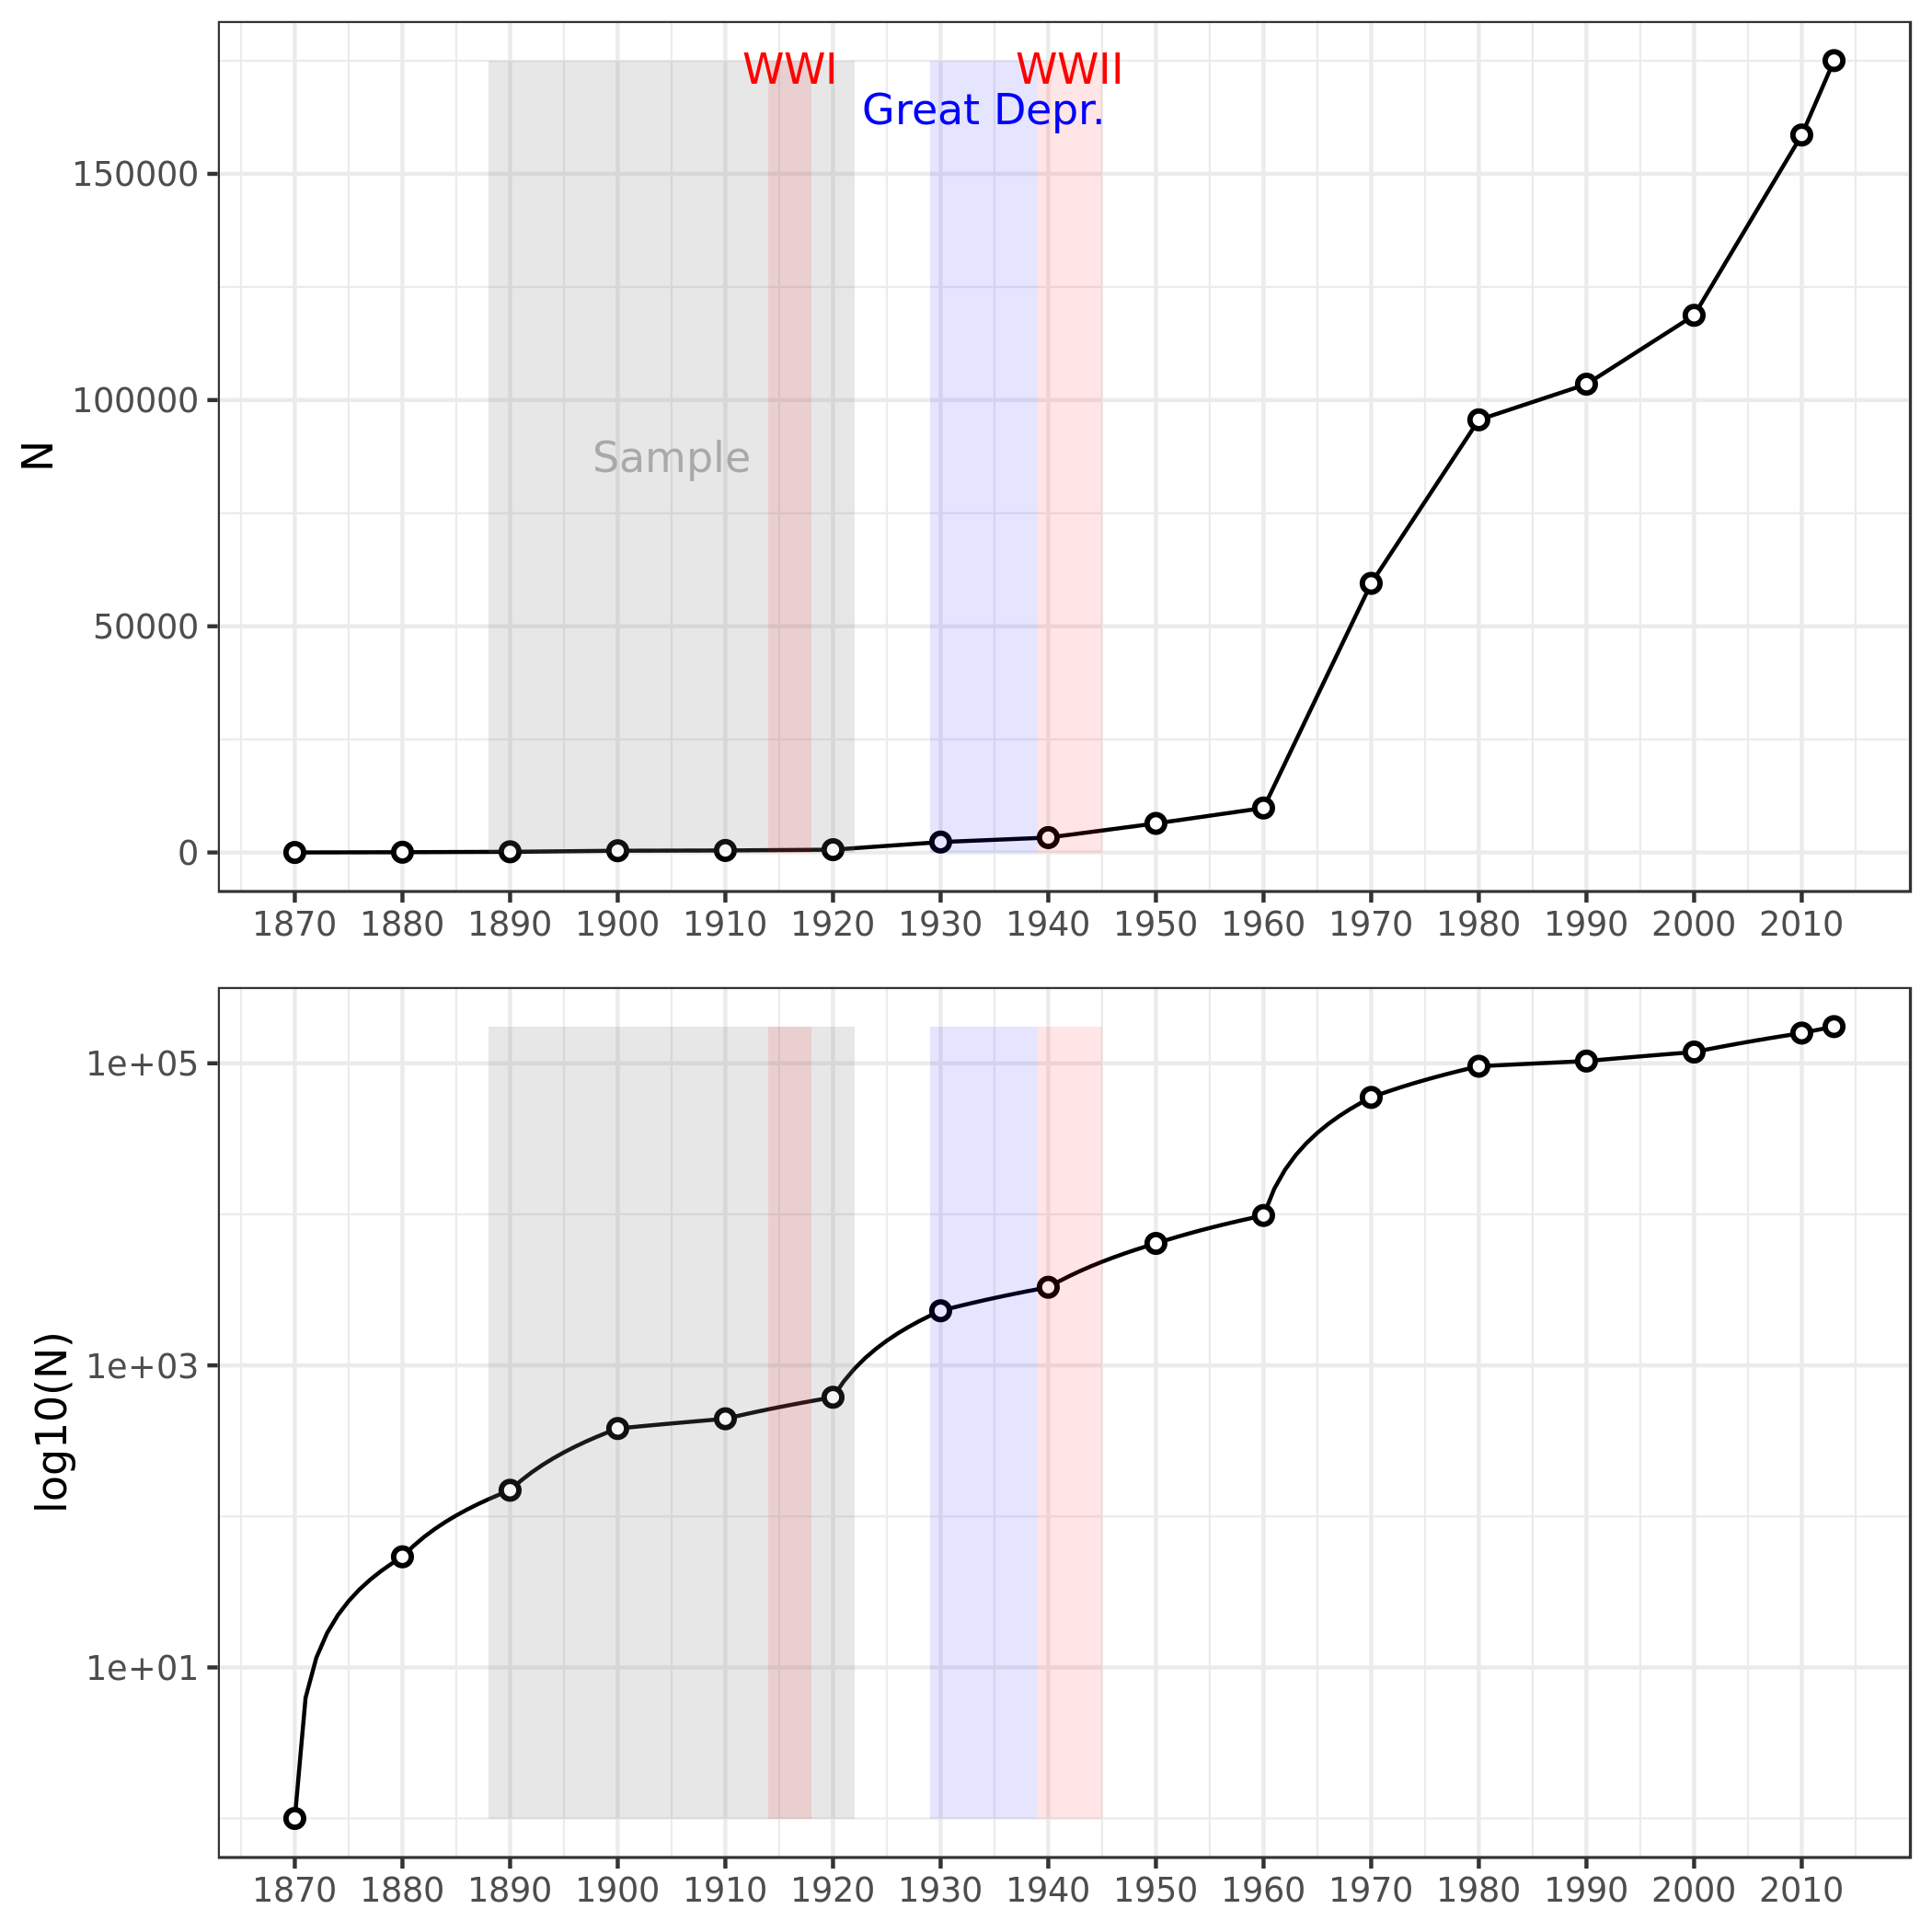
\includegraphics[width=0.9\linewidth]{ambrose_dissertation_files/figure-latex/nces2phd-1} 

}

\caption{Decennial growth in log10 of number of PhD degrees conferred in the U.S.}\label{fig:nces2phd}
\end{figure}

\begin{figure}

{\centering 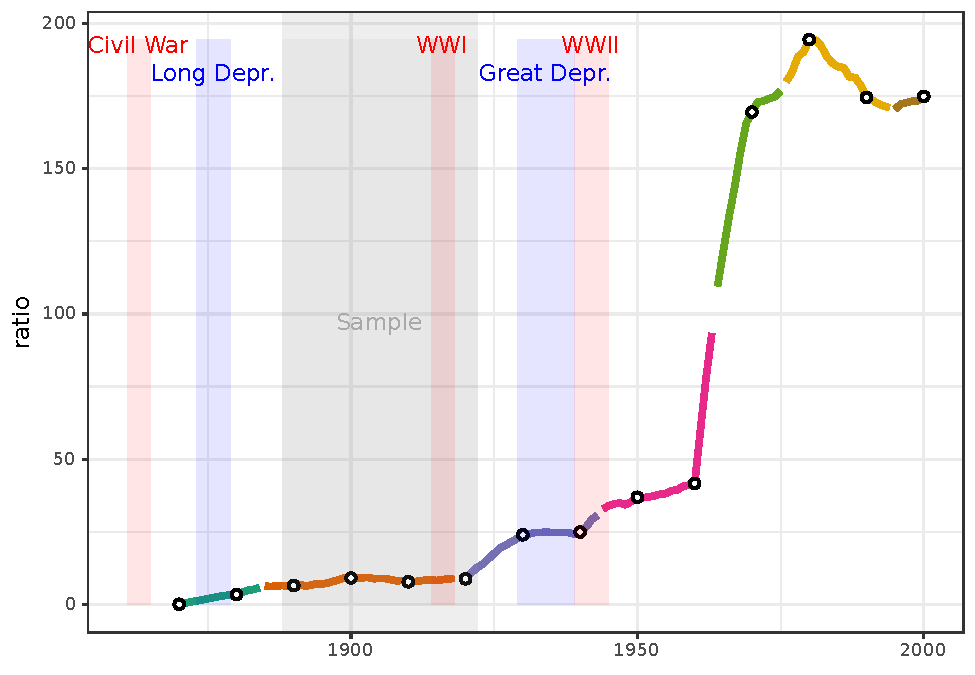
\includegraphics[width=0.9\linewidth]{ambrose_dissertation_files/figure-latex/nces/jstorm-1} 

}

\caption{Number of PhDs conferred in the United States per Social Science Journal}\label{fig:nces/jstorm}
\end{figure}

This period represents one of stable growth, as the size of the field
grows with the number of players on it. Between 1888 and 1922 there
tended to be about eight new PhD's in the U.S. for every social science
journal even as each population grew year over year. These growth
patterns begin to diverge around 1919 as a decades long acceleration of
personnel begins, relatively slowly between 1920 and 1960 at an average
acceleration rate of 28 PhDs per journal per year, and then quite
precipitously in the 1960s at an average acceleration rate of 147.

\hypertarget{topics-ideas}{%
\section{\texorpdfstring{ Topics \normalfont{≟}
Ideas}{ Topics  Ideas}}\label{topics-ideas}}

Given a relatively stable epoch in American society, one free of the
most extreme exogenous shocks of war and economic depression, how is it
possible to trace the development of the discursive structures of
American social science scholarship? I will use the digitized texts of
articles taken from social science journals in the JSTOR archive to
represent a time series of discourse. The methodological challenge is
how to count such an empirical source as text, which seldom considered
to be data at all.

Texts are after all for reading rather than counting. Above we have
shown how counting is possible within certain categories that are given
historically, namely the journal sources of texts. Theoretically,
however, there is a concern that discursive formations appear as a
conversation among texts that may not be visible in exterior labels, or
at least that such social or institutional labels are lagged behind
their cultural origins, if indeed they ever break through from the
cultural to the social. A genre category is the example par excellence
of a socialized culture, one whose relevance to a society at large,
however narrowly society may be conceived, is at least debateable
because it is visible in the language as a category. The conjecture here
is that direct analysis of texts may reveal the cultural currents, as
Durkheim referred to them, before the crystalize into firmer social
formations.\footnote{``To master the whole meaning of the discovered
  truths and to understand all that is summarised in them, one must have
  looked closely at scientific life whilst it is still in a free state,
  that is, before it has been crystallised in the form of definite
  propositions.'' \citep[\textbackslash299]{Durkheim1893division}}

To do that kind of counting at scale does require a humble approach to
text. Text is the bearer of meaning when read by humans. When read by
machines text are impoverished. Rather than claim to have access to the
meanings of texts, I instead make the more conservative claim to have
access to the vocabularies with which those meanings are communicated.
Thus the strategy of the study occurs in four steps.

\begin{enumerate}
\def\labelenumi{\arabic{enumi}.}
\tightlist
\item
  Sort text into categories of similar vocabulary.
\item
  Describe the vocabularies that define category membership.
\item
  Describe vocabulary prevalence across time and discipline.
\item
  Validate category contents by a traditional qualitative reading of
  texts.
\end{enumerate}

I will spend considerable effort on solving the problem presented by
step 1, as here everything depends on the computational methods
employed. Steps 2 and 3 are straightforward given a successful
mathematical model of texts. Step 4 is seldom attempted, and may be the
hardest of all, because it is here that machine and human learning must
be integrated. If I am successful, if through these steps I may
operationalize the notion of cultural meaning or cultural logic as
conformity to vocabularies, then I believe a new horizon of intellectual
scholarship is possible. If on the other hand I find that
machine-learned vocabularies do not correspond to human-learned
understandings of the texts drawing on those vocabularies, then the
discovery will be negative, that distant reading is not a scientific,
historical, or hermeneutic method, but rather a toy at worst and a best
new humanistic method of reading texts de novo.

As mentioned, the statistical tool I will rely on in step 1 is called
topic modeling, which refers to a variety of computational approaches to
text data that blur the distinction between qualitative and quantitative
analysis. The topic model paints a lexicographic picture of texts,
analogous to the demographic picture gained by a civil census survey of
cities and towns. To a topic model, texts are merely collections of
terms (usually words) that are counted to create the so-called ``bag of
words'' description of a text. In the same way that a census reduces
communities to counts of the names of people who live in them, topic
modeling reduces texts to the frequency of word choices in texts, to
their diction or vocabulary. Just as a census of people fails to capture
the nuanced interactivity of human settlements found in their culture,
politics, and economic activity, the topic model washes away the
meanings and intentions behind the words that are enumerated.

A population census would not be very helpful were it only a count of
the names of respondents, and of course the really helpful data derive
from the demographic and economic survey attached to the name. Text data
do not usually come with such a collection of rich covariates, yet
nevertheless topic models promise to discern helpful patterns from
counts alone. The trick behind the estimation of a topic model is that
it attempts to learn the demographic information (topics) without
asking, by merely looking at how the names alone (terms) are distributed
across geographies of interest (texts). If it can keep its promise, a
topic model applied to census data might recover the cultural patterns
latent in the distribution of names. It might, for instance, learn
different groupings of names that in turn correspond to markers like
age, race, national origin, or gender, so long as membership in those
categories was related to geography. It might, for instance,
successfully separate a category of Hmong names out from among the names
of all people living in St.~Paul because the non-Hmong names appeared in
other regions where no Hmong names appeared.

To call the category of names ``Hmong'' requires an interpretation of
the model, which by itself is just lists of names. This is the work of
step 2, and requires a little bit of shoe leather by trying to make
sense of what a list of names refers to. Here reading texts is like a
census taker knocking on a door, and a topic model's latent analysis
saves on this effort. Sometimes bringing domain knowledge to bear on the
list itself will suggest a category label, but often choosing a small
sample of texts as exemplars of the category. Still this requires much
less shoe leather than a traditional qualitative analysis in which each
text is studied directly. Of course the census is much more informative
because it asks about demographic categories directly thereby avoiding
the need for a latent analysis. In domains where rich covariates are not
yet available or are prohibitively expensive to acquire, latent analysis
provides promising clues of patterns that already exist. What is even
more interesting, and something that might surprise even census
analysts, is when latent categories do not correspond to known survey
items. In either event the power of topic modeling for inductive
analysis is to reveal structure in how names hang together that was
hidden.

Even without conducting the second labeling step, in step 3 it will
already be possible from the output of the model to inspect the
distribution of topics across available covariates, especially time.
These are the patterns that will help validate the topic models against
what is already known about intellectual history. For instance, the
power of institutional and generational change may well be apparent in
the historical distribution of topics. This step leads naturally into
step 4 by suggesting anomalies that can only be explained by a closer
look at the texts, the chore that the entire preceding analysis punts
on. In step 4 we learn either that our understanding of history was
wrong, or that our topic model was wrong, and there may be no method
other than one's judgement to decide.

\hypertarget{full-text-archive}{%
\section{Full-Text Archive}\label{full-text-archive}}

Computational text analysis requires that text corpora be transformed
from a human to a machine readable format. Several efforts to digitize
paper archives have made historical research designs possible, notably
the Google Books project, HathiTrust, and ITHAKA JSTOR archive. Digital
storage devices like the portable document format (PDF) have also
enabled texts to be represented in both a digital version and as a
reasonable facsimile of paper originals. Reasonable, we should say, for
most sociological purposes, put not for other historical questions where
materiality of culture is important.
\citep[149]{Schreibman2014NonConsumptive}

Digital archives make research into the production of culture difficult,
precisely because they misrepresent several aspects of the means of
production. Because researchers should be mindful that digitization of
texts abstracts some qualities of texts and renders many others
invisible. The importance of physical space and material qualities of
libraries is illegible when working with digital archives, while the
verbal content of texts is highlighted. We must keep in mind that we are
not viewing what historical actors saw. Digital texts are almost
perfectly fungible, while, variability in historical texts. We are
liable, for instance, to underestimate the search costs to locate texts,
and the fungibility of texts themselves.

Simply put, if the texts we analyze are not the ones that historical
actors read, can we be said to really be doing something historical?
There are reasons to believe that digital text archives provide not just
a useful but an historically valid abstraction from the material texts.
If we want to understand how an individual scholar understood a
particular text, better to have her personal copy, margin notes and all.
Yet how would that scholar have treated the text as a cultural item? She
would abstract her own copy to a format credibly held in common, the
more antiseptically clean version that we see in digital archives. These
are the ghosts of the texts, so to speak, but they are what would be
left when all idiosyncrasies were removed, the version that one would
assume colleagues thought of when declaring that text publicly.

This is by way of saying that the texts I compile below are not the same
that were read by the historical actors under consideration. They are
the texts that historical actors would assume their contemporaries were
reading, that is, the sanitized, fungible, original published form of
the text. By getting at these texts, we are getting at the real
historical infrastructure for scholarly communication.

\hypertarget{kd-dd}{%
\subsection{Data}\label{kd-dd}}

The optical character recognition that computers require in order to
store text digitally depends critically on the hard work of creating
quality scans of journal archives. JSTOR has done a commendable job of
this. Next we will describe what the JSTOR archive has to offer. Every
record for every journal was downloaded manually, including front and
back matter, articles, and book reviews.

\begin{figure}

{\centering 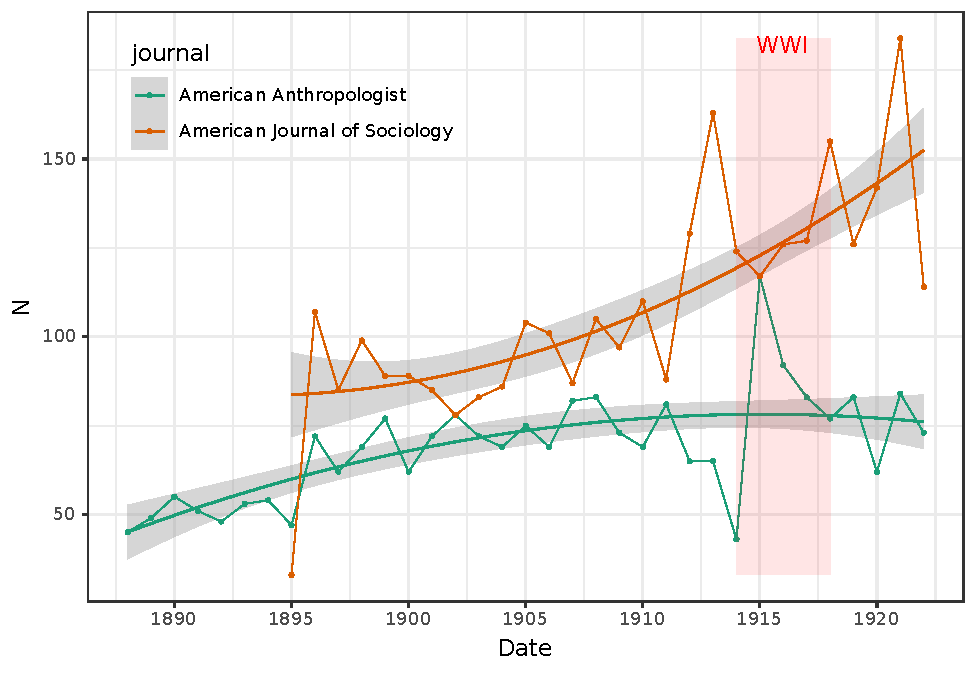
\includegraphics[width=0.9\linewidth]{ambrose_dissertation_files/figure-latex/jdpf-desc-1} 

}

\caption{Annual count of journal issue contents.}\label{fig:jdpf-desc}
\end{figure}

\hypertarget{kd-dp1}{%
\section{Sampling}\label{kd-dp1}}

\begin{figure}

{\centering 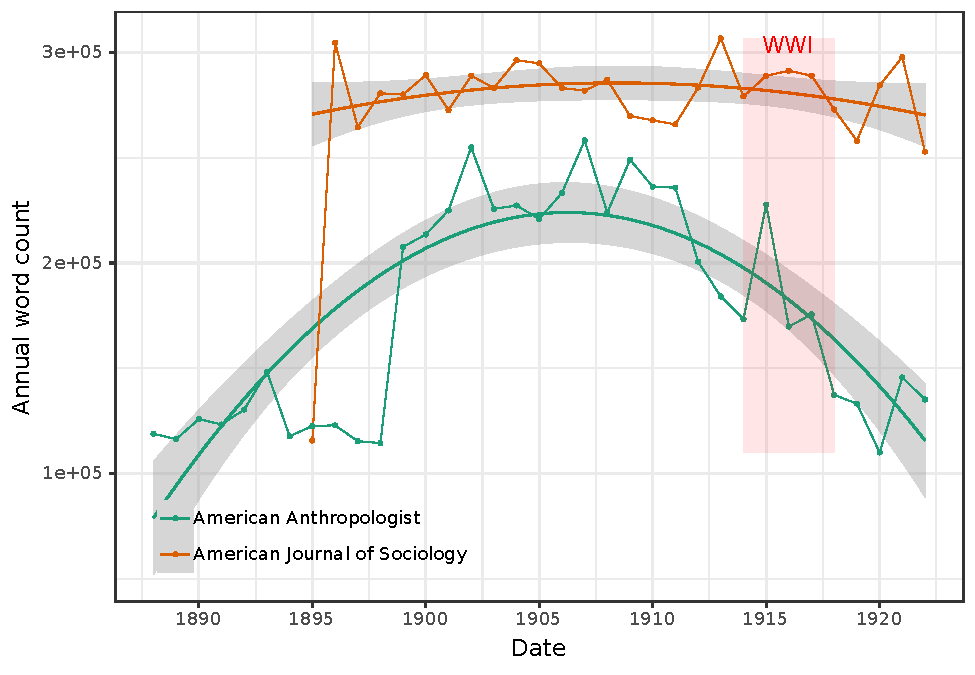
\includegraphics[width=0.9\linewidth]{ambrose_dissertation_files/figure-latex/pre2ntok-1} 

}

\caption{Total word counts of all issues of all journal contents annually.}\label{fig:pre2ntok}
\end{figure}

\begin{table}[!htbp] \centering 
  \caption{Filtering due to Data Management} 
  \label{tab:filt} 
\begin{tabular}{@{\extracolsep{5pt}} lrrrrrrr} 
\\[-1.8ex]\hline 
\hline \\[-1.8ex] 
step & doc & pag & par & sen & tok & ter & lem \\ 
\hline \\[-1.8ex] 
imported & 100 & 100 & 100 &  &  &  &  \\ 
cleaned & 99.27 & 98.21 & 67.51 &  &  &  &  \\ 
tokenized & 99.27 & 98.21 & 67.51 & 100 & 100 & 100 &  \\ 
preprocessed & 99.27 & 98.01 & 67.35 & 91.38 & 42.21 & 35.74 & 100 \\ 
sampled & 1.84 & 1.56 & 1.17 & 1.43 & 0.62 & 4.95 & 20.86 \\ 
100\\% & 5444 & 47596 & 232085 & 818183 & 19983852 & 326889 & 31963 \\ 
\hline \\[-1.8ex] 
\end{tabular} 
\end{table}

\hypertarget{units-of-analysis}{%
\section{Units of Analysis}\label{units-of-analysis}}

Conventionally researchers feed entire documents into the construction
of term frequencies. This method treats any term in a document as being
related to any other term by the same degree. The goal of any topic
mixture model algorithm is to sift these terms into different topic
categories basically by looking for clues across documents; a topic can
be ``seen'' in a particular document to the extent that other documents
include that topic and \emph{other} topics different from the focal
article, so that the intersection of terms reveals the topic. But a much
simpler assumption to reduce the attendant noise within a document is to
merely feed lower level syntactic structures--paragraphs and
sentences--to the algorithm. We will see that doing so greatly improves
the usefulness of discovered topics.

The irony of this approach is that while topics become more clear as
documents become shorter, the assignment of any particular shorter
document to a topic is murkier due to the smaller word count.

Long documents will contribute more text to the corpus, but this is fair
as they make up more of the population of text. Thus a simple random
sample will allow better descriptive statistics. I sampled at the
paragraph level because.

\hypertarget{how-many-topics}{%
\subsection{How many topics?}\label{how-many-topics}}

\begin{figure}

{\centering 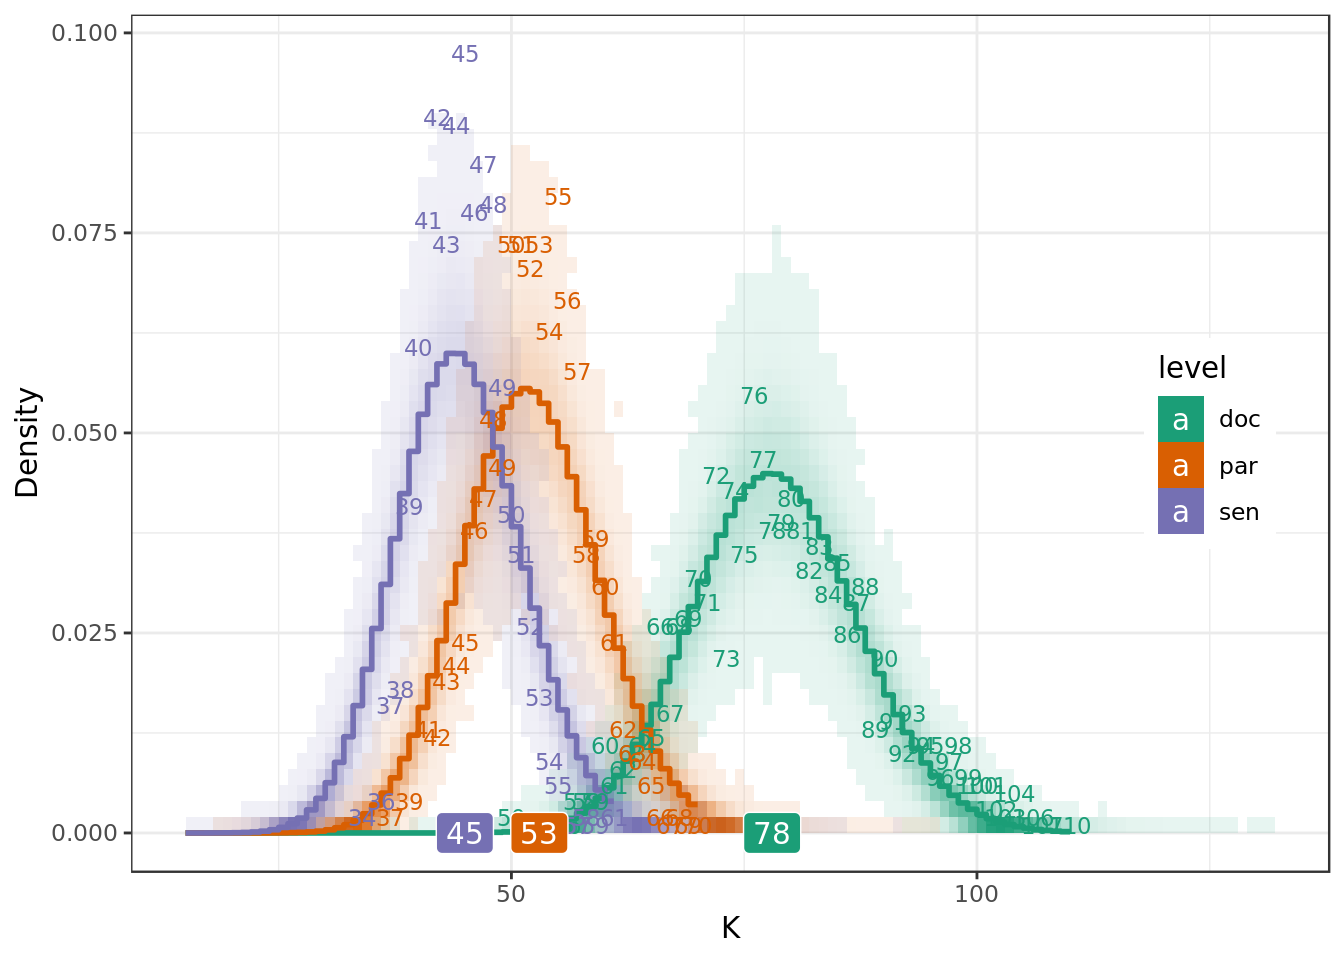
\includegraphics[width=0.9\linewidth]{ambrose_dissertation_files/figure-latex/sim-fig-1} 

}

\caption{Distribution of K by convex hull}\label{fig:sim-fig}
\end{figure}

\begin{table}[!htbp] \centering 
  \caption{Kurtosis Permutation Test} 
  \label{tab:mlk2k} 
\begin{tabular}{@{\extracolsep{5pt}} lrrrrr} 
\\[-1.8ex]\hline 
\hline \\[-1.8ex] 
level & e & se & l99 & u99 & P(e ≦ 0) \\ 
\hline \\[-1.8ex] 
doc & -0.0932 & 0.1149 & -0.3682 & 0.2252 & 0.7948 \\ 
par & -0.1125 & 0.1206 & -0.3999 & 0.2185 & 0.8257 \\ 
sen & 0.0118 & 0.2304 & -0.5078 & 0.6471 & 0.4973 \\ 
\hline \\[-1.8ex] 
\end{tabular} 
\end{table}

\begin{figure}

{\centering 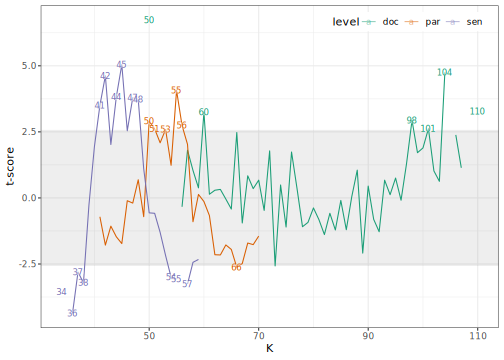
\includegraphics[width=0.9\linewidth]{ambrose_dissertation_files/figure-latex/mlk-tab-1} 

}

\caption{Significant Counts of K}\label{fig:mlk-tab}
\end{figure}

\hypertarget{topic-interpretation-1}{%
\section{\texorpdfstring{ Topic
interpretation}{ Topic interpretation}}\label{topic-interpretation-1}}




\begin{figure}

{\centering 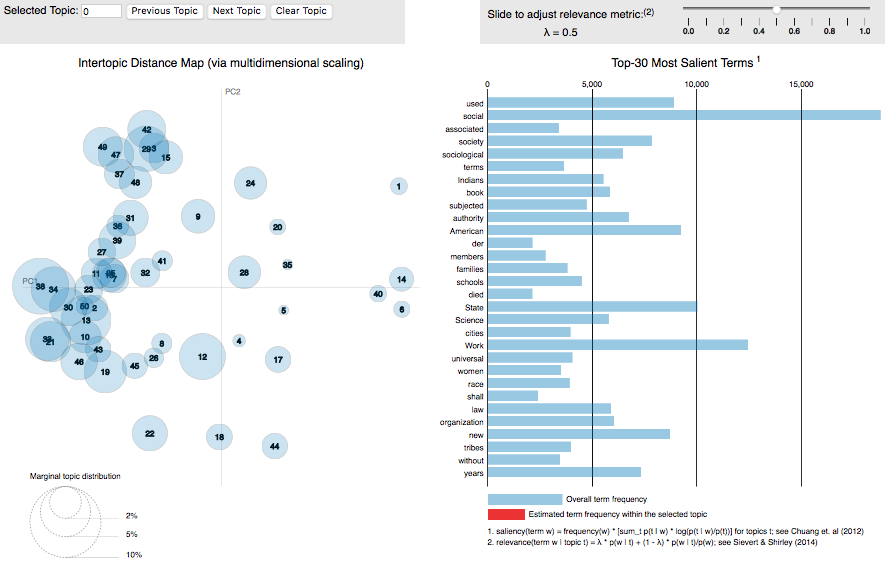
\includegraphics[width=0.9\linewidth]{img/soc-mod-viz} 

}

\caption{Topic Term Explorer, K=50.
\href{exh/viz/index.html}{\emph{Interactive pop-out.}}}\label{fig:soc-mod-viz}
\end{figure}

\hypertarget{cit}{%
\chapter{The Social Science Citation Landscape, 1900-1940}\label{cit}}

\hypertarget{abstract-4}{%
\subsubsection*{Abstract}\label{abstract-4}}


Knowledge mapping of academic journals promotes the
conservation of intellectual history and stimulates discovery of
underexplored intellectual opportunities. Treated as a large network
community detection problem, I demonstrate how to apply the clique
percolation method to map two kinds of recorded knowledge: citations and
full text. The features of generated maps are explained, and
interpretive methods including visualization are presented. We use
American social science scholarship in the first third of the 20th
century prior to U.S. entry into World War II as a case, and describe
how the intellectual landscape of four separate social science
disciplines developed.

\hypertarget{keywords-4}{%
\subsubsection*{Keywords}\label{keywords-4}}


citations, k-clique communities, community detection,
landscape

\begin{center}\rule{0.5\linewidth}{\linethickness}\end{center}

\hypertarget{wok}{%
\subsection{Mapping Knowledge Terrain}\label{wok}}

There are two reasons to map knowledge spaces. First, we may want to
know how knowledge develops as a resource unto itself. Second, we may
want to exploit such a map for a productive purpose. Here we will
attempt the second as prologue to the first. We will tackle the
technical problems of constructing a map. We will show how a map can be
put to use. Finally, we will investigate how the particular map we make
may tend to predictably get us lost.

All knowledge mapping requires first an ontological and then an
analytical action. Ontological actions delineate the things that matter.
They arbitrarily construct from perception the items that we then think
about. While ontological decisions tend to define the scope of
everything that may be learned from an investigation, they are often
assumed rather than demonstrated. Actor Network Theory (ANT) provides a
unique example of a method of research that, because it is ethnographic
and thus marinating in an abundance of perception, allows the cast of
ontic characters to grow. Literally anything can be deigned significant
for inclusion in a web of knowledge. In an ANT study of science, if the
feel of a reading chair modifies a reader's orientation to a text they
are reading, the chair counts.

The lion's share of knowledge mapping studies are not so ontologically
radical as ANT. Take the field of bibliometrics. The ontological
decision here is to take documents as the primary ontic. Documents are
nothing but collections of glyphs, so the first task of bibliometricians
tends to be to map glyphs to terms and analyze them. Here we have
already used the ontic triad underlying bibliometrics. In the sentence

\begin{quote}
``Go, dog, go!''
\end{quote}

there are twelve discrete glyphs and two terms. A grammatical cutting
rule renders the glyph sequences as

\begin{quote}
``Go,'' ``dog,'' ``go!''
\end{quote}

and a tokenization rule maps the cuts to two terms

\begin{quote}
``go'' ``dog'' ``go''
\end{quote}

which may in turn be analyzed, for instance by counting the tokens. The
documents form the bins within and across which the terms will be
analyzed. The token, as a mere operational step, is used and then
dispensed with unless questions of measurement surface. Clearly the
\emph{glyph-term-document} (GTD) ontic does not care about the armchair
of a reader of a document, and indeed does not even care about the
reader herself.

So the reader is invisible because she is not inscribed in the document.
What about the writer? Bibliometricians may back fill GTD by entity
recognition or grounding. Once terms are recognized, we may further
recognize that we know more about them. A simple example of this is
pulling out ``metadata'', for instance, the author of a document. The
author's name is not just any term, but a conceptually very important
one. Grounding is how bibliometrics may be linked to theories and
programs of greater importance.

Bibliometrics has indeed been based more on the reference of a text as a
particular grounded entity rather than on the use of the full text of a
document. If a text is a building, the reference is its address. More
precise than a name, an address is a codification of different
hierarchically ordered elements that describe the location of an entity.
The consistent tokenization of a reference is not an easy task, as it
depends on entity recognition of several different kinds of things,
including year of publication, author, title, and source.

The citation became the basis of the concept of a web of knowledge as
coined in the work of Eugene Garfield and institutionalized in the
Institute for Scientific Information (ISI).

Citations solved the problem that ideas do not have signatures or
addresses that we can trace reliably. Jargon is an attempt to give an
idea a unique address as an idiosyncratic term, and etymology seeks to
hierarchically order words according to their origins, but an idea per
se will always elude precise identification. Unlike a document, an idea
is not mechanically reproducible; it always requires interpretation and
understanding in a mind, and a mental event as subtle as an idea cannot
be observed.

\citep{Lederberg2000How} Garfield conflates citations with several roles
in the network around ideas. Compares value of citations to value of
subject coders, coding meaning of paragraphs intractable. ISI became a
commercial pursuit because Garfield failed to get scientific
institutions, especially the NSF, to fund it. The goal was primarily
practical, to give researches access to current or historical references
relevant to articles, perhaps especially their own, they knew they were
already interested in.

Unlike ideas, documents are physical artifacts and can be traced
empirically. They are fungible, reproducible, and locatable with
addresses.

The reproduction and location of ideas cannot be reliably observed, and
documents only contain ideas in a metaphorical sense, as a Leyden jar
was once thought to contain electricity.

Documents are the tangible and fungible currency with which scholars
communicate about ideas, yet how knowledge is actually communicated via
documents is not amenable to direct observation at scale. In
bibliometrics they have served as a proxy for ideas.

There have been two main orientations to mapping the web of knowledge,
description and conscription. Description has either scientific aims, to
understand and explain the facts of knowledge development, or practical
aims, to locate and retrieve knowledge required for a particular
purpose. Conscription on the other hand aims to mobilize bibliometric
patterns of knowledge as measures of value in competitive markets,
namely hiring, promotion, and awards within scholarly professions.

There are several ways to digitally represent texts as knowledge.

From an empirical perspective, texts are nothing but collections or bins
of glyphs. The current paradigm is to render glyphs and recognize them
as terms. Such terms may then be analyzed, for instance, by counting
diction. Alternative paradigms are cropping up

Second is entity recognition or grounding, where recognized terms are
mapped to an existing database of structured knowledge.

\citep{Pilkington2009evolution}

\hypertarget{disciplines-as-a-large-world-co-reference-network}{%
\section{Disciplines as a Large World Co-reference
Network}\label{disciplines-as-a-large-world-co-reference-network}}

A large world network is not amenable to traditional visual
representations due to its extreme density. Scholars often use edge
filtering to reduce this density down to a manageable size for
visualization. Unfortunately this convenience function renders a large
world as a small world and grossly misrepresents the true structure of
the network. In the KCC representation, the network is partitioned into
subnetworks of differential density. Nodes are included in a subnetwork
if they are involved in ties at a given floor of density, for instance,
they need to be tied to at least five other nodes. At a level of five,
then, nodes involved in only four ties would be excluded. As this
standard is raised, more nodes are excluded. This results in a nested
set of subnetworks, where nodes included in a community at a lower
threshold are excluded at a higher threshold. Subnetworks of lower
density thresholds are always as big or larger than those at higher
thresholds. Moreover, higher density subnetworks are always subsets of
lower density communities, as their density meets and exceeds the
standard for inclusion at the lower level. As one can imagine, inclusive
levels are larger. As the threshold is raised subgroupings are sloughed
off until reaching points of maximal density. In a world where almost
everything is connected, there are no structural holes to reveal
differences between subnetworks. Instead, we can view the structure as
gradations in density within a very densely connected world.

Nodes meeting the highest standards can be thought of as omnivorous;
their ties draw them to the masses, but the masses are not sufficiently
tied to the higher standard community. Where the gentry may be as
comfortable at the movies as at the symphony, the laity lacks access to
the more erudite circles.

What is the credential that would allow a node to climb the hierarchy?
One's list of acquaintances must overlap by a certain amount (defined by
the threshold) with the membership of the higher tier. Indeed their
inclusion would change the credentials of everyone they are tied with,
as anyone who was just under the standard would be tipped in based on
their friend's promotion.

In the KCC model the references are the members of the hierarchy. Their
association with each other is determined by how they are used by
published authors. Authors who include two references on their
bibliography tie those references together in the network. Indeed each
citing article lays down a dense clique of references, and the impact of
an article grows quadratically with the length of its reference list.

\hypertarget{methods}{%
\subsection{Methods}\label{methods}}

\hypertarget{data-1}{%
\subsection{Data}\label{data-1}}

\hypertarget{results-2}{%
\section{Results}\label{results-2}}

The structure of a large world as revealed by KCC can be explored in a
bottom-up and top-down fashion. Bottom-up observes 3-clique communities
first. In the social science co-reference network.




\begin{figure}

{\centering 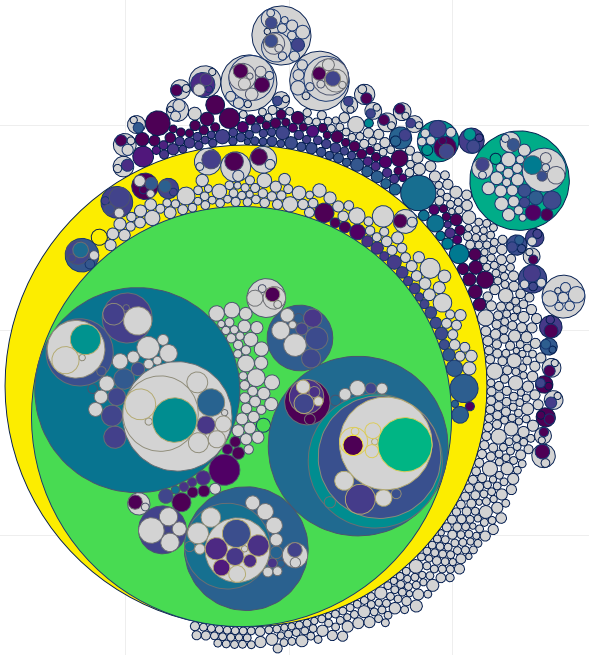
\includegraphics[width=0.9\linewidth]{img/kcc2tree} 

}

\caption{K-clique Community Structure.
\href{exh/kcc2tree.html}{\emph{Interactive pop-out.}}}\label{fig:kcc2tree}
\end{figure}

Figure \ref{fig:kcc2tree} shows a KCC model of the social sciences in
the first half of the twentieth century.

Disciplinarity and interdisciplinarity are revealed in a novel fashion
in the KCC model. Disciplinarity is shown as a level of exclusion.

\hypertarget{continents}{%
\subsection{Continents}\label{continents}}

The global map is made of many separate regions ranging in scale from
large continents to small isles. These regions are either shallowly
connected or entirely separated from each other. The vast majority of
these regions are ``flat isles'' with little to no internal structure of
their own. Most flat isles are supported by only a single article, some
by a couple of articles penned by the same author, and only a few
represent real activity among a small group of different authors.

\begin{figure}

{\centering 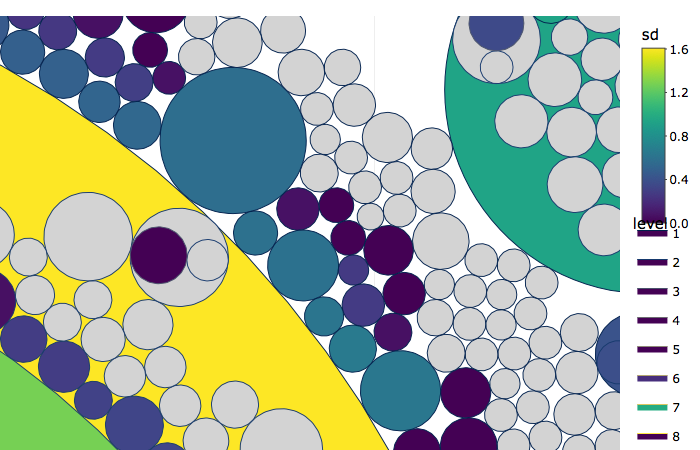
\includegraphics[width=0.9\linewidth]{img/flat-isle} 

}

\caption{Flat Isles, where Reviewers tend their Flock}\label{fig:flat-isle}
\end{figure}

The most substantial flat isle , the largest unenclosed and unenclosing
circle in Figure \ref{fig:flat-isle}, comes from four authors publishing
in the same 1930 \href{https://www.jstor.org/stable/i40084238}{issue} of
\emph{Zeitschrift Fur Nationalokonomie}. It includes 50 references the
most prominent of which are Angell's 1926 \emph{The Theory of
International Prices} and Tugwell's 1924 \emph{The Trends of Economics}.
The structure of the group is provided entirely by an article by Robert
Reisch ; the other three shared no references in common and Reisch's
article, titled ``The `Deposit'-Myth In Banking Theory'' and containing
108 references, is likely to have been written as an introduction to the
journal on the basis of what had already been accepted for publication.

Another flat isle of four articles has the exact same pattern, also from
\emph{Zeitschrift Fur Nationalokonomie} but from an
\href{https://www.jstor.org/stable/i40084262}{issue} in 1937, the
article on the first page of the issue, titled ``Theory Of Capital,
Introduction'' by von Hayek and containing 25 references, includes
subsections of the bibliographies of three other articles that do not
themselves overlap. Normally the longer a bibliography the more likely
it is that an article functions as a review linking other disparate
bibliographies. That von Hayek's article has such a short bibliography
and yet still links three otherwise separate articles confirms its
derivative character.

The following features then suggest when a flat isle represents an issue
introduction. All articles are published in the same issue. The removal
of the longest bibliography in the community yields a network of
disconnected components each uniquely representing the remaining bibs.
This longest bib is also either the first article in the issue or
precedes the others in pagination. These characteristics suggest
authorship internal to the editorial process itself. Later we will
explore how the removal of such articles helps to reveal ``bottom-up''
structure by removing the editorial advantage of certain authors to
bestow an ad hoc intellectual coherence on scholarship.

Table \ref{tab:iss-int} enumerates issue introductions and shows how
many are the structuring article in their community.

\begin{figure}

{\centering 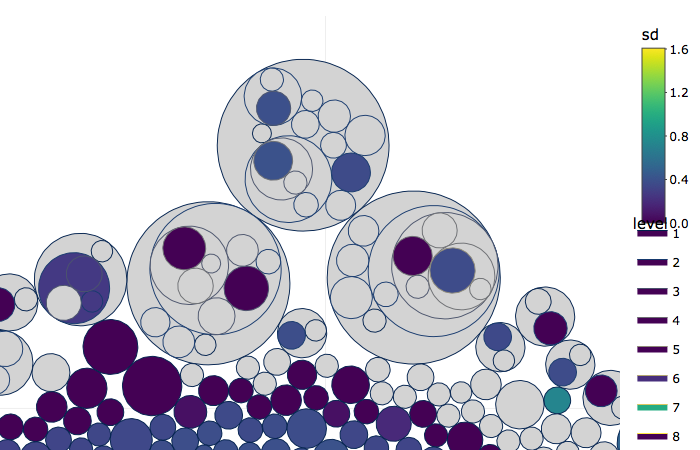
\includegraphics[width=0.9\linewidth]{img/hill-isle} 

}

\caption{Hill Isles, where the Wild Things Are}\label{fig:hill-isle}
\end{figure}

Reviews, whether they are self described as such, borrow directly from
the bibliographies of one or more seed articles, and in this way they
contribute a disproportionate amount of the global structure of the
co-reference network. This kind of review, rather than looking again at
an existing intellectual trend, creates the cohesion it purports to
describe. Flat isles, especially if they are large, are flat due to the
retrospection of a usually solitary reviewer. Compare this to ``hill
isles'' with more internal structure growing out of the related but
uncoordinated reference activity of authors.

\begin{figure}

{\centering \includegraphics[width=0.9\linewidth]{ambrose_dissertation_files/figure-latex/k3c1-22-1} 

}

\caption{Hill Isle in Graph Layout}\label{fig:k3c1-22}
\end{figure}

\hypertarget{peaks}{%
\subsection{Peaks}\label{peaks}}

The KCC model reveals

\hypertarget{valleys}{%
\subsection{Valleys}\label{valleys}}

\hypertarget{do-reference-lists-describe-author-knowledge}{%
\subsection{Do reference lists describe author
knowledge?}\label{do-reference-lists-describe-author-knowledge}}

The peer review process can now be thought of as a process of auditing
credentials. An author makes an opening bid with the submission of a
particular reference list. What this reference list implies about what
the author knows is unclear. One may omit a knowledge signal because it
is truthfully irrelevant or in a deceptive sin of omission oriented to
what they expect to be the expectations of editors and reviewers. One
may also include what they do not know out of error, braggadocio,
carelessness, or fraud. Part of the work of reviewers will be to
validate those claims to knowledge.




\begin{figure}

{\centering 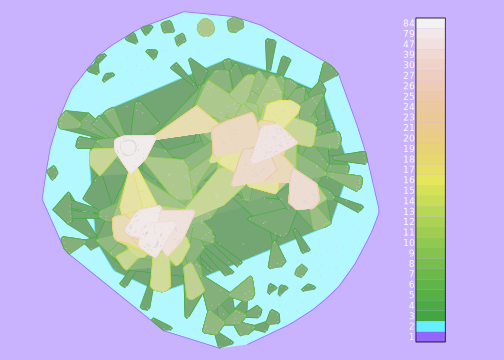
\includegraphics[width=0.9\linewidth]{ambrose_dissertation_files/figure-latex/kcc2isl-1} 

}

\caption{K-clique Community Island Plot.
\href{exh/isl3d.html}{\emph{Interactive pop-out.}}}\label{fig:kcc2isl}
\end{figure}

\bibliography{references.bib}


\end{document}
